\documentclass[12pt,a4paper,twoside,openright]{report}
\let\openright=\cleardoublepage



%%% Choose a language %%%

\newif\ifEN
\ENtrue   % uncomment this for english
%\ENfalse   % uncomment this for czech

%%% Configuration of the title page %%%

% \def\ThesisTitleStyle{mff} % MFF style
%\def\ThesisTitleStyle{cuni} % uncomment for old-style with cuni.cz logo
\def\ThesisTitleStyle{natur} % uncomment for nature faculty logo

% \def\UKFaculty{Faculty of Mathematics and Physics}
\def\UKFaculty{Faculty of Science}

\def\UKName{Charles University in Prague} % this is not used in the "mff" style

% Thesis type names, as used in several places in the title
% \def\ThesisTypeTitle{\ifEN BACHELOR THESIS \else BAKALÁŘSKÁ PRÁCE \fi}
\def\ThesisTypeTitle{\ifEN MASTER THESIS \else DIPLOMOVÁ PRÁCE \fi}
%\def\ThesisTypeTitle{\ifEN RIGOROUS THESIS \else RIGORÓZNÍ PRÁCE \fi}
%\def\ThesisTypeTitle{\ifEN DOCTORAL THESIS \else DISERTAČNÍ PRÁCE \fi}
% \def\ThesisGenitive{\ifEN bachelor \else bakalářské \fi}
\def\ThesisGenitive{\ifEN master \else diplomové \fi}
%\def\ThesisGenitive{\ifEN rigorous \else rigorózní \fi}
%\def\ThesisGenitive{\ifEN doctoral \else disertační \fi}
% \def\ThesisAccusative{\ifEN bachelor \else bakalářskou \fi}
\def\ThesisAccusative{\ifEN master \else diplomovou \fi}
%\def\ThesisAccusative{\ifEN rigorous \else rigorózní \fi}
%\def\ThesisAccusative{\ifEN doctoral \else disertační \fi}



%%% Fill in your details %%%

% (Note: \xxx is a "ToDo label" which makes the unfilled visible. Remove it.)
\def\ThesisTitle{Modeling spatio-temporal dynamics in primary visual cortex using deep neural network model}
\def\ThesisAuthor{Bc. David Beinhauer}
\def\YearSubmitted{2025}

% department assigned to the thesis
\def\Department{Department of Cell Biology}
% Is it a department (katedra), or an institute (ústav)?
\def\DeptType{Department}

\def\Supervisor{Mgr. Ján Antolík, Ph.D.}
\def\SupervisorsDepartment{Department of Cell Biology}

% Study programme and specialization
\def\StudyProgramme{Bioinformatics}
\def\StudyBranch{Bioinformatics}

\def\Dedication{%
I express my sincere gratitude to my supervisor, 
Mgr. Ján Antolík, Ph.D., for his unwavering guidance and support throughout
this project. Additionally, I am very grateful to Mgr. Luca Baroni for his valuable
insights and feedback. Finally, I extend my heartfelt gratitude
to my friends and family for their continuous support and encouragement throughout
my studies.
}

\def\AbstractEN{
    Recent advances in computational neuroscience and machine learning have enabled increasingly sophisticated models of neuronal systems. However, standard deep neural networks (DNNs) often prioritize task performance over biological plausibility, limiting their ability to capture complex neural dynamics.

    In this thesis, we propose a novel approach that integrates biologically inspired constraints into recurrent neural network (RNN) architectures to model the primary visual cortex (V1). Using synthetic data generated from a biologically detailed spiking neural network (SNN) model of cat V1, we develop RNN architectures incorporating anatomical structure alignment, excitatory-inhibitory neuron differentiation, biologically motivated neuronal modules, and synaptic depression mechanisms.

    Our results show that RNN architectures without complex internal modules can predict mean neuronal responses but struggle to capture full system dynamics. Introducing shared DNN neuron modules improves dynamics slightly, while RNN-based neuron modules substantially enhance the temporal fidelity of predictions. Conversely, synaptic depression modules did not improve performance, likely due to computational constraints and suboptimal hyperparameter tuning.

    This work demonstrates the promise of combining deep learning with biological realism to bridge the gap between predictive accuracy and interpretability, laying the groundwork for future applications to real neural recordings.
}

\def\AbstractCS{
    Nedávné pokroky v oboru výpočetních neurověd a strojového učení umožnily vývoj čím dál komplexnějších modelů neurálních systémů. Nicméně, standardní hluboké neurální sítě (DNN) často prioritizují celkovou úspěšnost v řešení zadaného problému nad biologickou interpretací, což limituje schopnost modelu zachytit komplexní neurální dynamiku.

    V rámci této práce navrhujeme nový způsob modelování kombinující biologické znalosti systému pro návrh modelů rekurentních neurálních sítí (RNN) primární zrakové kůry (V1). Za použití syntetických dat vygenerovaných z biologicky detailního impulzivního modelu neuronové sítě (SNN) kočičího V1, jsme vyvinuli RNN s anatomicky odpovídající architekturou rozlišující excitační a inhibiční neurony, používající biologicky motivované moduly neuronů a zapojující mechanismy synaptické deprese.

    Naše výsledky ukazují, že RNN síť bez použití komplexních modulů neuronů může predikovat průměrné neurální odpovědi, ale zaostává v zachycení komplexní dynamiky systému. Zapojení DNN modulů neuronů mírně zlepšuje dynamiku, nicméně výrazné zlepšení v predikci dynamiky systému přináší až zapojení RNN modulů neuronů. Naproti tomu moduly synaptické deprese nezlepšují dynamiku sítě, pravděpodobně kvůli výpočetním omezením a neoptimální volbě hyperparametrů.

    Tato práce vykazuje potenciál kombinace hlubokých neurálních sítí s biologickými znalostmi umožňující kombinaci přesnosti predikcí s interpretovatelností a vytváří základy pro budoucí aplikace na reálných experimentálních datech.
}

% 3 to 5 keywords (recommended), each enclosed in curly braces.
% Keywords are useful for indexing and searching for the theses by topic.
\def\Keywords{%
{visual cortex}, {recurrent networks}, {model deep neural networks}
}

% If your abstracts are long and do not fit in the infopage, you can make the
% fonts a bit smaller by this setting. (Also, you should try to compress your abstract more.)
% Alternatively, consider increasing the size of the page by uncommenting the
% geometry modification in thesis.tex.
\def\InfoPageFont{}
%\def\InfoPageFont{\small}  %uncomment to decrease font size

\ifEN\relax\else
% If you are writing a czech thesis, you additionally need to fill in the
% english translation of the metadata here!
\def\ThesisTitleEN{\xxx{Thesis title in English}}
\def\DepartmentEN{\xxx{Name of the department in English}}
\def\DeptTypeEN{\xxx{Department}}
\def\SupervisorsDepartmentEN{\xxx{Superdepartment}}
\def\StudyProgrammeEN{\xxx{study programme}}
\def\StudyBranchEN{\xxx{study branch}}
\def\KeywordsEN{%
\xxx{{key} {words}}
}
\fi


\usepackage[a-2u]{pdfx}

\ifEN\else\usepackage[czech,shorthands=off]{babel}\fi

% See https://en.wikipedia.org/wiki/Canons_of_page_construction before
% modifying the size of printable area. LaTeX defaults are great.
% If you feel it would help anything, you can enlarge the printable area a bit:
%\usepackage[textwidth=390pt,textheight=630pt]{geometry}
% The official recommendation expands the area quite a bit (looks pretty harsh):
%\usepackage[textwidth=145mm,textheight=247mm]{geometry}

%%% TYPICAL FONT CHOICES (uncomment what you like) %%%
% Recommended combo: Libertinus (autoselects Biolinum for sans) and everything
% else (math+tt) comes from Latin Modern)
\usepackage{lmodern}
\usepackage[mono=false]{libertinus}

% For the "classic" LaTeX fonts (very good for pure math theses), simply
% comment out the libertinus package above.

% IBM Plex font suite: nice, but requires us to fine-tune the sizes and does
% not directly support small caps (\textsc):
%\usepackage[usefilenames,RM={Scale=0.88},SS={Scale=0.88},SScon={Scale=0.88},TT={Scale=0.88},DefaultFeatures={Ligatures=Common}]{plex-otf}

% TeX Gyre combo (Pagella+Heros+Cursor)
%\usepackage{fontspec}
%\setmainfont{TeX Gyre Pagella}
%\setsansfont{TeX Gyre Heros}
%\setmonofont{TeX Gyre Cursor}

% some useful packages
\usepackage{microtype}
\usepackage{amsmath,amsfonts,amsthm,bm}
\usepackage{graphicx}
\usepackage{xcolor}
\usepackage{booktabs}
\usepackage{caption}
\usepackage{floatrow}
\usepackage{derivative}

% Bibliography formatting.
% CHECK THE REQUIREMENTS OF YOUR DEPARTMENT AND FACULTY ON THE CITATION FORMAT!
%
% These are relatively "safe" default options that most people use:
\usepackage[natbib,style=numeric,sorting=none]{biblatex}
% alternative with alphanumeric citations (more informative than numbers, and
% more common in computer science journals):
% \usepackage[natbib,style=alphabetic]{biblatex}
%
% ALTERNATIVES THAT CONFORM TO ISO690
% ISO690 is not the greatest citation format ever, but may be formally
% required at Charles University, depending on your faculty and department.
%\usepackage[natbib,style=iso-numeric,sorting=none]{biblatex}
%\usepackage[natbib,style=iso-alphabetic]{biblatex}
% You might want to add extra options such as `maxbibnames=6,maxcitenames=2`
% here to further conform to some of the formatting requirements (see below for
% details). Again, consult your faculty rules.
%
% Additional option choices:
%  - add `giveninits=true` to typeset "E. A. Poe" instead of full Edgar Allan
%  - `terseinits=true` additionaly shortens it to nature-like "Poe EA"
%  - add `maxnames=10` to limit (or loosen) the maximum number of authors in
%    bibliography entry before shortening to `et al.` (useful when referring to
%    book collections that may have hundreds of authors)
%  - use `maxcitenames=2` to finetune the amount of authors listed in text-cite
%    commands (\citet). Corresponding option that only affects the bibliography
%    is `maxbibnames=10`.
%  - `sorting=none` causes the bibliography list to be ordered by the order of
%    citation as they appear in the text, which is usually the desired behavior
%    with numeric citations. Additionally you can use a style like
%    `numeric-comp` that compresses the long lists of citations such as
%    [1,2,3,4,5,6,7,8] to simpler [1--8]. This is especially useful if you plan
%    to add tremendous amounts of citations, as usual in life sciences and
%    bioinformatics.
%  - if you don't like the "In:" appearing in the bibliography, use the
%    extended style (`ext-numeric` or `ext-alphabetic`), and add option
%    `articlein=false`.
%
% possibly reverse the names of the authors with the default styles:
%\DeclareNameAlias{default}{family-given}

% load the file with bibliography entries
\addbibresource{refs.bib}

% remove this if you won't use fancy verbatim environments
\usepackage{fancyvrb}

% remove this if you won't typeset TikZ graphics
\usepackage{tikz}
\usetikzlibrary{positioning} %add libraries as needed (shapes, decorations, ...)

% remove this if you won't typeset any pseudocode
\usepackage{algpseudocode}
\usepackage{algorithm}

% remove this if you won't list any source code
\usepackage{listings}


\hypersetup{unicode}
\hypersetup{breaklinks=true}

\usepackage[noabbrev]{cleveref}


% various forms of TODOs (you should remove this before submitting)
\usepackage[textsize=tiny, backgroundcolor=yellow!25, linecolor=black!25]{todonotes}
\newcommand{\xxx}[1]{\textcolor{red!}{#1}}

 % remove this before compiling the final version


% use this for typesetting a chapter without a number, e.g. intro and outro
\def\chapwithtoc#1{\chapter*{#1}\addcontentsline{toc}{chapter}{#1}}

% If there is a line/figure overflowing into page margin, this will make the
% problem evident by drawing a thick black line at the overflowing spot. You
% should not disable this.
\overfullrule=3mm

% The maximum stretching of a space. Increasing this makes the text a bit more
% sloppy, but may prevent the overflows by moving words to next line.
\emergencystretch=1em

\ifEN
\theoremstyle{plain}
\newtheorem{thm}{Theorem}
\newtheorem{lemma}[thm]{Lemma}
\newtheorem{claim}[thm]{Claim}
\newtheorem{defn}{Definition}
\theoremstyle{remark}
\newtheorem*{cor}{Corollary}
\else
\theoremstyle{plain}
\newtheorem{thm}{Věta}
\newtheorem{lemma}{Lemma}
\newtheorem{claim}{Tvrzení}
\newtheorem{defn}{Definice}
\theoremstyle{remark}
\newtheorem*{cor}{Důsledek}
\fi

\newenvironment{myproof}{
  \par\medskip\noindent
  \textit{\ifEN Proof \else Důkaz \fi}.
}{
\newline
\rightline{$\qedsymbol$}
}

% real/natural numbers
\newcommand{\R}{\mathbb{R}}
\newcommand{\N}{\mathbb{N}}

% Number only selected equations in align
\newcommand{\numberthis}{\addtocounter{equation}{1}\tag{\theequation}}

% asymptotic complexity
\newcommand{\asy}[1]{\mathcal{O}(#1)}

% listings and default lstlisting config (remove if unused)
\DeclareNewFloatType{listing}{}
\floatsetup[listing]{style=ruled}

\DeclareCaptionStyle{thesis}{style=base,font={small,sf},labelfont=bf,labelsep=quad}
\captionsetup{style=thesis}
\captionsetup[algorithm]{style=thesis,singlelinecheck=off}
\captionsetup[listing]{style=thesis,singlelinecheck=off}

% Customization of algorithmic environment (comment style)
\renewcommand{\algorithmiccomment}[1]{\textcolor{black!25}{\dotfill\sffamily\itshape#1}}

% Uncomment for table captions on top. This is sometimes recommended by the
% style guide, and even required for some publication types.
%\floatsetup[table]{capposition=top}
%
% (Opinionated rant:) Captions on top are not "compatible" with the general
% guideline that the tables should be formatted to be quickly visually
% comprehensible and *beautiful* in general (like figures), and that the table
% "head" row (with column names) should alone communicate most of the content
% and interpretation of the table. If you just need to show a long boring list
% of numbers (because you have to), either put some effort into showing the
% data in an attractive figure-table, or move the data to an attachment and
% refer to it, so that the boredom does not impact the main text flow.
%
% You can make the top-captions look much less ugly by aligning the widths of
% the caption and the table, with setting `framefit=yes`, as shown below.  This
% additionally requires some extra markup in your {table} environments; see the
% comments in the example table in `ch2.tex` for details.
%\floatsetup[table]{capposition=top,framefit=yes}

\ifEN\floatname{listing}{Listing}
\else\floatname{listing}{Výpis kódu}\fi
\lstset{ % use this to define styling for any other language
  language=C++,
  tabsize=2,
  showstringspaces=false,
  basicstyle=\footnotesize\tt\color{black!75},
  identifierstyle=\bfseries\color{black},
  commentstyle=\color{green!50!black},
  stringstyle=\color{red!50!black},
  keywordstyle=\color{blue!75!black}}

% Czech versions of the used cleveref references (It's not as convenient as in
% English because of declension, cleveref is limited to sg/pl nominative. Use
% plain \ref to dodge that.)
\ifEN\relax\else
\crefname{chapter}{kapitola}{kapitoly}
\Crefname{chapter}{Kapitola}{Kapitoly}
\crefname{section}{sekce}{sekce}
\Crefname{section}{Sekce}{Sekce}
\crefname{subsection}{sekce}{sekce}
\Crefname{subsection}{Sekce}{Sekce}
\crefname{subsubsection}{sekce}{sekce}
\Crefname{subsubsection}{Sekce}{Sekce}
\crefname{figure}{obrázek}{obrázky}
\Crefname{figure}{Obrázek}{Obrázky}
\crefname{table}{tabulka}{tabulky}
\Crefname{table}{Tabulka}{Tabulky}
\crefname{listing}{výpis}{výpisy}
\Crefname{listing}{Výpis}{Výpisy}
\floatname{algorithm}{Algoritmus}
\crefname{algorithm}{algoritmus}{algoritmy}
\Crefname{algorithm}{Algoritmus}{Algoritmy}
\newcommand{\crefpairconjunction}{ a~}
\newcommand{\crefrangeconjunction}{ a~}
\fi
 % use this file for various custom definitions


\begin{document}

% the layout is mandatory, edit only in dire circumstances

\pagestyle{empty}
\hypersetup{pageanchor=false}
\begin{center}

% top part of the layout, this actually differs between faculties

\def\ThesisTitleXmff{%
  \ifEN
    \centerline{\mbox{
\includegraphics[width=166mm]{img/logo-en.pdf}}}
  \else
    \centerline{\mbox{
\includegraphics[width=166mm]{img/logo-cs.pdf}}}
  \fi
  \vspace{-8mm}\vfill%
  {\bf\Large\ThesisTypeTitle}
  \vfill%
  {\LARGE\ThesisAuthor}\par
  \vspace{15mm}%
  {\LARGE\bfseries\ThesisTitle}
  \vfill%
  \Department}
\def\ThesisTitleCuniLogo#1{%
  {\large\UKName\par\medskip\par\UKFaculty }
  \vfill%
  {\bf\Large\ThesisTypeTitle}
  \vfill%
  \includegraphics[width=70mm]{#1}
  \vfill%
  {\LARGE\ThesisAuthor}\par
  \vspace{15mm}%
  {\LARGE\bfseries\ThesisTitle}
  \vfill%
  \Department\par}
\def\ThesisTitleXcuni{\ThesisTitleCuniLogo{img/uklogo.pdf}}
\def\ThesisTitleXnatur{\ThesisTitleCuniLogo{img/naturlogo.pdf}}

% choose the correct page and print it
\csname ThesisTitleX\ThesisTitleStyle\endcsname
% latex corner: X is the new @

\vfill

{
\centerline{\vbox{\halign{\hbox to 0.45\hsize{\hfil #}&\hskip 0.5em\parbox[t]{0.45\hsize}{\raggedright #}\cr
\ifEN Supervisor of the \ThesisGenitive thesis:
\else Vedoucí \ThesisGenitive práce: \fi
& \Supervisor \cr
\noalign{\vspace{2mm}}
\ifEN Study programme: \else Studijní program: \fi
& \StudyProgramme \cr
\noalign{\vspace{2mm}}
\ifEN Study branch: \else Studijní obor: \fi
& \StudyBranch \cr
}}}}

\vfill

\ifEN Prague \else Praha \fi
\YearSubmitted

\end{center}

\newpage

% remember to sign this!
\openright
\hypersetup{pageanchor=true}
\pagestyle{plain}
\pagenumbering{roman}
\vglue 0pt plus 1fill

\ifEN
\noindent
I declare that I carried out this \ThesisAccusative thesis on my own, and only with the cited sources, literature and other professional sources. I understand that my work relates to the rights and obligations under the Act No. 121/2000 Sb., the Copyright Act, as amended, in particular the fact that the Charles University has the right to conclude a license agreement on the use of this work as a school work pursuant to Section 60 subsection 1 of the Copyright Act.
\else
\noindent
Prohlašuji, že jsem tuto \ThesisAccusative práci vypracoval(a) samostatně a~výhradně s~použitím citovaných pramenů, literatury a~dalších odborných zdrojů. Beru na vědomí, že se na moji práci vztahují práva a~povinnosti vyplývající ze zákona č.~121/2000 Sb., autorského zákona v platném znění, zejména skutečnost, že Univerzita Karlova má právo na uzavření licenční smlouvy o~užití této práce jako školního díla podle § 60 odst. 1 autorského zákona.
\fi

\vspace{10mm}


\ifEN
\hbox{\hbox to 0.5\hsize{%
In \hbox to 6em{\dotfill} date \hbox to 6em{\dotfill}
\hss}\hbox to 0.5\hsize{\dotfill\quad}}
\smallskip
\hbox{\hbox to 0.5\hsize{}\hbox to 0.5\hsize{\hfil Author's signature\hfil}}
\else
\hbox{\hbox to 0.5\hsize{%
V \hbox to 6em{\dotfill} dne \hbox to 6em{\dotfill}
\hss}\hbox to 0.5\hsize{\dotfill\quad}}
\smallskip
\hbox{\hbox to 0.5\hsize{}\hbox to 0.5\hsize{\hfil Podpis autora\hfil}}
\fi

\vspace{20mm}
\newpage

% dedication

\openright

\noindent
\Dedication

\newpage

% mandatory information page

\openright

\vbox to 0.49\vsize{\InfoPageFont
\setlength\parindent{0mm}
\setlength\parskip{5mm}

\ifEN Title: \else Název práce: \fi
\ThesisTitle

\ifEN Author: \else Autor: \fi
\ThesisAuthor

\DeptType:
\Department

\ifEN Supervisor: \else Vedoucí \ThesisGenitive práce: \fi
\Supervisor, \SupervisorsDepartment

\ifEN Abstract: \AbstractEN \else Abstrakt: \AbstractCS \fi

\ifEN Keywords: \else Klíčová slova: \fi
\Keywords

\vss}\ifEN\relax\else\nobreak\vbox to 0.49\vsize{\InfoPageFont
\setlength\parindent{0mm}
\setlength\parskip{5mm}

Title:
\ThesisTitleEN

Author:
\ThesisAuthor

\DeptTypeEN:
\DepartmentEN

Supervisor:
\Supervisor, \SupervisorsDepartmentEN

Abstract:
\AbstractEN

Keywords:
\KeywordsEN

\vss}
\fi

\newpage

\openright
\pagestyle{plain}
\pagenumbering{arabic}
\setcounter{page}{1}


\tableofcontents


\chapwithtoc{Introduction}

Significant advancements in neurobiology have been made over 
the past few decades. The development of new technologies and 
methods has provided researchers with a diverse set of tools to
study the brain. With the rise of highly parallelized computing, 
computational neuroscience has become one of the most important 
approaches to studying neuronal systems (\citet{trappenberg2009fundamentals}), 
offering new perspective on
brain function. It has enabled the simulation of large-scale neuronal 
networks, allowing us to analyze their behavior without relying solely
on vast amounts of real-world experimental data. As a result, we can 
now investigate brain systems in greater detail and gain a more precise 
understanding of their underlying principles.

With the rapid expansion of the machine learning, particularly deep neural 
network (DNN) models, neuroscientists have sought to apply these techniques
too. State-of-the-art convolutional DNN models have demonstrated outstanding
performance in task such as image classification and object detection 
(\citet{krizhevsky2012imagenet}, \citet{li2014medical}). 
These methods have also been used to model certain brain regions, often
yielding promising results. However, they come
with significant limitations (\citet{celeghin2023convolutional}).
Traditionally researchers using DNNs typically disregard the anatomical structure
and constraints of real neuronal networks. For instance, they rely exclusively on 
feed-forward architecture, whereas real brain networks are highly recurrent.
The models then typically prioritize task performance over biological plausibility
and interpretability.

On the other hand, usage of biologically plausible models such as 
spiking neural network (SNN) models have been a fundamental approach in computational
neuroscience (\citet{ghosh2009spiking}, \citet{yamazaki2022spiking}). 
These models attempt to bridge biological knowledge with computational
methods by incorporating biologically relevant constraints, preventing overfitting to
training datasets. However, SNNs face their own challenges, particularly the need 
to precise mathematical formulations to define networks behaviors, which can
limit their flexibility and scalability (\citet{izhikevich2004model}).

One of the most widely studied yet complex brain regions is the visual cortex.
Due to its intricate structure, studying it directly is almost impossible.
It makes the computational approaches essential for understanding it. 
Thanks to extensive experimental research the subregion called primary visual 
cortex (V1) is the best understood (\citet{miikkulainen2006computational}). 
Modern research on V1 typically employs 
either CNNs or SNNs, but both approaches have notable 
drawbacks (\citet{niell2021cortical}).

In this work, we aim to overcome the limitations of DNN models by 
integrating biological constraints into their design to better 
understand primary visual cortex (V1). We train our model
to predict the neuronal responses based on SNN model of cat's V1,
developed by \citet{antolik2024comprehensive}. Specifically, we
focus on predicting neuronal responses in layer IV (L4)
and layer II/III (L2/3) of V1 using input from the 
lateral geniculate nucleus (LGN) neurons. 

Although we train our model on synthetic data from the SNN, 
our goal is to achieve strong predictive performance on real V1 
neuronal recordings as well.To accomplish this, we utilize biologically
constrained recurrent DNN model to study a selected region of V1, 
incorporating the following constraints.

\begin{description}
    \item[Anatomical structure alignment:] The architecture of our
    model is layered according to known anatomical constraints. Each
    neuron in the network corresponds to a specific neuron in the real
    system. It significantly facilitates teh interpretability of model
    parameters. This biologically grounded approach enables us to study
    the dynamics of the visual cortex in a more realistic manner and 
    gain insights that align with actual neural processes.

    \item[Excitatory and inhibitory neuron differentiation:] We explicitly
    distinguish between excitatory and inhibitory neurons, enforcing 
    biologically plausible behavior within the architecture and ensuring 
    that specific neuronal types function as expected.
    
    \item[Biologically inspired activation functions:] Instead of standard
    activation functions such as ReLU or tanh, we introduce small shared
    DNN modules across anatomically defined layers. These modules aim to
    approximate the complexity of real neuronal transfer functions. They
    pursue capturing nonlinearities and allowing neurons to retain a form
    of memory that adapts to previous stimuli.

    \item[Synaptic adaptation modules:] To model the plasticity of neuronal
    synapses, we incorporate modules that adjust synaptic responses based on
    increased stimuli rates from specific neuronal layers. This mechanism aims
    to reflect real-life synaptic adaptation processes observed in biological 
    networks.
\end{description}

By embedding these anatomical constraints into our model, we aim to
enhance both the predictive power and interpretability of neural simulations,
ultimately contributing to a better understanding of the selected brain region.

In our research we have obtained the following results. 
\begin{description}
    \item Usage of the recurrent DNN model with biologically constraint 
    architecture without the DNN modules of the neurons captures the 
    mean neuronal responses reasonably well. Although, there is still
    room for improvement in terms of capturing the model dynamics.
    \item Usage of shared DNN modules of neurons significantly improved the
    model performance especially in terms of model dynamics.
    \item Differentiation in inputs from excitatory and inhibitory
    neurons to neuronal DNN module slightly improves the predictions in
    comparison to propagating the input signal without differentiation
    of the neuronal types.
    \item Usage of RNN model with LSTM cells of shared neuronal module
    slightly improved the performance of the model. This we address to
    introduction of neuron memory to the model.
    \item Usage of synaptic adaptation module does not improve the
    spatio-temporal resolution of the model in spite of introduction of 
    the synaptic memory. This might well be because of non-suitability of
    the tested hyperparameters.
\end{description}

The thesis is structured into several sections. In the first section
we introduce the reader to the theoretical background of the computational
neuroscience with the main focus on the visual processing and especially
to primary visual cortex (V1). Alongside with this, we introduce the reader
with the classical model that is spiking models and to selected intrinsical
aspects from the machine learning field. In the second section, we profoundly
describe our approach in the modeling of the system. We describe the architecture
of our model, dataset and evaluation metrics there. In the third section
we provide the experimental results of our study.



\chapter{Early Visual System}
\label{chap:visual_system}
In our thesis we are focussing in modeling the primary visual cortex (V1)
which plays a significant role in the early visual processing in the
mammalian brain. This area is widely studied and has been a subject of
research for many decades. In this chapter we will focus mainly on the 
parts closely related to our work. Thus, the comprehensive description
of the system can be seen for example in the "Bear book". 

\section{General Structure of the Early Visual System}
\label{sec:general_structure}
Overall, the areas responsible for the visual processing covers nearly 
a half of the human brain. The first stage of the visual processing happens in
the so called Early Visual System.

The visual signal travels in form of light through the complex light modulating
system of the eye and is projected onto the retina. The retina is a thin layer
of neural tissue that is responsible for light detection and initial processing.
The signal then travels through the optic nerve to the optic chiasm, where the 
signals are split based on the visual field side, and then travel through the
optic tract to the lateral geniculate nucleus (LGN) of the thalamus. The LGN is
responsible fort the initial processing of the visual signal and then sends majority
of the signal to the primary visual cortex (V1) through the optic radiation. The
V1 is the first cortical area that is fully specialized for visual processing. 
First more complex computations are done there. When the signal leaves the V1,
it is further processed int the higher visual areas that are responsible for the
high level visual processing.

\section{Eye}
\label{sec:eye}
One of the key objectives of an eye is to collect the electromagnetic signal
from the environment bundle it using the complex optical system and project it
onto the retina. The eye comprises of several specialized parts that appropriately
modulates and bends the light. For the comprehensive descriptions of these 
parts see image (TODO: image with eye description) or the appropriate literature
(TODO: citation to comprehensive eye description).

\subsection{Retina}
\label{subsec:retina}
Second important function of the eye is to convert and preprocess the 
light signal into the neural signal that can be further processed in the brain.
This is done by the retina. It is thin layer of neural tissue located at the back
of eye. It is composed of several types of cells and layers each of them responsible
for different part of signal modulation. These cells are visual receptors,
bipolar cells, horizontal cells, amacrine cells and ganglion cells.

The first cells in the manaegerie of visual processing are the \emph{photoreceptor cells}
called \emph{rods} and \emph{cones}. These cells exploits the photochemical reaction of the 
proteins located in their outer segments to convert the light signal into the
chemical signal. The rods are very sensitive to small light intensities, 
detect wide range of wavelengths and are responsible for the low light vision.
On the other hand cone are selective only for the specific wavelengths and their
sensitivity to lower light intensities is much lower. They are responsible for the
color and acuity vision. The distribution of these cells is not uniform across
the retina. The fovea, the central part of the retina, is rich in cones. On the other
hand the periphery of the retina is mainly populated by the rods. It is worth
mentioning that there there is also a small region called the blind spot where
the optic nerve leaves the eye and there are thus no photoreceptors. The 
visual description of the photoreceptor distribution and retina structure we
provide the image (TODO: image of the retina, photoreceptor distribution). Finally,
it is worth noting tha that when the photoreceptors are activated, they hyperpolarized
which results in releasing the neurotransmitter glutamate. This neurotransmitter
is then detected by the bipolar cells. This feature in some modifications is 
typical for all the retina cells except the ganglion cells that elicits the 
action potential typical for the neural cells.

The signal from the photoreceptors is then further processed by the 
\emph{bipolar cells}. Their amount is around 10M and they summarize the 
information from around 125 millions of photoreceptors. The amount of the 
photoreceptors they connect is dependent on the location and type of the 
photoreceptor it connects. These cells closely cooperate with the 
\emph{horizontal cells} that overarches wider range of the photoreceptors
and provides the signal about surrounding light intensity to bipolar cells.

The bipolar cells are divided into two types: \emph{ON bipolar cells} and 
\emph{OFF bipolar cells}. The difference between these two types is in the 
way they react to the light signal. The ON bipolar cells are activated when there
is a light signal present, while the OFF bipolar cells are activated when there is not
the signal. They react positively to the light signal from the center of the receptory
field and negatively to the light signal from the surrounding area that is gathered by the
horizontal cells. The receptive field is basically circumscribed area of the photoreceptors. The 
radius changes based on the type and position of in the retina.

The signal then travels to the \emph{ganglion cells} that closely cooperate with the 
amacrine cells. The way principle of the signal processing in this layer is analogical to 
the processing in the bipolar cells and the horizontal cells. The ganglion cells are the 
first cells that elicit the action potential. It is due to the fact that they connect the
retina with the brain and the signal thus need to travel longer distance. The axons of these
cells then terminates in the \emph{Lateral Geniculate Nucleus (LGN)} of the thalamus.

\section{Lateral Geniculate Nucleus}
\label{sec:lgn}
The following steps in the visual processing happen in the 
\emph{Lateral Geniculate Nucleus (LGN)}. It is a part of the thalamus on each side of the 
brain responsible for the initial processing of the visual signal. It is the region where
the majority of the optic tract fibers terminate. Majority of the outputs from this region
then travel to the \emph{primary visual cortex (V1)} through the optic radiation. Where is
the center of the conscious visual perception. The defects in the pathway from the retina 
to the LGN and to the V1 can lead to blindness. Thanks to the structure of the visual
pathway we can tract the defects in the visual system to the specific location. It 
is worth mentioning that majority of the input to the LGN comes from the V1. Currently, 
it is not clear the exact role of these connections but it is believed that they are mainly
responsible for the feedback and modulation of the signal.

The LGN is composed of six layers. These are split into half for each eye. The receptive
fields of the similar to retinal cells concentric.

\section{Primary Visual Cortex}
\label{sec:v1}
The primary visual cortex (V1) is the first cortical area that is fully specialized for 
the visual processing. It is located in the occipital (back) lobe of the brain. The 
V1 is responsible for the initial processing of the visual stimuli. It encodes for example
the orientation, size, motion and color. The output is then split into the two streams
the P-Stream responsible for orientation and location and the M-stream responsible for 
the motion.

The V1 is composed of six layers (typically named by Roman numerals). The input from 
the LGN is mainly sent to the layer IV. This layer is further subdivided into four 
sublayers (A, B, C$\alpha$ and C$\beta$). It is responsible for the initial processing
and is mainly specialized for monoocular input. The output is then sent mostly to the the 
layers II and III. These layers are functionally very similar and are typically labeled
as one layer II/III. Since this part the binocular processing prevails. The output is
then sent to the extrastriate areas like V2, V3 etc. that are responsible for the higher 
level visual processing. The rest of the layers I, V and VI are responsible mainly for 
the feedback and modulation of the signal. 

It is worth mentioning that mainly in layer IV there is a high range of interlayer connections.
Alongside with this in each layers there are also the inhibitory neurons that are 
also connected only in intra-layer manner and only affect the neurons in the same layer.
On the contrary some excitatory neurons does spread across the layers.

In the V1 there is still an important phenomenon present called the \emph{retinoscopy}.
It is the phenomenon where the neurons in the V1 are organized in the way that 
corresponds to the retinal organization. This means that the neurons closer to each
other in V1 correspond to neurons that are also close to each other in LGN and retina.
It is worth mentioning that the mapping is not uniformly precise since some parts of 
the visual field are densely covered than others (center and periphery of the visual field).

\subsection{Receptive field properties of V1 cells}
\label{subsec:receptive_field}
The neurons in V1 are specialized in several types responsible for the different properties
of the visual stimuli. These types creates overlapping interconnected maps that cover 
all of these properties. The properties are the following:

\begin{description}
    \item[Orientation selectivity:] Since layers IVC ($\alpha$ and $\beta$) the  
    orientation field stops to be circular and becomes elongated. The neurons in the 
    layer IVC are thus selective for the orientation of the visual stimuli. In other
    words they prefer the signal of the line in specific angle. In fact this preferred
    periodically changes across the V1 which results in similar orientation preferences
    in the close vicinity of the neurons. In terms of orientation selectivity 
    we also distinguish between \emph{simple} and \emph{complex} cells.
    \begin{description}
        \item[Simple cells:] These cells are selective for the orientation of the line 
        and the position of the line. In other words they are similar to ON and OFF cells
        from the previous layers. Its input is basically the sum several ON and OFF cells 
        from the LGN. 
        \item[Complex cells:] These cells are selective for the orientation of the line
        but anywhere in the orientation field. In other words they do not have any 
        ON and OFF regions. Its input is the sum of the simple cells.
    \end{description} 

    \item[Direction selectivity:] Some of the V1 neurons are specialized for the detection
    of motion in perpendicular direction.
    \item[Binocularity:] Till the layer IV the neurons are mainly monocular. This
    changes in the future layers. The neurons then combine the information from both eyes 
    and need to properly overlap the same information.
    \item[Other types:] The rest of the neurons are specialized for instance for motion, 
    depth, feedback or color.
\end{description}

\section{Extrastriate Visual Cortex}
\label{sec:extrastriate}
After the signal leaves the V1 it is further processed in the higher visual areas.
These areas are responsible for more complex visual processing and deficits in these 
typically result in some perceptual deficits but not the overall blindness.


\chapter{Computational Neuroscience}
\label{chap:computation_neuroscience}
Computational neuroscience is an interdisciplinary field that
utilizes mathematics and computer science knowledge to better
understand the nervous system and brain. With the rampant
ascent of the computational efficiency and technology for
obtaining more data from the experiments this field
became more and more relevant. Especially, in the last
years with the ascent of the DNNs. The models are great due for
its replicability, stability. It does not contain any noise and so on.

In computational neuroscience we commonly define three categories of models
\citet{dayan2005theoretical}. These models are \emph{descriptive} that summarize
large number of experimental data and describe what the system does. There models
might also be biologically plausible but its main goal is to describe the 
system, not to explain it. The example of it might be some mathematical description
of the behavior of the specific aspect of the brain like receptive field of a neuron 
or spiking rate of the neuron.
The second type is \emph{mechanistic} model, these 
models aim to explain how the system works on the anatomical level. The last
type is \emph{interpretive} model, these models use information and computational
principles to explore the cognitive and behavioral functions of the system, and they 
try to address why the system operates as it does. Overall,
it is typically not clear which model suits the problem the best and often the models
itself overlap the categories. This thesis might be a great example of the overlap of
the categories, where we try to accurately
describe the behavior, alongside with this we try to explain the behavior as we 
focus on the model explainability. As a result, we can say our model kind of overlaps
all of the categories.

In the following sections, we will describe the most common terms in the computational
neuroscience fields, typical evaluation approaches and we will list the selected 
modeling approaches that are used in the field.

\section{Introduction to System Identification in Visual System}
\label{sec:system_identification}
Since our thesis is focused on the study of the visual system we will focus mainly on
introducing the aspects closely related to the study of visual system. It is
worth noting though that the primary visual cortex and visual system overall is one of
the most studied ones in the computational neuroscience and thus a wide range of the
terms has been introduced and defined on the example of the visual system (TODO: cite
Abott paper). 

Characterizing the relationship between stimulus and neuronal response is a complex
task since it does not only depend on the stimulus itself but also on the other 
factors such as temporal state of the neuron, temporal separation between the stimuli
and many others. Because of that the neuronal responses might differ in trials on 
the same stimuli.This makes accurate prediction of the single neuronal spike almost 
impossible. Instead, we try to capture the probability distribution and perform well 
across all the trials. Typically, many neurons respond to a given stimuli, so, 
the properties of the stimulus are encoded in the large population of neurons and thus 
it is arguable more important to understand and properly describe the whole 
population of neurons rather than just perform well on the single neuron predictions.

The nice overview of the system identification can be seen in 
\citet{annurev:/content/journals/10.1146/annurev-vision-091718-014731} which served as
a source of information for the following sections.

\subsection{System Identification}
\label{subsec:system_identification}
The task of the system identification is to estimate and describe the unknown system 
based on the measured data 
\citet{annurev:/content/journals/10.1146/annurev-vision-091718-014731}. 
In the context of the visual system, the system is the
corresponding neuronal population and the measured data consists typically of the visual 
stimuli and the corresponding neuronal responses. In the typical approach we 
separate the data to input data and output data. Overall we can define the task of 
system identification as the following:

\begin{equation}
    r = f(s)
    \label{eq:system_identification}
\end{equation}

Where $s$ is the stimulus, $r$ is the response of the system typically in form of 
spikes or spike trains on the stimulus and 
$f$ is the unknown mapping function that describes the system. Our goal is to 
estimate the function $f$.

\subsection{Stimulus}
\label{subsec:stimulus}
The stimulus can be any input signal that can invoke the response. Typically it is 
represented as a vector or a matrix or a sequence of them of the appropriate values. 
In the context of the visual system, the stimulus is typically the image or the 
sequence of images (or video) that are typically represented as a matrix.

The general problem with the stimuli is what kind of the stimuli is appropriate 
for the given task \citet{carandini2005we}. The typically used stimuli were the 
simple arbitrary stimuli like bars or sinusoidal grating patterns for example in 
\citet{hubel1965receptive}'s work. However, these
stimuli are not very informative as they do not really occur in the real world.

Another widely used method is the white-noise stimuli \citet{dayan2005theoretical},
\citet{chichilnisky2001simple}. The idea under this stimuli is 
that each pixel of the image stimulus should be independent to each other. This 
if defined correctly should cover uniformly the whole space of the possible visual 
stimuli. Although it has been proven that this stimuli is to some extend very 
informative there are also several drawbacks related to it \citet{Talebi1560}. 
Mainly the thing that since neurons evolved to primary process the natural stimuli, 
the white-noise stimuli does not affect especially neurons highly specialized to 
some aspect of the natural stimuli enough. 

This is the reason why many of the recent 
researches focus on the natural stimuli \citet{sonkusare2019naturalistic}, 
\citet{lurz2020generalization}, \citet{antolik2024comprehensive}. Using this we can 
encounter alongside with other properties of the neuronal receptive fields also the 
selectivity of the neurons to typical properties of the natural stimuli.

\subsection{Spike Trains}
\label{subsec:spike_trains}
Neurons propagate information through action potentials often called \emph{spikes}. 
Although, it is typical that they differ in variety of properties like duration, 
amplitude and shape, we typically 
treat them as binary identical events. Furthermore since the spike duration
is typically very short (around 1 ms), we treat them as instantenous events. We then
typically treat action potentials as a sequence of binary events in time, so called
\emph{spike trains}. As mentioned before, the spike trains typically differ quite 
a lot between the trials, so we typically describe them using a statistical metric 
called \emph{firing rate}. Based on \citet{dayan2005theoretical} is this term defined
for various properties, so they call it \emph{spike-count rate}. In our thesis, we 
will stick with the term firing rate, since we won't focus on other properties 
that are marked as firing rates. The definition is basically the average number of 
spikes during the trial:

$$r = \frac{n}{T} = \int_{0}^{T}d\tau \rho(\tau)$$

Where $r$ is the firing rate, the first equation represents the definition of 
firing rate with given time step (typically 1 ms). In this equation $n$ is the 
number of spikes during the trial, $T$ is the duration of the trial (number of 
time steps), the second equation represents the same property but in the continuous
time interval. It is worth noting that also \emph{time dependent firing rate} can 
be defined, that is defined as firing rate in the given time interval. However, this
metric is typically used as an average over multiple trials since with the compressing
time the noisiness of the data cause by spiking variability grows. If we 
select the time interval to be very small (e.g. 1 ms), we work with high temporal 
resolution spiking rates and since we know the average duration of the single spike is 1ms, we 
can treat their values in one trial as binary values. And if we compute their average
over the trials, we get the probability of the spike in the given time step. In the 
typical usage there is a trade-off between temporal resolution and the noisiness of the
data that steeply grows with the resolution. Another aspect is the computational 
complexity since the higher resolution requires more data to be processed to reduce 
the noise. In the real-life examples, there is typically selected the time 
resolution that it the best trade-off between those two aspects. For example in our
thesis although we aim to have a good temporal resolution, we selected the discrete 
time bin 20 ms.

\subsection{Mapping function}
\label{subsec:mapping_function}
The last but not least part of the system identification problem is the mapping 
function $f$. During the studies of the neural systems the most common 
approach how to describe the behavior of the system is to use some mathematical 
representation \citet{annurev:/content/journals/10.1146/annurev-vision-091718-014731}.
There are many different approaches how to model the mapping function. Based on the 
\citet{annurev:/content/journals/10.1146/annurev-vision-091718-014731} there are 
some main factors that needs to be considered when selecting the model. The 
first factor is how easy it is to optimize the parameters, second one is how well does
the model generalize to the unseen data and the third one is what insights of the
system properties does the model provide.

These aspects are highly affected be the selected experimental data. The researcher 
needs to consider what the amount, quality and type of the stimulus data to suit 
the best the selected model. The question that we have briefly described in the section 
\ref{subsec:stimulus}.

\paragraph{Maximum a Posteriori Estimation}
\label{par:map_estimation}
In the ideal case, statistical models would be designed simply based on the 
experimental recordings. In the real life situation the task is typically connected
to the estimation of the model parameters. The choice of the mathematical form of the 
model and its parameters is often the most crucial part of the model design. 

The most common approach in parameter selection optimization in neuroscience is the 
\emph{maximum a posteriori estimation} (MAP) 
(\citet{wu2006complete}, 
\citet{annurev:/content/journals/10.1146/annurev-vision-091718-014731}). This approach
in comparison to the kind of classical Maximum Likelihood Estimation (MLE) 
\citet{alpaydin2020introduction} incorporates additional model constraints alongside
with the likelihood of the data. The property that is useful in the neuroscience 
field where the spiking neuronal data are often too noisy to only rely on them.
On the other hand we can apply prior knowledge about the system to enhance our model
parameters estimation. 

Let us denote model parameters as $\Theta$, we assume we have pairs of input-output 
observed data, in other words that we have pairs $(s, r)$, where $s \in S$ is the 
stimulus and $r \in R$ is its appropriate response where both $S$ and $R$ consists of
$N$ examples. These hold the relationship
defined in the equation \ref{eq:system_identification}. The MAP framework tries 
to maximize the posterior probability $p(\cdot|\cdot)$ of the model 
parameters as follows:

% \begin{align}
%         \Theta_{MAP} &= \argmax_{\Theta} P(\Theta | S \cup R) \\
%         &= \argmax_{\Theta}
% \end{align}
% \label{eq:map_estimation}
\begin{align*}
    \Theta_{MAP} &= \arg\max_{\Theta} p(\Theta | S, R) \\
    &= \arg\max_{\Theta} p(R | \Theta, S) \cdot p(\Theta) \\
    &= \arg\max_{\Theta} \left[\prod_{i=1}^{N} p(r_i | f_{\Theta}(s_i)) \cdot p(\Theta)\right] \\
    &= \arg\min_{\Theta} 
    \left[-\sum_{i=1}^{N} \log p(r_i | f_{\Theta}(s_i)) - \log p(\Theta)\right] \numberthis \\
\end{align*}
\label{eq:map_estimation}


\chapter{Methods}
\label{chap:methods}

In this chapter, we begin by describing the artificial stimulus dataset used to train our model, including a brief overview of the model from which the dataset originates. We then detail the preprocessing steps applied to the dataset to make it compatible with our model. The final and major section of this chapter focuses on our biologically plausible recurrent neural network (RNN) model of the primary visual cortex (V1).

\section{Spiking Model of Cat Primary Visual Cortex}
\label{sec:cats_model}
A major challenge in computational neuroscience, particularly in system identification tasks \ref{sec:system_identification}, is the limited availability and quality of biological data. This issue becomes even more pronounced when developing models using deep neural networks (DNNs), as discussed in Section \ref{subsec:deep_learning_approach}. The noise and expense of biological data acquisition motivate the use of artificial datasets. In our work, we utilize data generated by a state-of-the-art spiking model of the cat V1 developed by \citet{antolik2024comprehensive}.

Originally, we intended to fine-tune the model using real data from multielectrode array recordings in macaque V1, spanning tens of thousands of images. However, due to time constraints, this was not feasible within the scope of this thesis. Integration of real data remains a promising direction for future research.

\subsection{Spiking Model Description}
\label{subsec:spiking_model_description}

The artificial dataset is derived from a biologically detailed spiking model of cat V1 introduced by \citet{antolik2024comprehensive}. Designed to simulate visual experiments, this model aims to address the challenges inherent in biological data acquisition.

The model is implemented as a spiking neural network (SNN) using the exponential integrate-and-fire neuron model (\citet{FourcaudTrocm11628}), an extension of the leaky integrate-and-fire model (see Section \ref{subsec:spiking_neural_nets}). It captures the spatial layout of cortical layers IV and II/III in a 5.0 x 5.0 mm patch corresponding to the \emph{area centralis} of the retina, responsible for high-acuity vision (see Section \ref{subsec:retina}).

The model incorporates various biological properties, such as differentiation between excitatory and inhibitory neurons, synaptic depression, and local connectivity among neurons with similar orientation preferences (Section \ref{subsec:receptive_field}). It has been validated against a wide range of experimental data, including responses to white-noise and natural stimuli (Section \ref{subsec:stimulus}). Compared to other models, it is distinguished by its comprehensive inclusion of biological features (\citet{antolik2024comprehensive}).

A particularly notable strength of the model is its ability to reproduce spontaneous neuronal activity without artificial noise sources. This enables it to replicate trial-to-trial variability in stimulus responses (Section \ref{sec:evaluation_methods}), as demonstrated in \citet{baudot_animation_2013}. These capabilities were validated using blank gray stimuli (\citet{PAPAIOANNOU1972558}), making the model a valuable source of biologically plausible data.

Despite its strengths, the model remains a simplification of the biological system. For instance, feedback from cortical layers V and VI and the diversity of neuron types within layers are not explicitly modeled (Section \ref{sec:v1}). Furthermore, the recurrent pathway from layer II/III to IV serves as a proxy for these excluded modulatory circuits.

\subsubsection{Model Architecture}
\label{subsubsec:spiking_cat_architecture}
The model is substantially downsampled relative to the biological system. It comprises 108,150 neurons and approximately 155 million synapses, representing roughly 10\% of the neuronal density in cat V1 (\citet{beaulie1989number}). Neurons are distributed across layers according to biological data, with excitatory and inhibitory neurons present in a 4:1 ratio (\citet{bealuliee1992quantitative, markram_interneurons_2004}). The model includes both feedforward and recurrent connections within and between layers.

It also incorporates a simplified lateral geniculate nucleus (LGN) model (Section \ref{sec:lgn}), with distinct ON and OFF pathways (Figures \ref{fig:early_vis_processing} and \ref{fig:on_off_cells}). These 7,200 LGN neurons are spatially aligned with the receptive fields of their V1 counterparts. For further details, see \citet{antolik2024comprehensive}.

\section{Artificial Dataset}
\label{sec:artificial_dataset}
Our dataset consists of spiking activity generated by the model described above \ref{sec:cats_model}. It includes responses from 14,400 LGN neurons and 108,150 V1 neurons, recorded at 1 ms resolution. The data is organized into sequences corresponding to multiple experiments, each comprising alternating blank and natural image stimuli. Due to the model's comprehensiveness, unnecessary information was removed during preprocessing, as described below.

\subsection{Stimulus Sequence Structure}
\label{subsec:stimulus_sequence}
The dataset is divided into \emph{stimulus sequences}, each comprising alternating intervals of a blank gray screen and a natural stimulus image neuronal responses. Each pair forms a \emph{stimulus pair}, where the blank interval precedes the stimulus to ensure that only spontaneous activity is present before the image is shown.

Each stimulus sequence begins with a blank interval of duration $t_{\text{blank}}$, followed by a stimulus interval of duration $t_{\text{stim}}$. These pairs are repeated periodically. Blank intervals serve to reset neural activity, preventing carryover effects from previous stimuli. Notably, the final blank interval following the last stimulus is omitted, introducing a minor inconsistency.

\subsection{Experiment Definition}
\label{subsec:experiment}
To facilitate processing and reduce memory demands, stimulus sequences are divided into smaller units called \emph{experiments}. Each experiment consists of the second half of a blank interval, the corresponding stimulus interval, and the first half of the following blank interval. This ensures that the neural activity at the boundaries of the stimulus reflects spontaneous states.

\begin{defn}[Experiment]
    Let $S$ be a stimulus sequence consisting of $N \in \mathbb{N}$ pairs of blank and stimulus intervals $(b_i, s_i)$. Let $l_b$ and $l_s$ be the lengths of the blank and stimulus intervals, respectively. Then, for $j \in [1, 2, \dots, N-1]$, an experiment is defined as:

    $$
    \left(b_j\left[\frac{l_b}{2}:l_b\right]; s_j; b_{j+1}\left[0:\frac{l_b}{2}\right]\right)
    $$

    The final experiment omits the trailing blank interval:

    $$
    \left(b_N\left[\frac{l_b}{2}:l_b\right]; s_N\right)
    $$
\end{defn}
\label{def:experiment}

To maintain consistency, the first half of the initial blank interval is omitted. While this results in minimal data loss, it facilitates uniform formatting. Experiments lacking a post-stimulus blank interval are padded with zeros.

\subsection{Dataset Preprocessing}
\label{subsec:dataset_preprocess}
The original dataset includes detailed simulation data, much of which is irrelevant for training. We extract only the spike trains (Section \ref{subsec:spike_trains}) and segment them into experiments, reducing memory and computation demands significantly.

To streamline this process, we have developed a dedicated data processing pipeline that converts raw simulation output into the final experiment-based format used by our model. This pipeline is modular and reusable, allowing efficient processing of future datasets generated by the same spiking model. As such, it facilitates further experiments and model iterations without redundant implementation effort.

\subsection{Dataset Description}
\label{subsec:dataset_description}

After the raw dataset generated from the model by \citet{antolik2024comprehensive} undergoes the preprocessing steps described in Section \ref{subsec:dataset_preprocess}, we obtain the final dataset used in our model. The basic unit of this dataset is the experiment (Section \ref{subsec:experiment}). Each experiment is represented by six matrices corresponding to different neuronal populations. Two matrices represent the spike trains of ON and OFF LGN neurons (denoted as $s_{ON}$ and $s_{OFF}$), while the remaining four correspond to layer IV and layer II/III neurons, further divided into excitatory and inhibitory types: $r_{E_{4}}$, $r_{I_{4}}$, $r_{E_{2/3}}$, and $r_{I_{2/3}}$. The number of neurons in each population is defined in Section \ref{subsubsec:spiking_cat_architecture}, matching the configuration in \citet{antolik2024comprehensive}.

Each matrix has the format $\mathbb{R}^{N \times M \times T}$, where $N$ is the number of experiments, $M$ is the number of neurons in the given population, and $T$ is the number of time steps in each experiment (see Section \ref{subsec:experiment} for experiment definition).

In our artificial dataset, the blank stage lasts for 150 ms, and the natural stimulus stage lasts for 560 ms, both recorded in 1 ms bins. Thus, the spike train for a single neuron in an experiment spans 710 ms, composed of 75 ms of a blank interval before the stimulus, 560 ms of stimulus presentation, and 75 ms of the subsequent blank interval. The spike train is encoded in binary format: a 1 indicates a spike at a given time step, and a 0 indicates no spike. For some experiments at the end of a stimulus sequence, the final blank interval is missing. To ensure uniform experiment duration, we pad these with zeros (no spikes).

Although this padding does not accurately reflect biological spontaneous activity (which is non-zero, see Section \ref{subsec:spiking_model_description}), it affects only a minority of cases. We chose this pragmatic solution for its simplicity and minimal impact on model performance, avoiding additional complexity and computational overhead.

In classical machine learning, datasets are typically split into training, validation, and test subsets, often with randomized sampling. However, our use case is complicated by trial-to-trial variability in neuronal responses, necessitating multiple repeated trials in the validation and test datasets (see Section \ref{sec:evaluation_methods}). Because this variability arises mainly from spontaneous neural activity (\citet{antolik2024comprehensive}), we chose not to include multiple trials in the training set. Instead, we prioritized generating a wider variety of single-trial responses to diverse natural stimuli. This design choice balances several practical factors: dataset size, memory efficiency, training speed, and simulation time.

As a result, we do not apply randomized splits across the dataset but instead rely on a structured division between training and evaluation datasets.

\subsubsection{Train Dataset}
\label{subsubsec:train_dataset}

The training dataset consists of 500 stimulus sequences, each containing 100 pairs of blank and natural stimuli, all presented in a single trial. After preprocessing and experiment segmentation (Section \ref{subsec:experiment}), this yields a total of 50,000 unique experiments for training.

\subsubsection{Test and Validation Dataset}
\label{subsubsec:test_dataset}

The validation and test datasets comprise 18 stimulus sequences, each with 50 stimulus pairs repeated over 20 trials. After preprocessing, this results in 900 experiments, each with 20 trial repetitions. We randomly divide this set into validation and test subsets using a 1:9 ratio.

\subsubsection{Neuron Subset Selection}
\label{subsubsec:subset_selection}

To build a biologically plausible RNN model that mirrors the structure in \citet{antolik2024comprehensive}, one would ideally create a one-to-one mapping between model neurons and biological neurons. However, given the lack of structural constraints (e.g., known synaptic weights) and the impracticality of modeling over 100,000 neurons, we adopt an all-to-all connectivity scheme with neuron subsampling.

We randomly select 10\% of neurons from each population to reduce model complexity and memory consumption, making the model more tractable during training and fine-tuning. To mitigate sampling bias, we run experiments using 20 different random neuron subsets. Empirical testing has shown that using this 10\% subset produces performance metrics similar to those obtained with larger neuron subsets. Further evaluation of this design choice is presented in the next chapter.

\section{Model Description}
\label{sec:model_description}

This section describes the core model used in our study, followed by the biologically inspired enhancements we applied to improve its performance.

Our goal is to develop a model for visual system identification task, as introduced in Section~\ref{sec:system_identification}. Specifically, we develop a recurrent neural network (RNN) that takes in time-series data from LGN neurons (detailed in Section~\ref{sec:lgn}) and predicts the activity of selected V1 neurons. Both input and target output data come from the artificial dataset described in Section~\ref{sec:artificial_dataset}.

At every time step $t$ in the experimental sequence (Section~\ref{subsec:experiment}), the model receives a vector of inputs representing responses from LGN ON and OFF cells. We denote this vector as $s(t)$:

\begin{equation*}
    s(t) = \left(s_{ON}(t); s_{OFF}(t)\right)
\end{equation*}

Our objective is to learn a biologically plausible function $f$ implemented via an RNN, which maps the LGN input to predicted V1 responses:

\begin{equation*}
    \hat{r}(t) = f(s(t))
\end{equation*}

The output vector $\hat{r}(t)$ includes predictions for four types of V1 neuron populations:

\begin{equation*}
    \hat{r}(t) = \left(\hat{r}_{E_4}(t); \hat{r}_{I_4}(t); \hat{r}_{E_{2/3}}(t); \hat{r}_{I_{2/3}}(t)\right)
\end{equation*}

In this text, we use a hat symbol $(\hat{.})$ to indicate predicted values, while unmarked variables refer to the ground truth values from our dataset.

The main learning goal is to minimize the difference between predicted responses $\hat{r}(t)$ and actual responses $r(t)$, while accurately modeling the temporal and spatial dynamics of each neuron. As noted in Section~\ref{sec:evaluation_methods}, there is no universally accepted evaluation metric for this problem. For our analysis on the test dataset (Section~\ref{subsubsec:test_dataset}), we use Pearson's correlation coefficient (Section~\ref{subsec:pearson_cc}) and normalized cross-correlation (Section~\ref{subsec:normalized_cross_correlation}) to evaluate model performance.

For training, we use the mean squared error (MSE) loss function (\citet{alpaydin2020introduction}). The model is trained by minimizing the following objective function during backpropagation:

\begin{equation*}
    L(\hat{R}, R) = \sum_{i=1}^{N}\sum_{t=1}^{T}\left(\hat{R}_i(t) - R_i(t)\right)^2
\end{equation*}

Here, $\hat{R}, R \in \mathbb{R}^{N \times M_{out} \times T}$ represent the predicted and actual response matrices, where $N$ is the number of training experiments, $M_{out}$ is the number of output neurons, and $T$ is the total number of time steps.

Choosing an appropriate loss function for visual system identification is still an open question in the field. We chose MSE because it is widely used, easy to interpret, and simple to implement. It has also been effective in many machine learning and signal processing applications (\citet{wang2009mse, soderstrom2018errors}), including prior neuroscience modeling studies (\citet{antolik2016local}).

That said, other loss functions such as the Poisson loss are often more suitable for modeling neural spike data, since these outputs represent discrete counts. Several recent studies (\citet{terven2024lossfunctionsmetricsdeep, Wang2023towards, sinz2018stimulus}) have used Poisson loss for this reason. Although Poisson loss may provide more biologically accurate modeling, we chose MSE due to its strong performance in our early trials and the practical advantages it offers. We recognize that this choice may have some limitations and suggest testing alternative loss functions in future research.

To optimize the model, we use the Adam optimizer (\citet{kingma2017adammethodstochasticoptimization}), a widely used method in deep learning known for its fast convergence and reliability.

\subsection{Base Model Architecture}
\label{subsec:base_model_architecture}

This section introduces the base model architecture, which serves as the foundation for later enhancements aimed at improving both model performance and biological realism.

We refer to this initial version as the \emph{simple model}, and it acts as the starting point for further development throughout this study.

The simple model is a recurrent neural network (RNN) designed to approximate the structure and function of layers IV and II/III of the primary visual cortex (V1). Its design is inspired by the spiking neural network (SNN) described in~\citet{antolik2024comprehensive}, which also provides the artificial dataset used for training and evaluation. Because fully replicating all biological details is computationally intensive and beyond the scope of this thesis, we introduce several simplifications that maintain key structural aspects while keeping the model tractable. Our long-term objective is to integrate this RNN with the original SNN to build a more comprehensive simulation framework.

The model takes as input a sequence of spiking responses from LGN neurons, represented by vectors $s_{ON}$ and $s_{OFF}$, corresponding to ON and OFF LGN cell populations (see Figure~\ref{fig:on_off_cells} and Section~\ref{sec:lgn}). These inputs are fed into two RNN layers that model the excitatory ($E_4$) and inhibitory ($I_4$) subpopulations of layer IV in V1. Each artificial neuron is designed to correspond to a neuron in the original SNN, though we use only a subset of these due to memory constraints (see Section~\ref{subsubsec:subset_selection}).

Within layer IV, $E_4$ and $I_4$ are fully interconnected and also include full self-connections. The output from $E_4$ is passed to two additional RNN layers that represent the excitatory ($E_{2/3}$) and inhibitory ($I_{2/3}$) subpopulations of layer II/III. These layers follow the same full connectivity and self-connectivity pattern as layer IV. Additionally, we include a recurrent feedback connection from $E_{2/3}$ to both $E_4$ and $I_4$. This simplifies the feedback typically mediated by deeper cortical layers (V and VI), as described in~\citet{antolik2024comprehensive}.

We define the operation of each RNN layer as follows:

\begin{defn}[Base Neuronal Layer]
    Let $L$ be a layer with $m_h \in \mathbb{N}$ neurons. Let $x \in \mathbb{R}^{m_{in}}$ be the input vector, where $m_{in} \in \mathbb{N}$ is the number of input neurons. Let $W_{ih} \in \mathbb{R}^{m_h \times m_{in}}$ and $b_{ih} \in \mathbb{R}^{m_h}$ be the input weight matrix and bias vector. Let $h \in \mathbb{R}^{m_h}$ be the previous hidden state of the layer, with recurrent weights $W_{hh} \in \mathbb{R}^{m_h \times m_h}$ and bias $b_{hh} \in \mathbb{R}^{m_h}$. Let $f: \mathbb{R}^{m_h} \to \mathbb{R}^{m_h}$ be an activation function. Then the updated hidden state $h'$ is calculated as:
    
    $$h' = f\left(W_{ih}x + b_{ih} + W_{hh}h + b_{hh}\right)$$
\end{defn}
\label{def:base_neuron}

The activation function $f$ can be any non-linear function that operates element-wise. In this thesis, we often use vector notation for clarity. Unless otherwise stated, $f$ is applied independently to each element of the vector.

This model architecture is loosely based on the biological structure of V1 (see Section~\ref{sec:v1}) and incorporates similar simplifications found in the original SNN~\citep{antolik2024comprehensive}. Our main simplifications include:
\begin{itemize}
    \item Modeling only a randomly chosen subset of neurons, not the full population.
    \item Using all-to-all connectivity rather than spatially constrained, probabilistic connections.
\end{itemize}

In contrast, the original SNN uses a connection probability that decreases with spatial distance and considers features like orientation selectivity. While this simplification speeds up computation and reduces model complexity, it reduces biological realism. Future work could reintroduce spatial constraints to make the model more scalable and biologically accurate.

At each time step $t$, the model's output consists of the concatenated outputs from all four RNN layers:

$$\hat{R}(t) = (E_4(t); I_4(t); E_{2/3}(t); I_{2/3}(t))$$

While the output could potentially be interpreted as categorical, we frame our task as a regression problem. This choice reflects current practice in the field and acknowledges the lack of standardized loss and evaluation metrics for neural response prediction tasks.

\subsubsection{Time Bins Merging}
\label{subsubsec:time_bins_merging}

Training neural networks with millisecond-resolution data is both time- and memory-intensive, especially when using single-trial recordings, which are inherently noisy. After inspecting the dataset and considering the trade-off between temporal detail and computational efficiency, we decided to aggregate the data into 20~ms bins instead of 1~ms. This change preserves meaningful temporal patterns in neural activity while significantly reducing data volume and smoothing out noise. While this binning reduces high-frequency detail, our data showed low spike rates overall, making this trade-off acceptable. The impact of this decision is further discussed in the results section.

\subsubsection{LeakyTanh Activation Function}
\label{subsubsec:leakytanh}

As mentioned in Definition~\ref{def:base_neuron}, the model architecture allows flexibility in choosing the activation function. For our baseline RNN, we use a custom activation function called \emph{LeakyTanh}, which was developed by Richard Kraus as part of his bachelor's thesis, which extends this work.

LeakyTanh was designed to produce biologically plausible outputs while preserving stable gradients during training. The goal was to create an activation function suitable for predicting firing rates, which should be non-negative. Given our 20~ms binning and the theoretical upper bound of 20 spikes per bin (based on a maximum rate of one spike per millisecond~\citep{dayan2005theoretical}), it makes sense for the activation function to output values in a narrow, biologically meaningful range. However, our dataset rarely shows more than four spikes per bin, and most responses are binary, so even lower outputs are typically sufficient.

We tested several activation functions, including ReLU, tanh, and custom variants. LeakyTanh provided the most stable training behavior. We believe this is because it is fully differentiable across $\R$ and unbounded on the upper end, while still being partially constrained from below. Functions that are bounded on both ends performed poorly~\citep{shiv2022activation, nwankpa2018activationfunctionscomparisontrends}, and fully unbounded functions caused issues with exploding gradients, even when gradient clipping was applied. Although we still use gradient clipping with LeakyTanh, its design generally avoids the need for it.

The LeakyTanh function is defined as follows:

\begin{defn}[LeakyTanh]
    Let $[0, m]$ be the target output range. Define $c = \frac{m}{2}$ as the central offset, $s \in \mathbb{R}$ as the steepness parameter for the $\tanh$ core, and $l \in \mathbb{R}$ as the leakage factor. We also use the softplus function $\text{softplus}(x, \beta)$ with steepness parameter $\beta \in \mathbb{R}$ as a leakage factor. The LeakyTanh function is defined as:
    
    $$\text{LeakyTanh}(x; c, s, l, \beta) = c + c \cdot \tanh(s \cdot x) + l \cdot \text{softplus}(x, \beta)$$
\end{defn}
\label{def:leakytanh}

In our experiments, we used $c = 2.5$ (centering outputs around the 0--5 range), $l = 0.001$, $s = 0.2$, and $\beta = 20$. These parameters were fine-tuned by Richard Kraus. Our contribution focused on analyzing the dataset to define the desired output characteristics and comparing the performance of various activation functions in our model.

\subsubsection{Excitatory/Inhibitory Neurons Differentiation}
\label{subsubsec:exc_inh_differentiation}

To increase biological realism, we differentiate excitatory and inhibitory neurons by applying sign constraints to their weights (see Section~\ref{subsec:synaptic_transmission}). Neurons in excitatory layers ($E_4$ and $E_{2/3}$) are constrained to have non-negative weights, promoting excitatory (amplifying) effects. Inhibitory layers ($I_4$ and $I_{2/3}$) are constrained to have non-positive weights, modeling their suppressive role in the network.

These constraints are enforced after every optimization step. If any updated weight violates the constraint, it is clipped to the appropriate boundary.

Formally, the constraints are applied as follows:

\begin{defn}[Weight Constraints]
    Let $w_E, w_I \in \mathbb{R}$ be weights from excitatory and inhibitory neurons, respectively. After each update step, we apply the following rules:
    
    \textbf{Excitatory neurons:}
    \begin{equation*}
        w_{E_{\text{new}}} =
        \begin{cases}
            w_E & \text{if } w_E \geq 0 \\
            0 & \text{otherwise}
        \end{cases}
    \end{equation*}
    
    \textbf{Inhibitory neurons:}
    \begin{equation*}
        w_{I_{\text{new}}} =
        \begin{cases}
            w_I & \text{if } w_I \leq 0 \\
            0 & \text{otherwise}
        \end{cases}
    \end{equation*}
\end{defn}
\label{def:weight_constraints}


\subsubsection{Training of the Model}
\label{subsubsec:training_model}

The training procedure was conducted as follows. At each time step, the model receives the relevant input values and begins processing in layer IV. Because this layer also depends on recurrent inputs from other cortical layers, we provide these recurrent inputs using values from previous time steps of our artificial dataset. This approach is applied consistently across all recurrent connections in the model.

For each time step, we perform a forward pass through the network, compute the loss between the predicted and target neuronal responses at every layer, and then carry out the backpropagation and optimizer steps. After the model weights are updated, we apply weight constraints to maintain excitatory/inhibitory differentiation, as described in Section~\ref{subsubsec:exc_inh_differentiation}.

Importantly, we do not use the model's outputs as recurrent inputs for the following time step. Instead, we reset these inputs using the target values from the dataset. This ensures the model receives the correct inputs at each step and accelerates training. Since the simple model has no hidden internal states and we know how each neuron is expected to respond to all stimuli, we can take advantage of this unusual property of RNN training to simplify and stabilize learning.

We also experimented with a variant involving multiple forward steps over a sequence of inputs referred to here as a "hidden time step" approach where the final output is used to make a prediction for a specific time point. This allows for backpropagation through time (BPTT)~\citep{webos1990btt}, enabling the model to develop a form of temporal memory. However, this approach did not yield meaningful improvements. A likely reason is that our model already has access to many ground-truth target time steps, making the introduction of additional predictive time steps unnecessary and potentially noisy. Moreover, while increasing the sequence length could theoretically help, it would require returning to finer temporal resolution, which as previously discussed introduces significant noise and computational cost (Section~\ref{subsubsec:time_bins_merging}). For these reasons, we decided not to include this variant in the final version of the model, though it may prove valuable in future work.

\subsubsection{Evaluation of the Model}
\label{subsubsec:evaluation_model}

The model evaluation procedure is straightforward. We initialize the recurrent inputs using the target values from the first time step in the artificial dataset. We then perform forward passes for each subsequent time step, using only the LGN input without resetting the recurrent inputs. This setup allows us to assess whether the model can successfully predict the entire sequence of neuronal responses in an experiment despite never being exposed to continuous sequences in this way during training.

\subsection{Additional Modules}
\label{subsec:additional_modules}

Beyond the simple model described in Section~\ref{subsec:base_model_architecture}, we introduced several additional modules aimed at enhancing model performance and incorporating further biological constraints. These modules were added sequentially, each one motivated by the limitations of the previous version. This section presents the modules in the order they were added, allowing readers to follow the development process and understand the reasoning behind each addition. While each module is theoretically optional, they were designed to build upon one another, and omitting earlier components typically undermines their intended effect.

\subsubsection{Feed-forward Neuron Module}
\label{subsubsec:dnn_neuron}

The first and arguably most impactful extension was replacing the LeakyTanh activation functions in the simple model with small, trainable feed-forward neural network (DNN) modules. These modules aim to more accurately reflect the complex, nonlinear behavior of biological neurons.

We implemented four distinct DNN modules one for each output neuronal population ($E_4$, $I_4$, $E_{2/3}$, $I_{2/3}$) to capture functional differences not only between excitatory and inhibitory neuron types, but also across different cortical layers (layer IV vs. layer II/III) of the V1. While the source model (\citet{antolik2024comprehensive}) of our artificial dataset is based on biologically detailed neuron models (e.g., exponential integrate-and-fire), it does not include deeper cortical layers such as layers V or VI. Therefore, our model likewise avoids incorporating these layers, since we lack corresponding target activity and adding unobserved structure would not be justified. To preserve the output properties described in Section~\ref{subsubsec:leakytanh}, each DNN module ends with a LeakyTanh activation.

\begin{defn}[DNN Joint Neuron Module]
    Let $n \in \mathbb{N}$ be the number of layers in the module and $s \in \mathbb{N}$ the size of each hidden layer. Each layer consists of a sequence of Layer Normalization (\citet{ba2016layernormalization}), a fully connected layer, and a ReLU activation. The first layer differs slightly in that it consists only of a fully connected layer that maps the input (a scalar output from the base model defined in Definition~\ref{def:base_neuron}) to the hidden size $s$. The complete module $f: \mathbb{R} \to \mathbb{R}$ is defined by the following sequence:
    
    \begin{enumerate}
        \item Fully connected layer: input size 1, output size $s$.
        \item $(n-1)$ repetitions of:
        \begin{enumerate}
            \item Layer Normalization
            \item Fully connected layer: input and output size $s$.
            \item ReLU activation
        \end{enumerate}
        \item Fully connected layer: input size $s$, output size 1.
        \item Final LeakyTanh activation.
    \end{enumerate}
    
    Optionally, a residual connection may bypass the entire module and be summed with its output before the final activation.
\end{defn}
\label{def:dnn_joint}

We refer to the version of the model incorporating this module as the \emph{DNN joint model}. The term "joint" reflects the naming convention used in our source code and indicates that the model jointly processes both excitatory and inhibitory outputs from the base RNN (defined in Section~\ref{subsec:base_model_architecture}) through a shared DNN architecture. This contrasts with the "separate" model variant (described in the following section), which handles excitatory and inhibitory outputs using distinct pathways.

The main motivation behind this extension is to capture the complex and diverse behavior of different neuronal subtypes and cortical layers more effectively. Additionally, it enables the network to learn more expressive, trainable activation functions in place of static ones typically used in deep learning, potentially improving model capacity and flexibility.

\subsubsection{Splitting Excitatory/Inhibitory Output in Base RNN}
\label{subsubsec:dnn_separate}
In this version, the linear base RNN cell computation is split into two parts—one processing excitatory inputs and the other processing inhibitory inputs. The output of the base RNN neuron is thus a two-element vector (excitatory and inhibitory contributions), which is then passed to a shared DNN module, similar to that used in the DNN joint model~\ref{def:dnn_joint}. The main difference is that this module now takes an input of size 2. In the case of a residual connection, the excitatory and inhibitory inputs are summed before being added to the module output prior to the final activation function.

The purpose of this extension is to allow the model to distinguish and independently process excitatory and inhibitory contributions at the neuronal level.

\begin{defn}[Separate Base RNN]
Let $L$ be a neuronal layer with $m_h \in \mathbb{N}$ neurons. Let $x_E \in \mathbb{R}^{m_{in_E}}$ and $x_I \in \mathbb{R}^{m_{in_I}}$ be input vectors from excitatory and inhibitory populations, respectively. Let $W_{ih_E}, W_{ih_I}$ be their corresponding input weight matrices, and $b_{ih_E}, b_{ih_I}$ be the associated bias vectors. Let $h \in \mathbb{R}^{m_h}$ be the recurrent input with weight matrix $W_{hh}$ and bias $b_{hh}$. Let $f: \mathbb{R}^{2 \times m_h} \to \mathbb{R}^{m_h}$ be the activation function. Then the output $h'$ at the next time step is defined as:

\begin{equation*}
    h' = 
    \begin{cases}
        f\left(W_{ih_E}x_E + b_{ih_E} + W_{hh}h + b_{hh};\ W_{ih_I}x_I + b_{ih_I}\right) & \text{if $L$ is excitatory} \\
        f\left(W_{ih_E}x_E + b_{ih_E};\ W_{ih_I}x_I + b_{ih_I} + W_{hh}h + b_{hh}\right) & \text{if $L$ is inhibitory}
    \end{cases}
\end{equation*}
\end{defn}
\label{def:separate_base_rnn}

As with the DNN joint model, we use the same shared DNN module for the activation function, except now it takes two inputs and handles them accordingly. Since this is a minor structural modification, we omit the formal redefinition.

\subsubsection{Recurrent Neuron Module}
\label{subsubsec:rnn_neuron_module}

We also implemented a recurrent version of the DNN neuron module, called either \emph{RNN joint} or \emph{RNN separate}, depending on whether it uses the joint (Section~\ref{def:base_neuron}) or separate (Section~\ref{def:separate_base_rnn}) base model.

Instead of feed-forward layers, this version replaces the neuron modules with small recurrent networks (either LSTM (\citet{hochreiter1997lstm}) or GRU (\citet{cho2014gru})) to provide memory across time steps.

\begin{defn}[RNN Neuron Module]
    Let $n \in \mathbb{N}$ be the number of RNN layers and $s \in \mathbb{N}$ the size of each hidden layer. Let $s_i \in \{1, 2\}$ be the input size (1 for joint, 2 for separate). Let $m_h \in \mathbb{N}$ be the size of the hidden state. The sequence of operations is as follows:
    
    \begin{enumerate}
        \item Fully connected layer: input size $s_i$, output size $m_h$.
        \item Apply $n$-layer RNN (LSTM or GRU) to produce $h_{out} \in \mathbb{R}^{m_h}$.
        \item Fully connected layer: input size $m_h$, output size 1.
        \item Final LeakyTanh activation.
    \end{enumerate}
    
    A residual connection may be added before the final activation.
\end{defn}
\label{def:rnn_neuron_module}

This extension is motivated by the biological reality that neurons adapt based on short-term input history. Thus, temporal memory might help improve prediction of network dynamics.

Training this model requires adjustments to the procedure described in Section~\ref{subsubsec:training_model}. Unlike the base model where hidden states are known from the dataset these neuron modules have internal hidden states that must be learned. Therefore, we introduce backpropagation through time (BPTT) (\citet{webos1990btt}).

To manage this, we use truncated BPTT (TBPTT) (\citet{Williams1990tbptt}). Specifically, we:
\begin{itemize}
    \item Accumulate forward steps for a fixed window $T_{\text{back}} \in \N$.
    \item Perform the backward and optimizer steps after each window.
    \item Do not reset the internal RNN neuron states, but continue resetting the base RNN states with known values.
\end{itemize}

While TBPTT allows training, it increases memory and computation costs significantly. Thus, this module would benefit from future integration of spatial constraints to reduce parameter count—similar to those used in the original SNN (\citet{antolik2024comprehensive}).


\subsubsection{Synaptic Depression}
\label{subsubsec:synaptic_depression}

Our final extension introduces synaptic depression (\citet{abbott1997syndepression}), mimicking short-term plasticity effects like reduced neurotransmitter release under sustained firing. This phenomenon is already represented in the original template model (\citet{antolik2024comprehensive}).

We model synaptic depression using small shared RNN modules placed between presynaptic and postsynaptic populations. These modules dynamically modulate incoming inputs. The most significant biological effect occurs between LGN and layer IV neurons, leading to two variants:
\begin{itemize}
    \item \textbf{LGN-only adaptation model:} applies synaptic depression only to LGN to layer IV connections.
    \item \textbf{Full adaptation model:} applies it to all synaptic connections.
\end{itemize}

\begin{defn}[Synaptic Depression Module]
    Let $L$ be a target layer, and $\Lambda_L$ the set of input populations. For $L_{in} \in \Lambda_L$, let $x \in \mathbb{R}^{m_{in}}$ be its input at time $t$. Let $\sigma: \mathbb{R}^{m_{in}} \to \mathbb{R}^{m_{in}}$ be an RNN neuron module (as in Definition~\ref{def:rnn_neuron_module}). Then the modulated input is:
    
    $$x' = \sigma(x)$$
\end{defn}
\label{def:synaptic_depression}

Since these modules are recurrent, we again use TBPTT. This approach increases memory consumption substantially, especially when applied to all synaptic connections. To mitigate this, we:
\begin{itemize}
    \item Use minimal GRU-based modules.
    \item Prefer the LGN-only variant to limit parameter growth.
\end{itemize}

In its current form, this extension is computationally demanding due to the all-to-all connectivity. However, we believe it holds significant potential for improving the model's ability to capture temporally dynamic behavior—especially when combined with future spatial connectivity constraints. In particular, we expect that this form of adaptability could help differentiate between response types, such as spontaneous activity and stimulus-driven responses. For instance, spontaneous responses should be less suppressed, while late responses to sustained stimuli may be attenuated due to short-term synaptic fatigue. Capturing this nuance may improve the biological realism and predictive accuracy of the model.

\chapter{Results}
\label{chap:results}

This chapter begins with a description of the experimental setup and key assumptions. We then give a brief overview of the dataset. The main section evaluates and compares different versions of our model, focusing on how each added component affects performance. Finally, we explore how the model's performance depends on the number of training experiments.

To simplify notation throughout this chapter, we use the following abbreviations for the model layers: X\_ON and X\_OFF represent the LGN ON and OFF cell populations. V1\_Exc\_L4 and V1\_Inh\_L4 refer to the excitatory and inhibitory cell populations in V1 layer 4, and V1\_Exc\_L23 and V1\_Inh\_L23 refer to those in V1 layer 2/3. These match the layer names used in our model code and will be used consistently throughout.

\section{Experimental Setup and Technicalities}
\label{sec:experimental_setup}

Unless otherwise specified, all experiments were run using the model setup and artificial dataset described in Chapter~\ref{chap:methods}.

In addition to the setup from the previous chapter, we used several parameters chosen based on our experience during model development. These were mostly influenced by practical constraints such as limited GPU access, memory availability, or model-specific issues. Because thorough testing of all parameter combinations would have required too many resources, we selected values that we believed were reasonable. While we do not expect these parameters to drastically affect our findings, they could be optimized in future work.

ne important parameter is the batch size. As explained in Section~\ref{sec:artificial_dataset}, our dataset is made up of samples that each represent a single experiment. These had to be grouped into batches for training. We chose a batch size of $50$ based on a balance of performance and hardware limits. Training RNNs on time-based data is typically slow, since computations must happen in sequence and cannot be easily parallelized. Using larger batch sizes allows some parallel processing on GPUs, which helps speed things up. However, larger batches also require more memory.

Memory demands were particularly high when using certain RNN neuronal modules, described in Section~\ref{subsec:additional_modules}, that rely on truncated backpropagation through time (TBPTT). TBPTT increases memory use significantly, especially when paired with small shared neural networks used in place of typical activation functions. To reduce this load, we merged time bins into 20~ms intervals, as described in Section~\ref{subsubsec:time_bins_merging}, which helped but did not fully solve the issue. As noted in Section~\ref{subsubsec:subset_selection}, we also had to limit our model to just 10\% of the artificial neurons from each layer of the original SNN template to stay within memory limits. After weighing all these factors, we chose a batch size of $50$, which worked reliably even with the most memory-intensive versions of our model, like the one using the synaptic depression module (Section~\ref{subsubsec:synaptic_depression}).

Another training safeguard we used was gradient clipping, which prevents gradients from growing too large and causing numerical issues. In all our experiments, we clipped gradients to a maximum value of 10,000. This was mainly a precaution to avoid overflow errors during training, especially during early development phases when we were experimenting with activation functions other than LeakyTanh. This topic is discussed further in Section~\ref{subsubsec:leakytanh}. In our final models, this gradient clipping had little to no effect on performance, but we kept it in place to ensure stability.

Finally, we want to mention the hardware used to run our experiments. Most were carried out on the Metacentrum computing cluster. While not every model variant needed a large GPU, we generally used GPUs with at least 40~GB of RAM. These are well-suited for deep learning tasks and were essential for models that relied on TBPTT. We also used machines with at least 8 CPU cores and 100~GB of RAM to support the computational load.


\section{Dataset Overview}
\label{sec:dataset_overview}

In this section, we present a statistical analysis of our dataset and evaluate the impact of the dataset simplifications we applied. First, we assess the effect of merging time bins from 1~ms to 20~ms, followed by an analysis of the influence of selecting a random subset comprising 10\% of neurons. All scripts used for this analysis are provided in the supplementary materials and the project's GitHub repository.

\subsection{Time Bin Merging Analysis}
\label{subsec:time_bin_merging_analysis}
As described in Section~\ref{subsubsec:time_bins_merging}, we merged the original 1~ms time bins into 20~ms intervals to accelerate computation and reduce data noisiness, while maintaining sufficient temporal resolution. We performed experiments using five bin sizes: 1~ms, 5~ms, 10~ms, 15~ms, and 20~ms. Due to the high computational cost of reprocessing the dataset for each binning size, we limited the analysis to this subset. Each configuration required substantial memory for processing and storage, which constrained the number of variants we could feasibly evaluate. The binning was introduced to significantly accelerate model training and reduce memory consumption.

\subsubsection{Total Spike Counts Across Time Bins}
\label{subsubsec:spike_counts_time_bins}

We begin by comparing the distribution of spike counts across all time bins for each binning size. We hypothesize the following:

\begin{claim}[Distribution of Spike Counts Across All Time Bins]
    The distribution of spike counts across time bins remains similar for bin sizes \{1, 5, 10, 15, 20\}~ms. This suggests that the temporal behavior of neuronal responses is largely preserved.
\end{claim}
\label{claim:tim_bin_counts}

Our assumption is that maintaining the binary-like properties of spike data should also preserve its temporal characteristics. Tables~\ref{tab:train_bin_count_distribution} and~\ref{tab:test_bin_count_distribution} show spike count distributions for the training and test datasets, respectively.

\begin{table}
    \centering\footnotesize\sf
    \begin{tabular}{cccccc}
    \toprule
        Spike Count & 1 ms & 5 ms & 10 ms & 15 ms & 20 ms \\
        \midrule
        0 & 0.9944 & 0.9727 & 0.9491 & 0.9287 & 0.9105 \\
        1 & 0.0056 & 0.0266 & 0.0460 & 0.0598 & 0.0710 \\
        2 & 0.0000 & 0.0007 & 0.0046 & 0.0100 & 0.0147 \\
        3 & 0.0000 & 0.0000 & 0.0003 & 0.0013 & 0.0032 \\
        4 & 0.0000 & 0.0000 & 0.0000 & 0.0001 & 0.0005 \\
        5 & 0.0000 & 0.0000 & 0.0000 & 0.0000 & 0.0001 \\
    \addlinespace % a nice non-intrusive separator of data groups (or final table sums)
    \bottomrule
    \end{tabular}
    \caption{\textbf{Spike count distribution in the train dataset:} This table shows the proportion of time bins containing 0 to 5 spikes for different time bin sizes. Spike counts above 5 are omitted as they occur rarely and have a negligible impact on the overall distribution.}
    \label{tab:train_bin_count_distribution}
\end{table}
    

\begin{table}
    \centering\footnotesize\sf
    \begin{tabular}{cccccc}
    \toprule
        Spike Count & 1 ms & 5 ms & 10 ms & 15 ms & 20 ms \\
    \midrule
        0 & 0.9944 & 0.9728 & 0.9493 & 0.9290 & 0.9107 \\
        1 & 0.0056 & 0.0265 & 0.0458 & 0.0597 & 0.0710 \\
        2 & 0.0000 & 0.0007 & 0.0045 & 0.0099 & 0.0146 \\
        3 & 0.0000 & 0.0000 & 0.0003 & 0.0013 & 0.0032 \\
        4 & 0.0000 & 0.0000 & 0.0000 & 0.0001 & 0.0005 \\
        5 & 0.0000 & 0.0000 & 0.0000 & 0.0000 & 0.0001 \\
    \addlinespace % a nice non-intrusive separator of data groups (or final table sums)
    \bottomrule
    \end{tabular}
    \caption{\textbf{Spike count distribution in the test dataset:} This table shows the proportion of time bins containing 0 to 5 spikes for different time bin sizes. Spike counts above 5 are omitted as they occur rarely and have a negligible impact on the overall distribution.}
    \label{tab:test_bin_count_distribution}
\end{table}

The distributions for both training and test sets are highly similar. Most time bins contain either zero or one spike, and only a small proportion include more than one. For the 20~ms bins, about 1.5\% of time bins contain two or more spikes. Notably, the percentage of time bins with at least one spike increases from roughly 0.6\% (1~ms bins) to 7\% (20~ms bins). This reduction in sparsity supports the hypothesis that the 20~ms bin size offers a reasonable balance between temporal resolution and data density.

Figures~\ref{fig:spike_count_distribution_train} and~\ref{fig:spike_count_distribution_test} further illustrate this by showing spike count distributions across all neuronal populations.

\begin{figure}
    \centering
    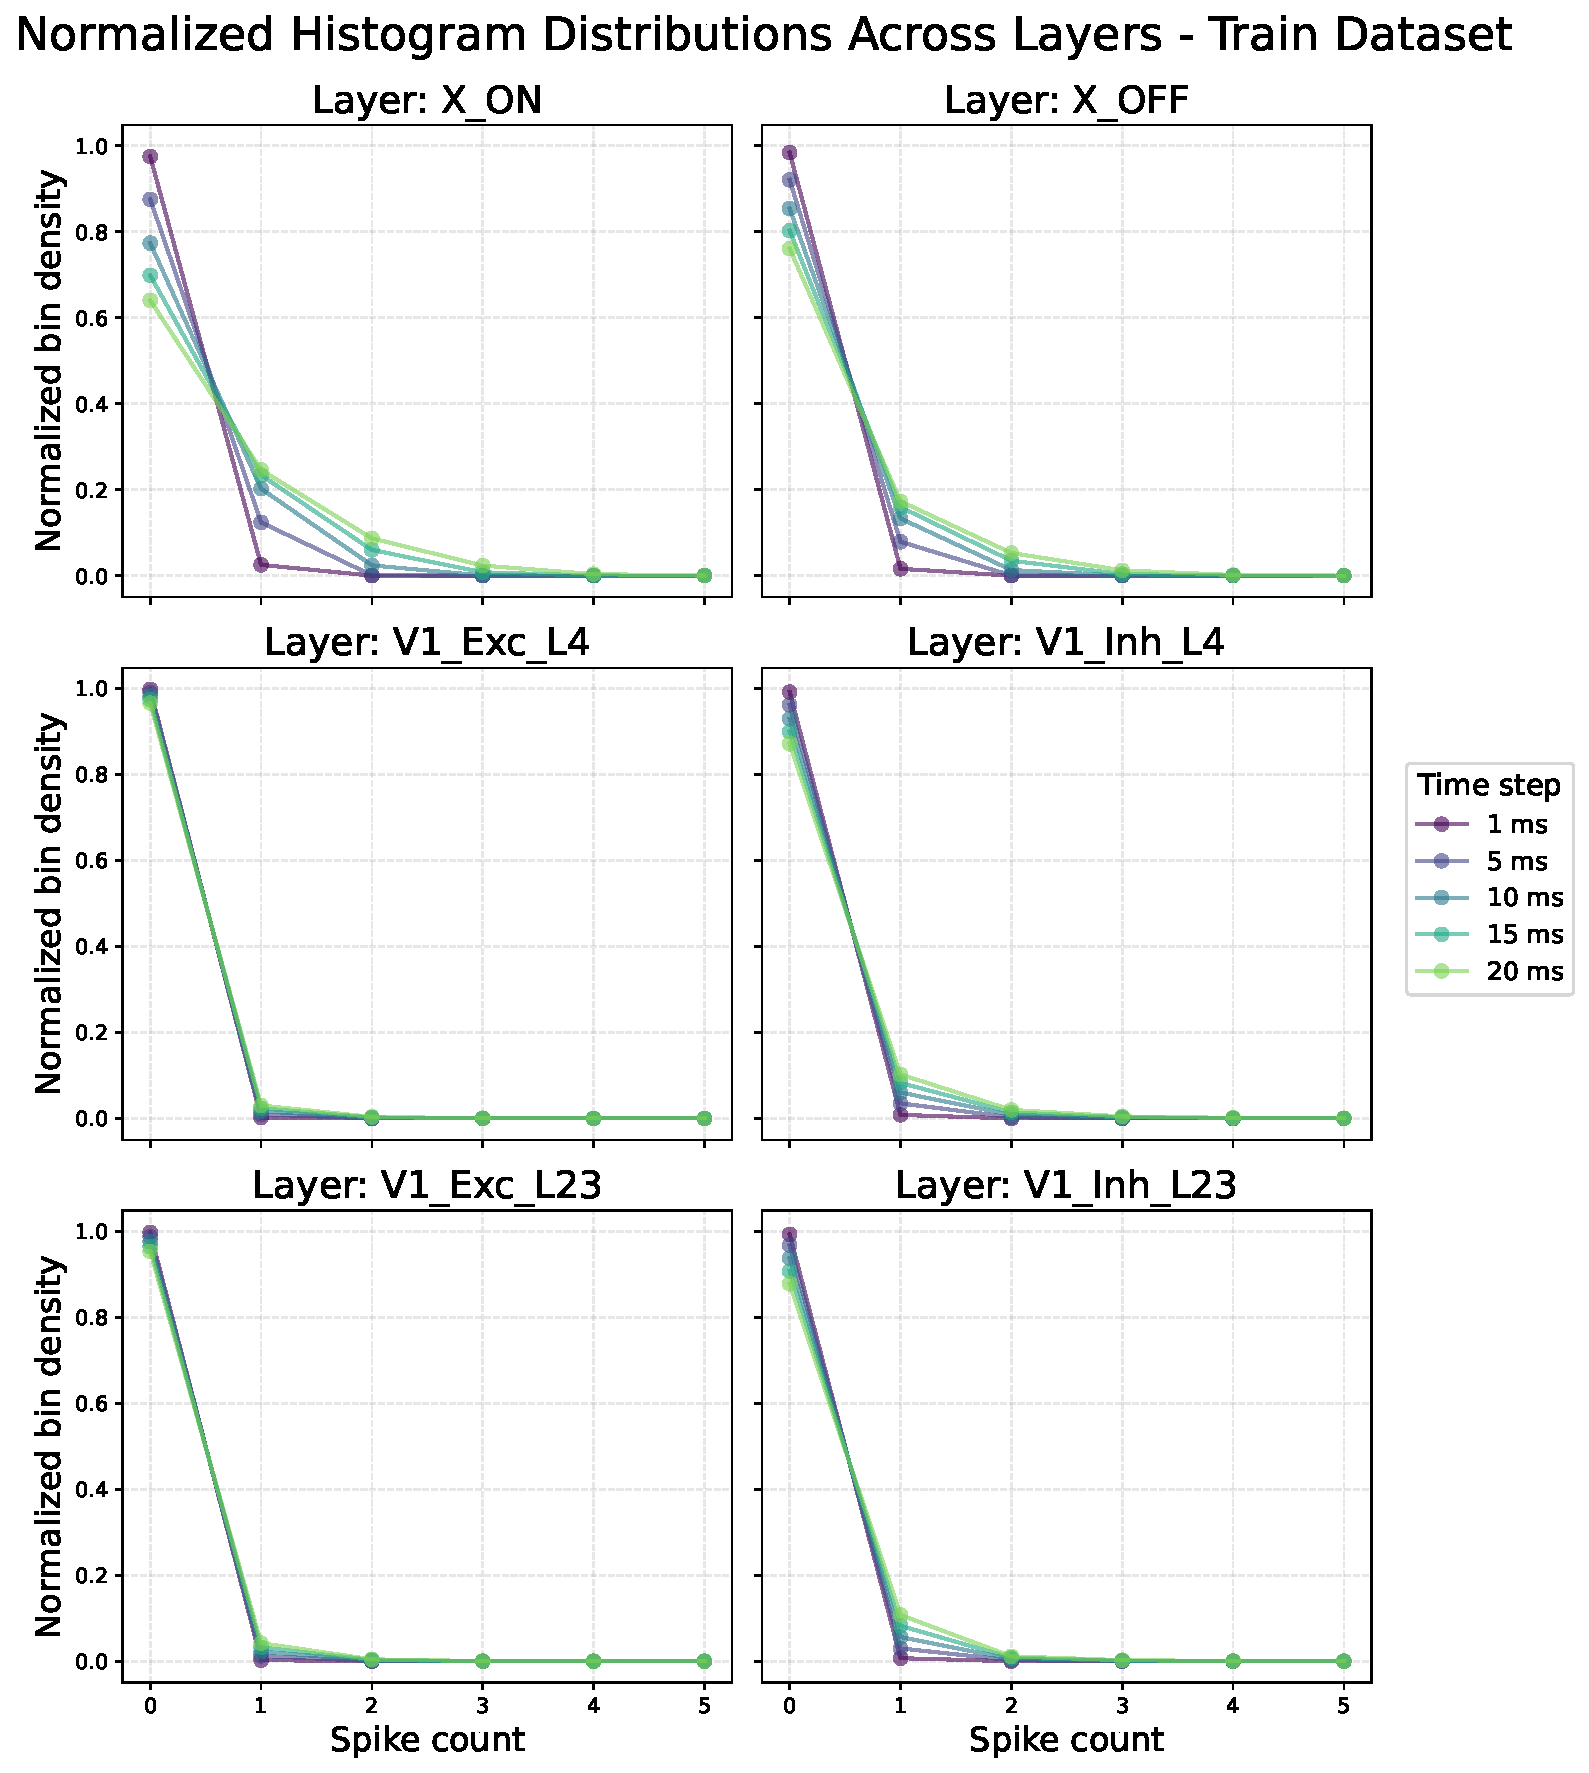
\includegraphics[width=\linewidth]{img/plots/time_step_counts_train.pdf}
    \caption{Evolution of spike counts per time bin with increasing bin size across all neuronal populations in the train dataset.}
    \label{fig:spike_count_distribution_train}
\end{figure}

\begin{figure}
    \centering
    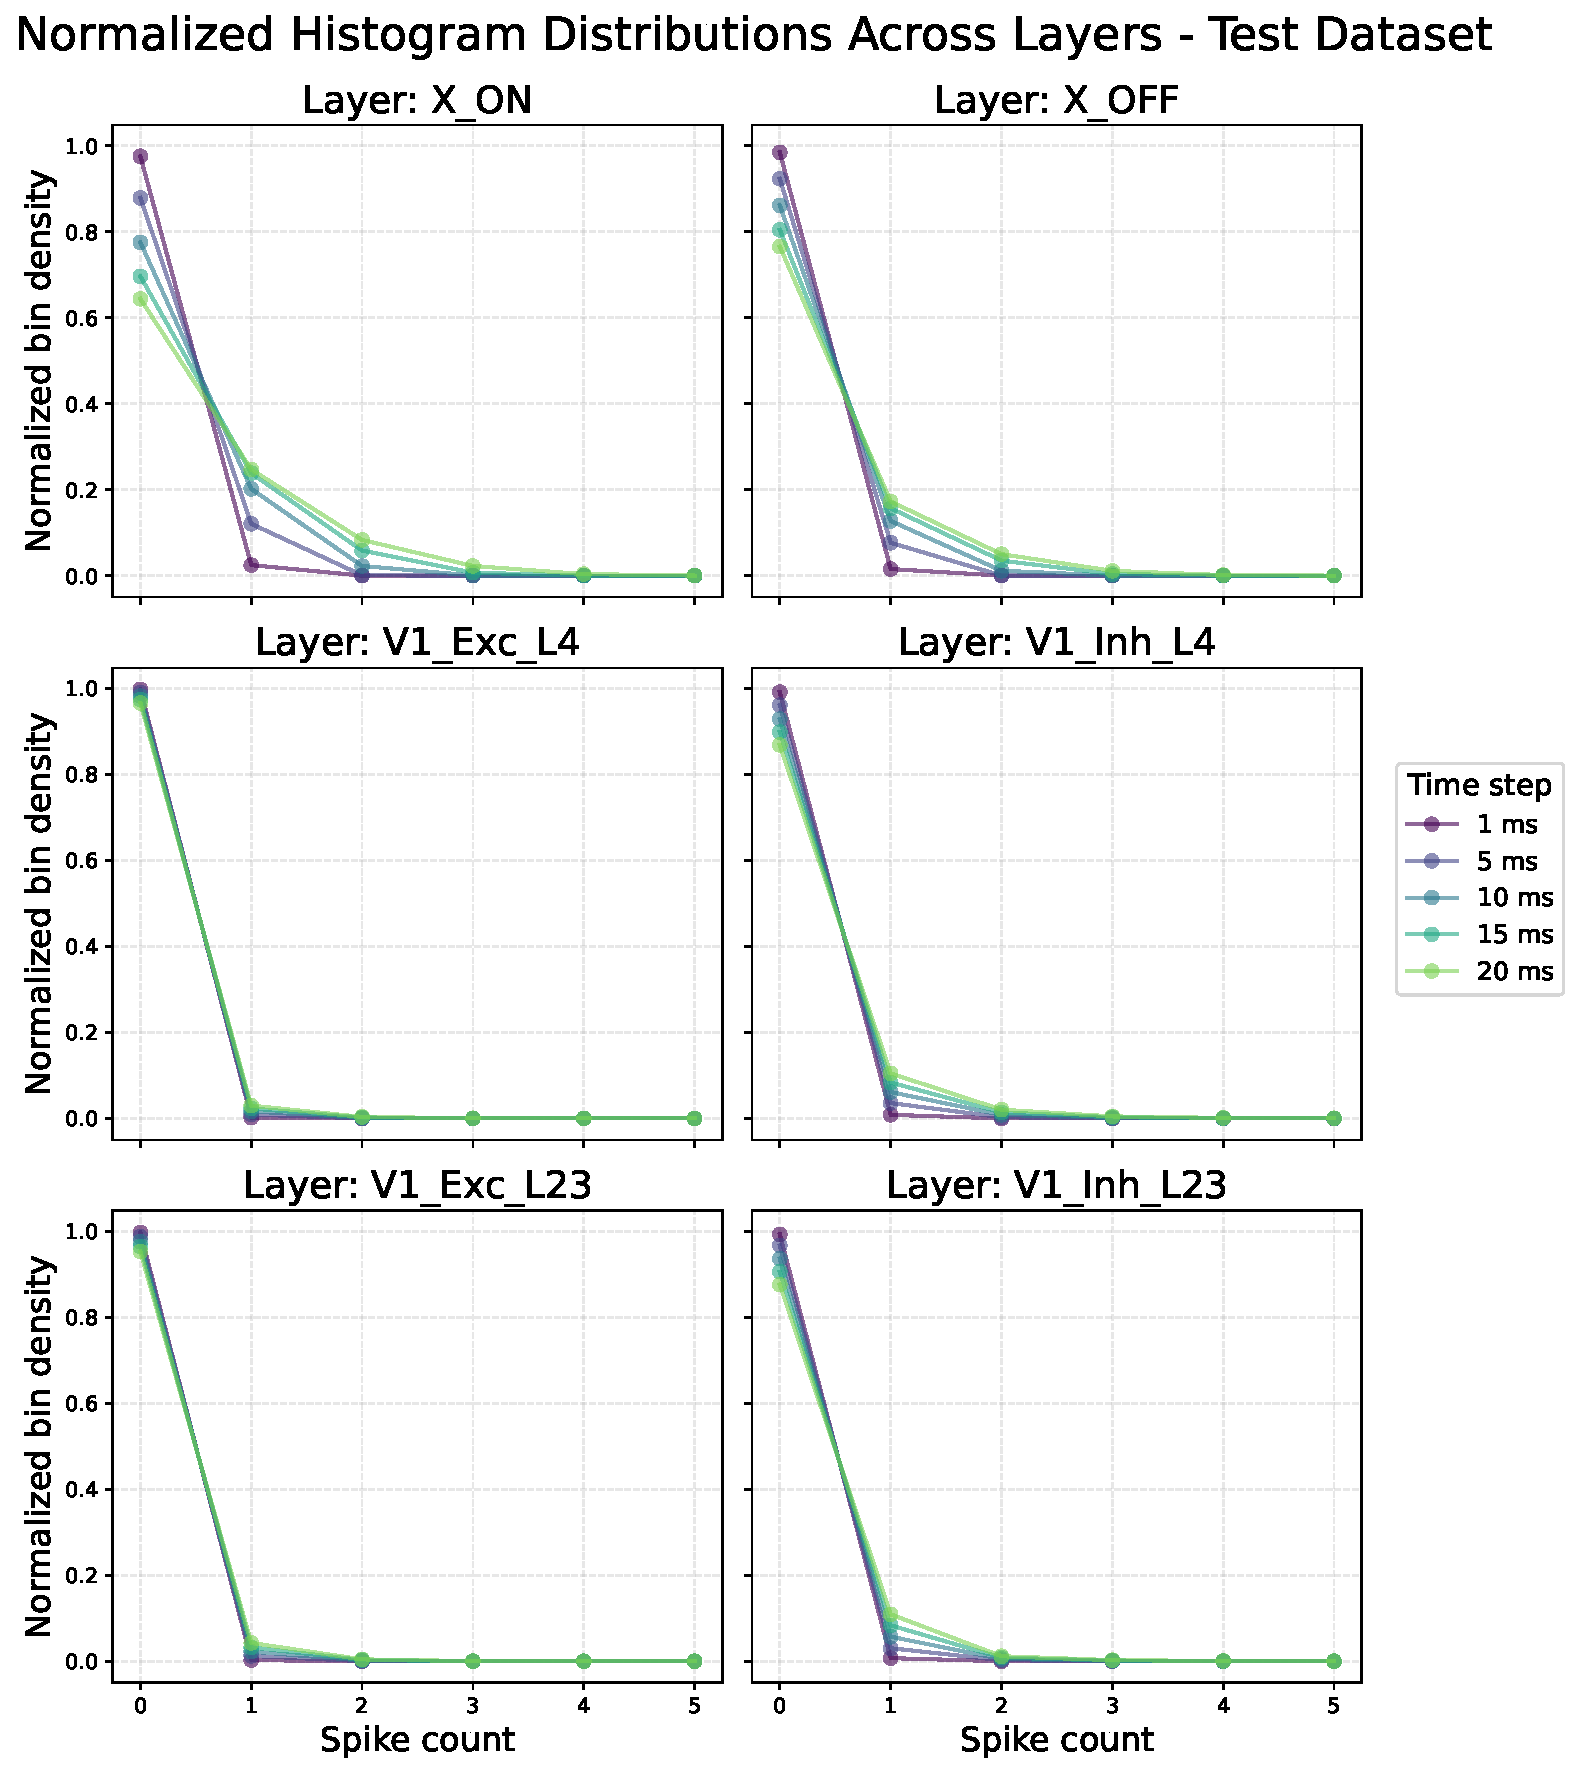
\includegraphics[width=\linewidth]{img/plots/time_step_counts_test.pdf}
    \caption{Evolution of spike counts per time bin with increasing bin size across all neuronal populations in the test dataset.}
    \label{fig:spike_count_distribution_test}
\end{figure}


\subsubsection{Spike Count Distribution Across Time}
\label{subsubsec:spike_time_distribution}
Next, we examine the distribution of spike counts across time for different bin sizes. We propose the following:

\begin{claim}[Temporal Spike Count Distribution]
    The temporal distribution of spike counts per experiment remains consistent across all tested bin sizes. This supports the preservation of temporal response patterns.
\end{claim}

Figures~\ref{fig:temporal_spike_distribution_train} and~\ref{fig:temporal_spike_distribution_test} show the mean spike counts over time for all neuronal populations in the training and test datasets, respectively. These distributions were interpolated to the 1~ms time scale using cubic interpolation.

\begin{figure}
    \centering
    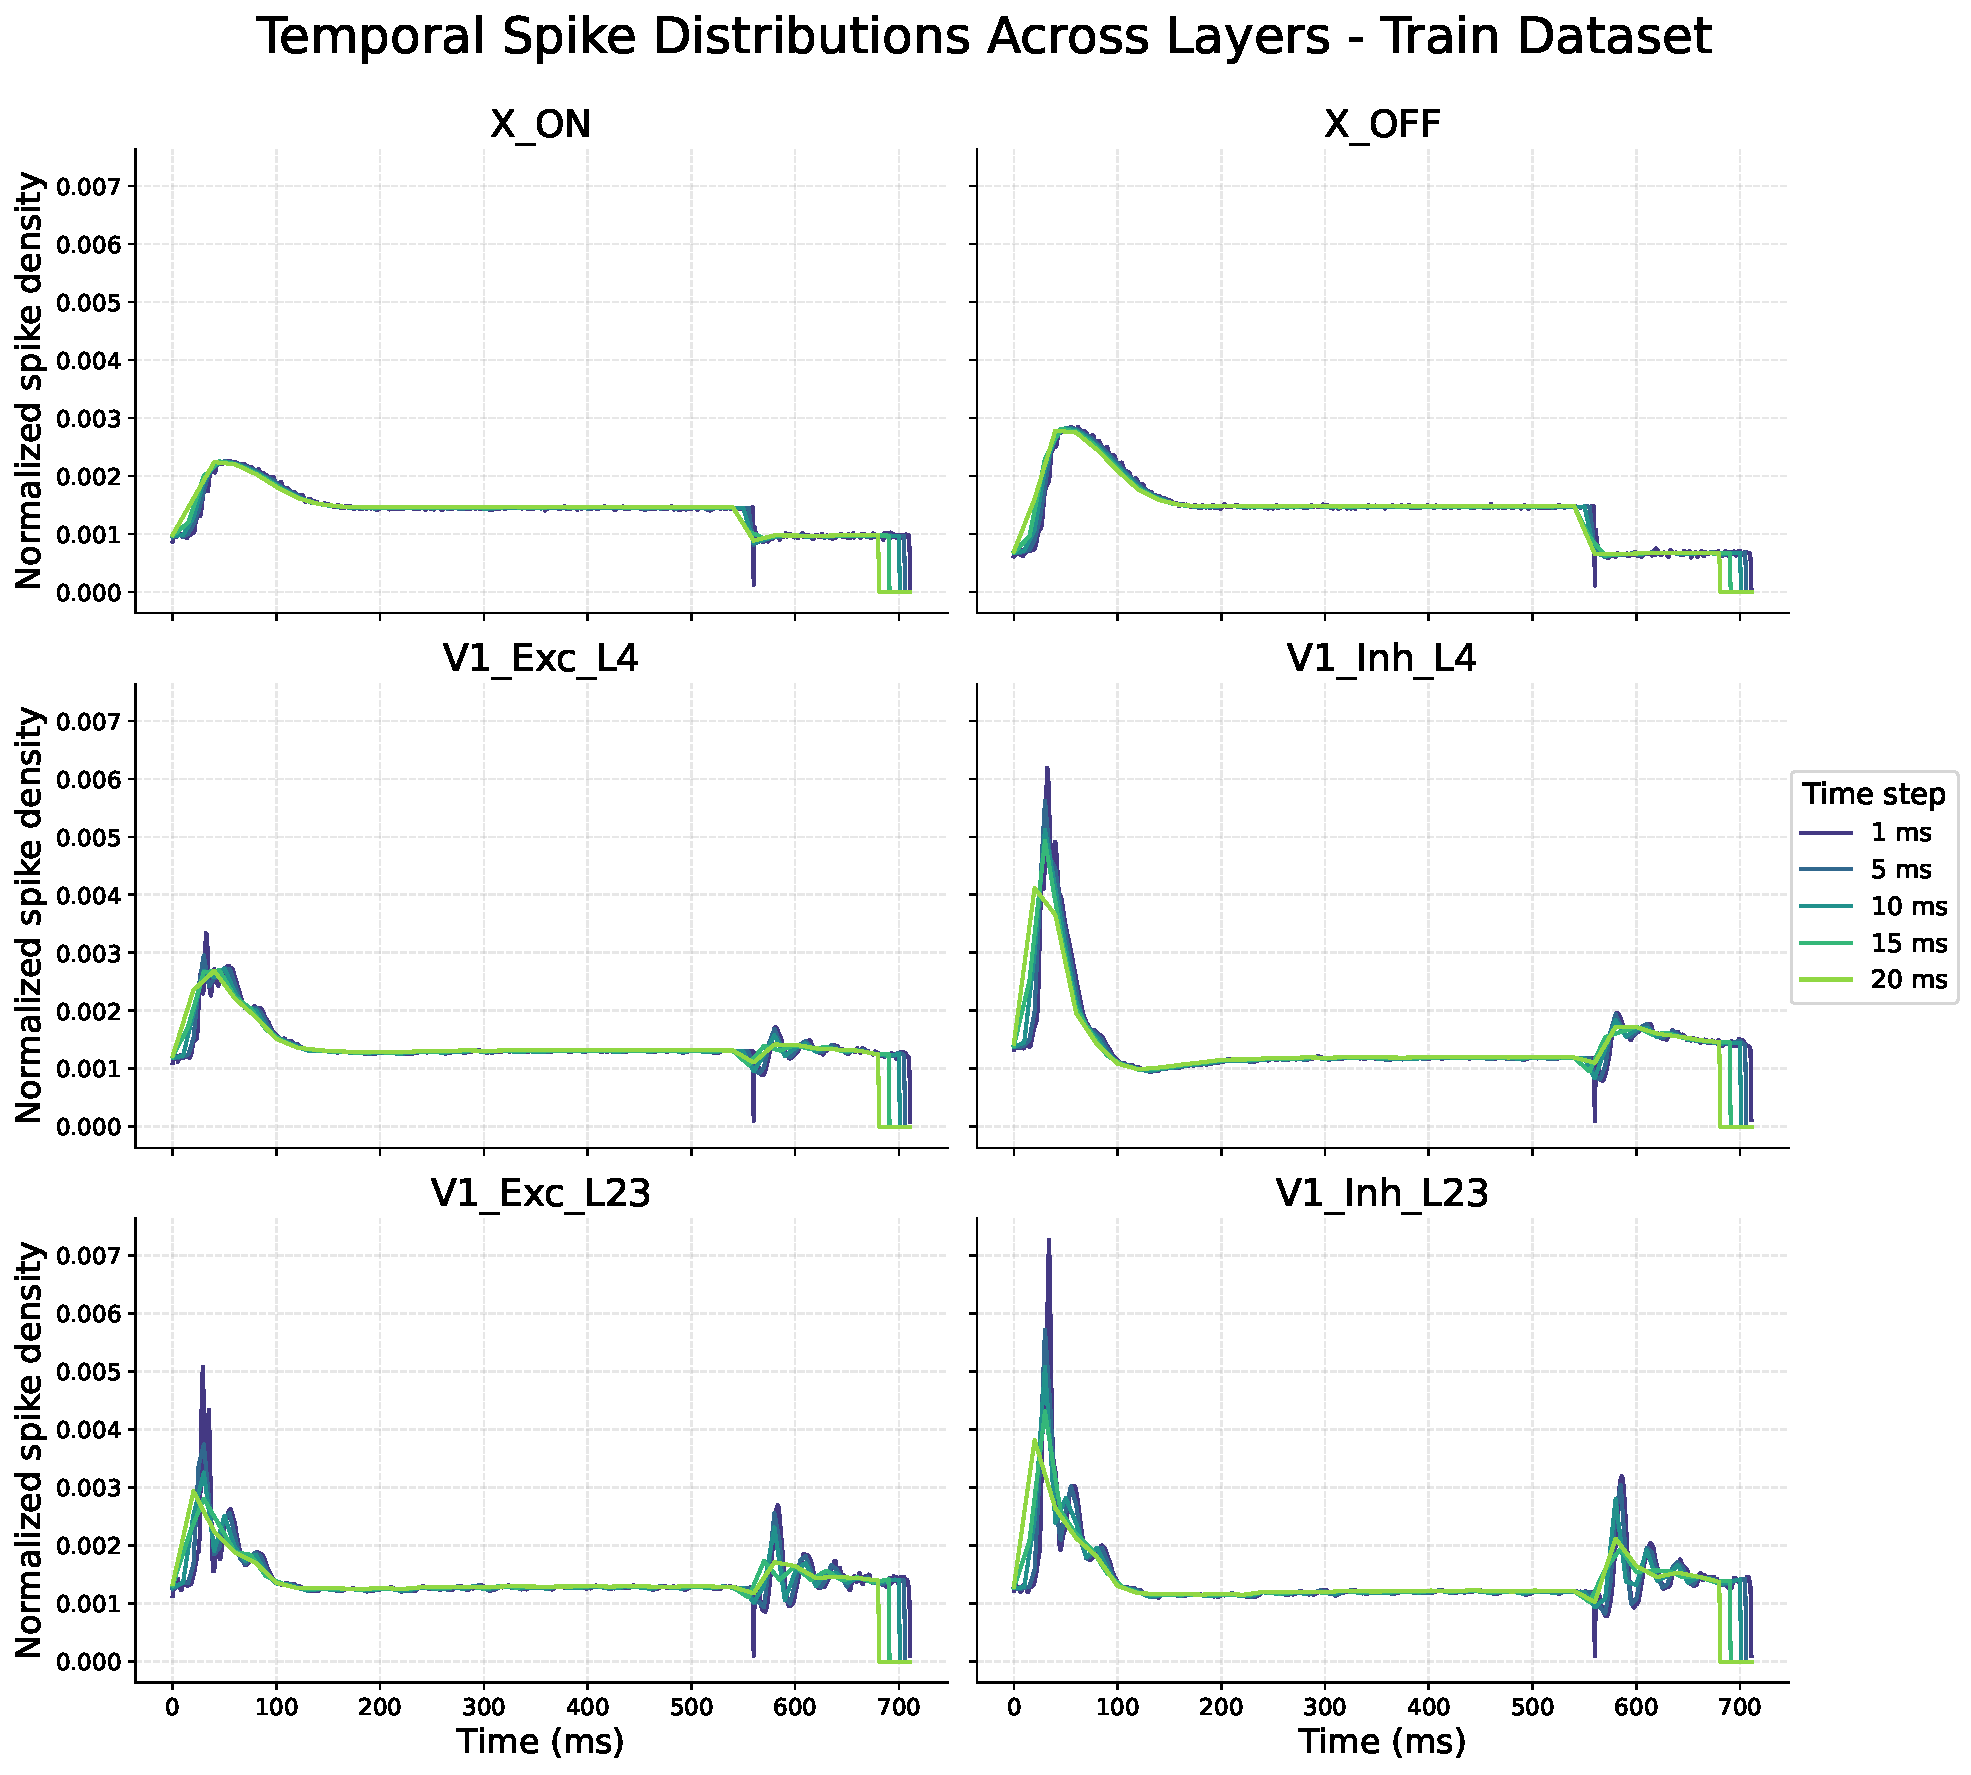
\includegraphics[width=\linewidth]{img/plots/temporal_spike_distribution_train.pdf}
    \caption{Comparison of temporal spike count distributions for different time bin sizes across all neuronal populations in the train dataset. The curves are interpolated to the original 1~ms resolution using cubic interpolation to improve line smoothness.}
    \label{fig:temporal_spike_distribution_train}
\end{figure}

\begin{figure}
    \centering
    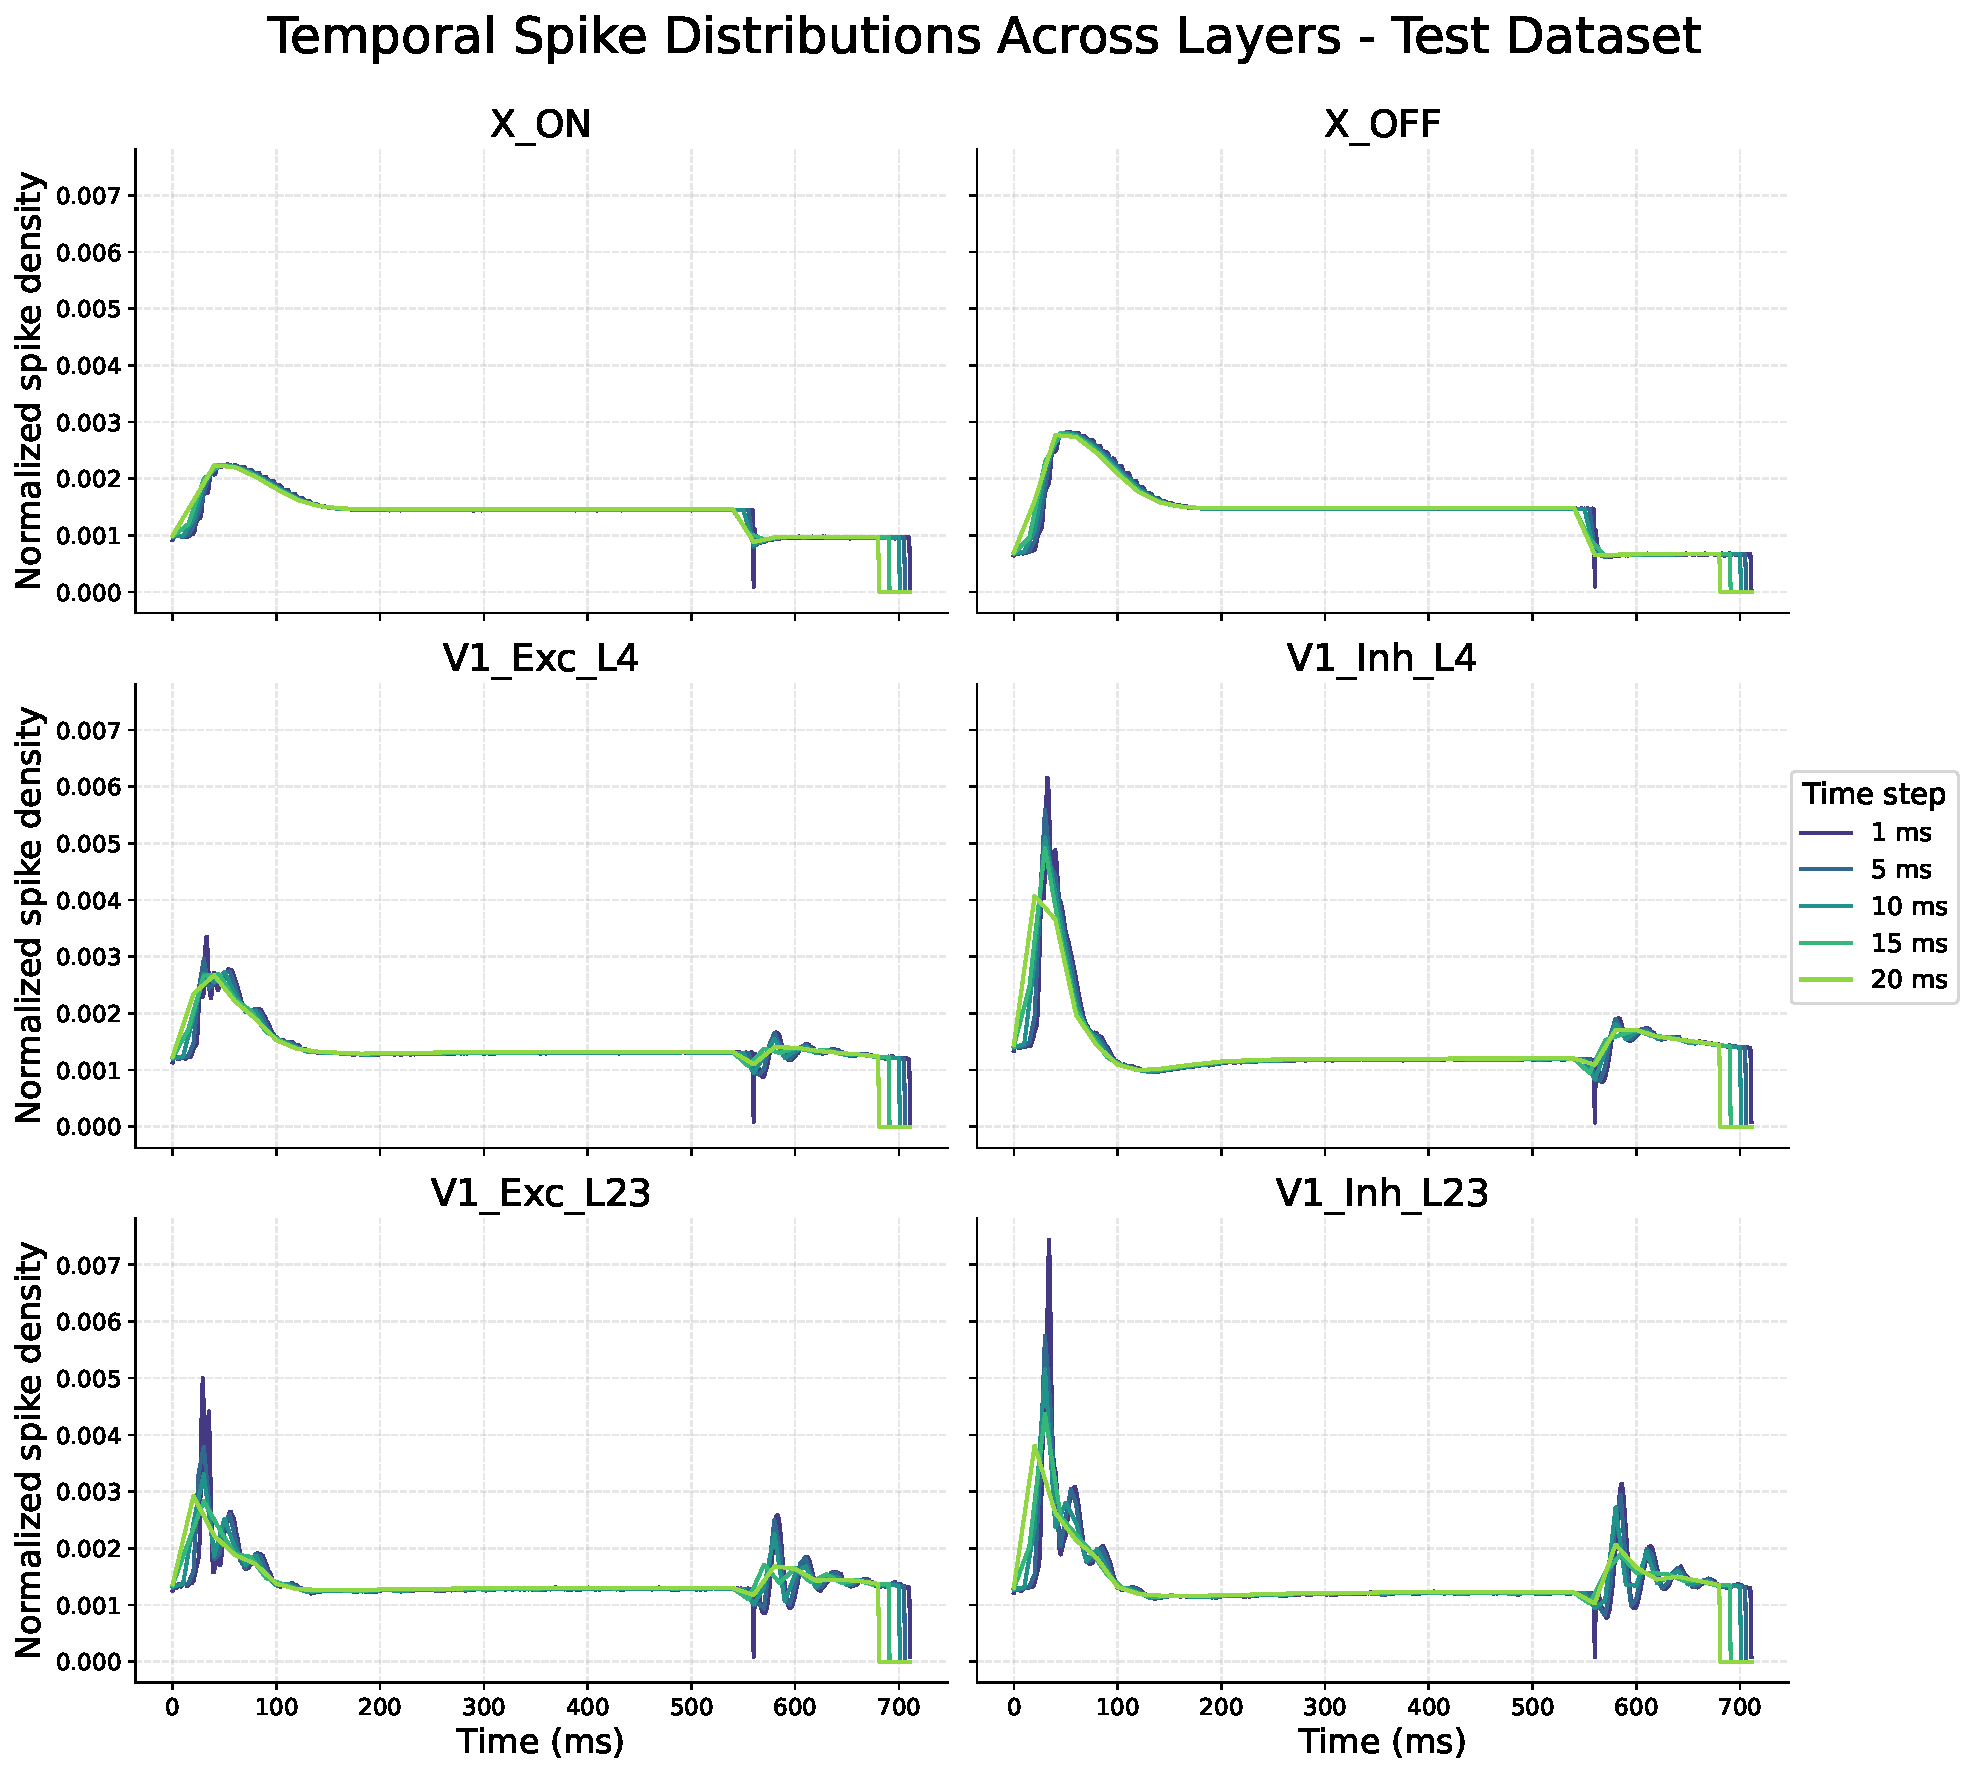
\includegraphics[width=\linewidth]{img/plots/temporal_spike_distribution_test.pdf}
    \caption{Comparison of temporal spike count distributions for different time bin sizes across all neuronal populations in the test dataset. The curves are interpolated to the original 1~ms resolution using cubic interpolation to improve line smoothness.}
    \label{fig:temporal_spike_distribution_test}
\end{figure}

These plots show a clear reduction in noise with increasing bin size, particularly in excitatory layers. The training dataset appears noisier than the test set, likely due to the test set's smaller size and the averaging effect of multiple trials per experiment.

Importantly, the overall distribution shape is preserved across bin sizes. This indicates that binning effectively reduces noise without substantially altering temporal dynamics. Heatmaps in Figure~\ref{fig:correlation_time_bin_size} display Pearson correlation coefficients across different bin sizes, confirming strong similarity in spike distributions over time.

\begin{figure}
    \centering
    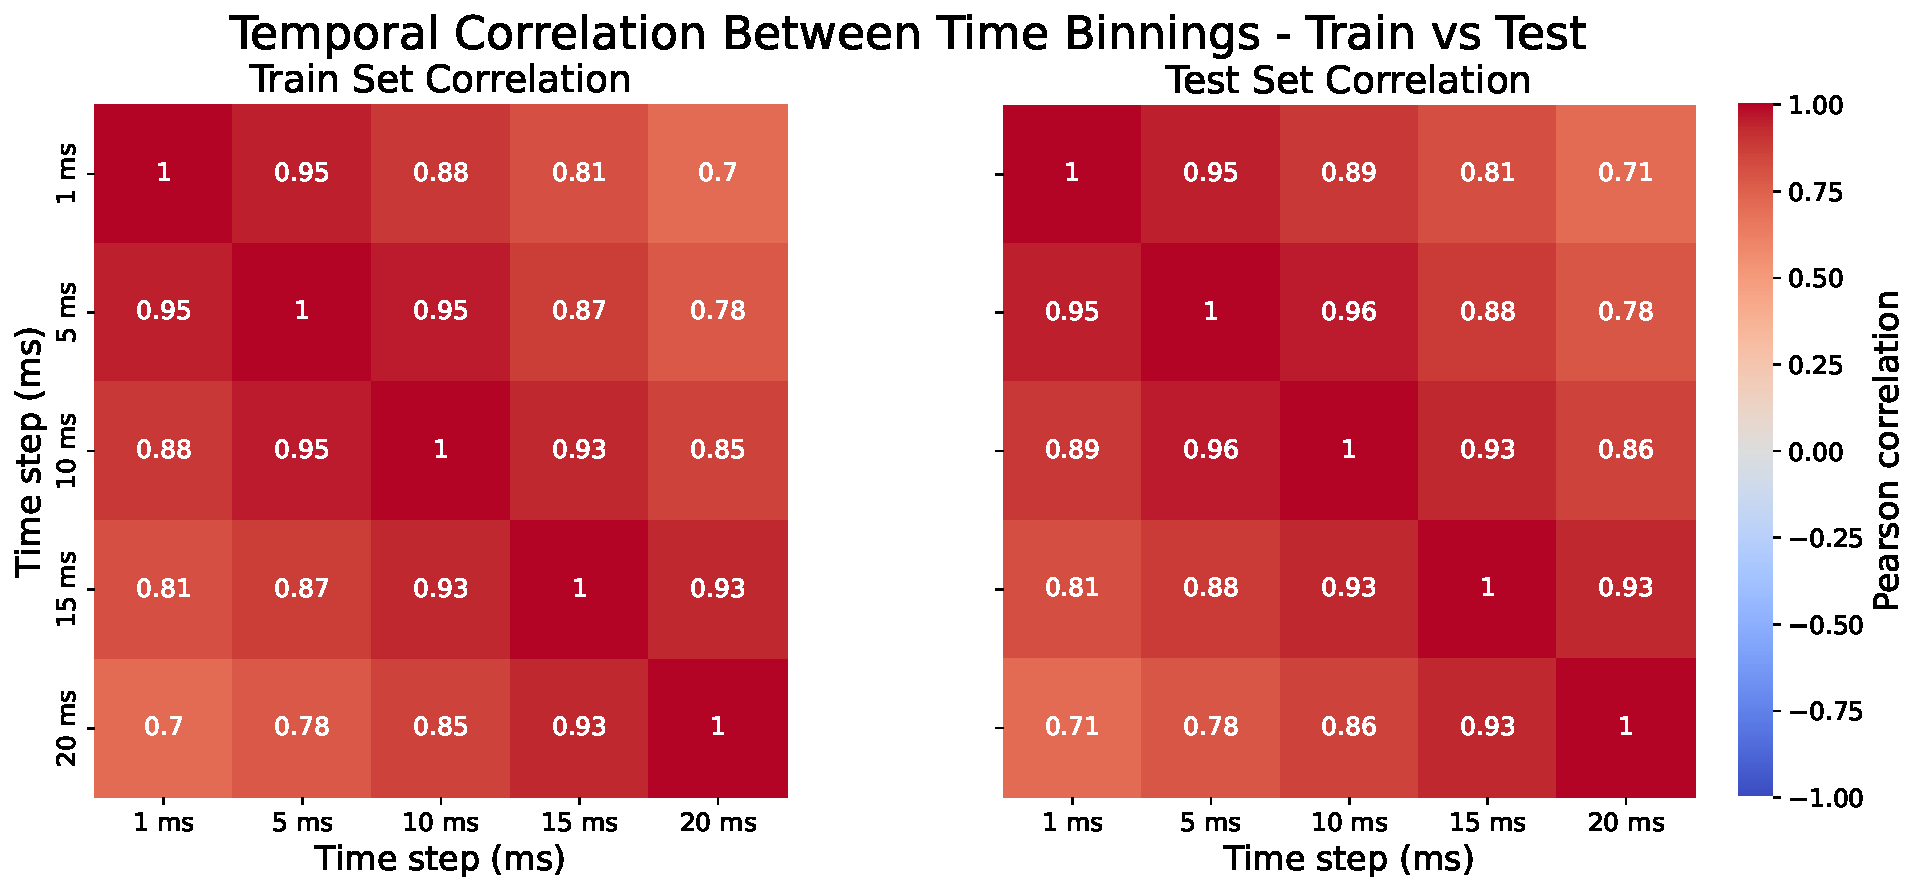
\includegraphics[width=\linewidth]{img/plots/temporal_correlation_time_bin_size.pdf}
    \caption{Heatmaps of Pearson correlation coefficients for spike count distributions over time between different time bin sizes in the train and test datasets.}
    \label{fig:correlation_time_bin_size}
\end{figure}

\subsubsection{Synchrony of Neuronal Populations in Different Time Bins}
\label{subsubsec:neuron_synchrony_binning}

Lastly, we evaluate how time binning affects synchrony, the proportion of neurons firing simultaneously within the same time bin. Synchrony provides insight into the collective temporal dynamics of neuronal populations and is widely studied in neuroscience (\citet{Singer1999}).

Our analysis focuses on the mean synchrony across all time steps. We state the following:

\begin{claim}[Synchrony of Neuronal Populations Across Time Bins]
    The mean synchrony of neuronal populations remains consistent across different time bin sizes. This implies that temporal structure of the dataset is largely preserved.
\end{claim}
\label{claim:synchrony_time_bins_size}

Figures~\ref{fig:boxplot_synchrony_time_train} and~\ref{fig:boxplot_synchrony_time_test} show synchrony distributions for each layer in the training and test datasets. Tables~\ref{tab:synchrony_time_bins_summary_train} and~\ref{tab:synchrony_time_bins_summary_test} summarize the mean and variance of synchrony values.

\begin{figure}
    \centering
    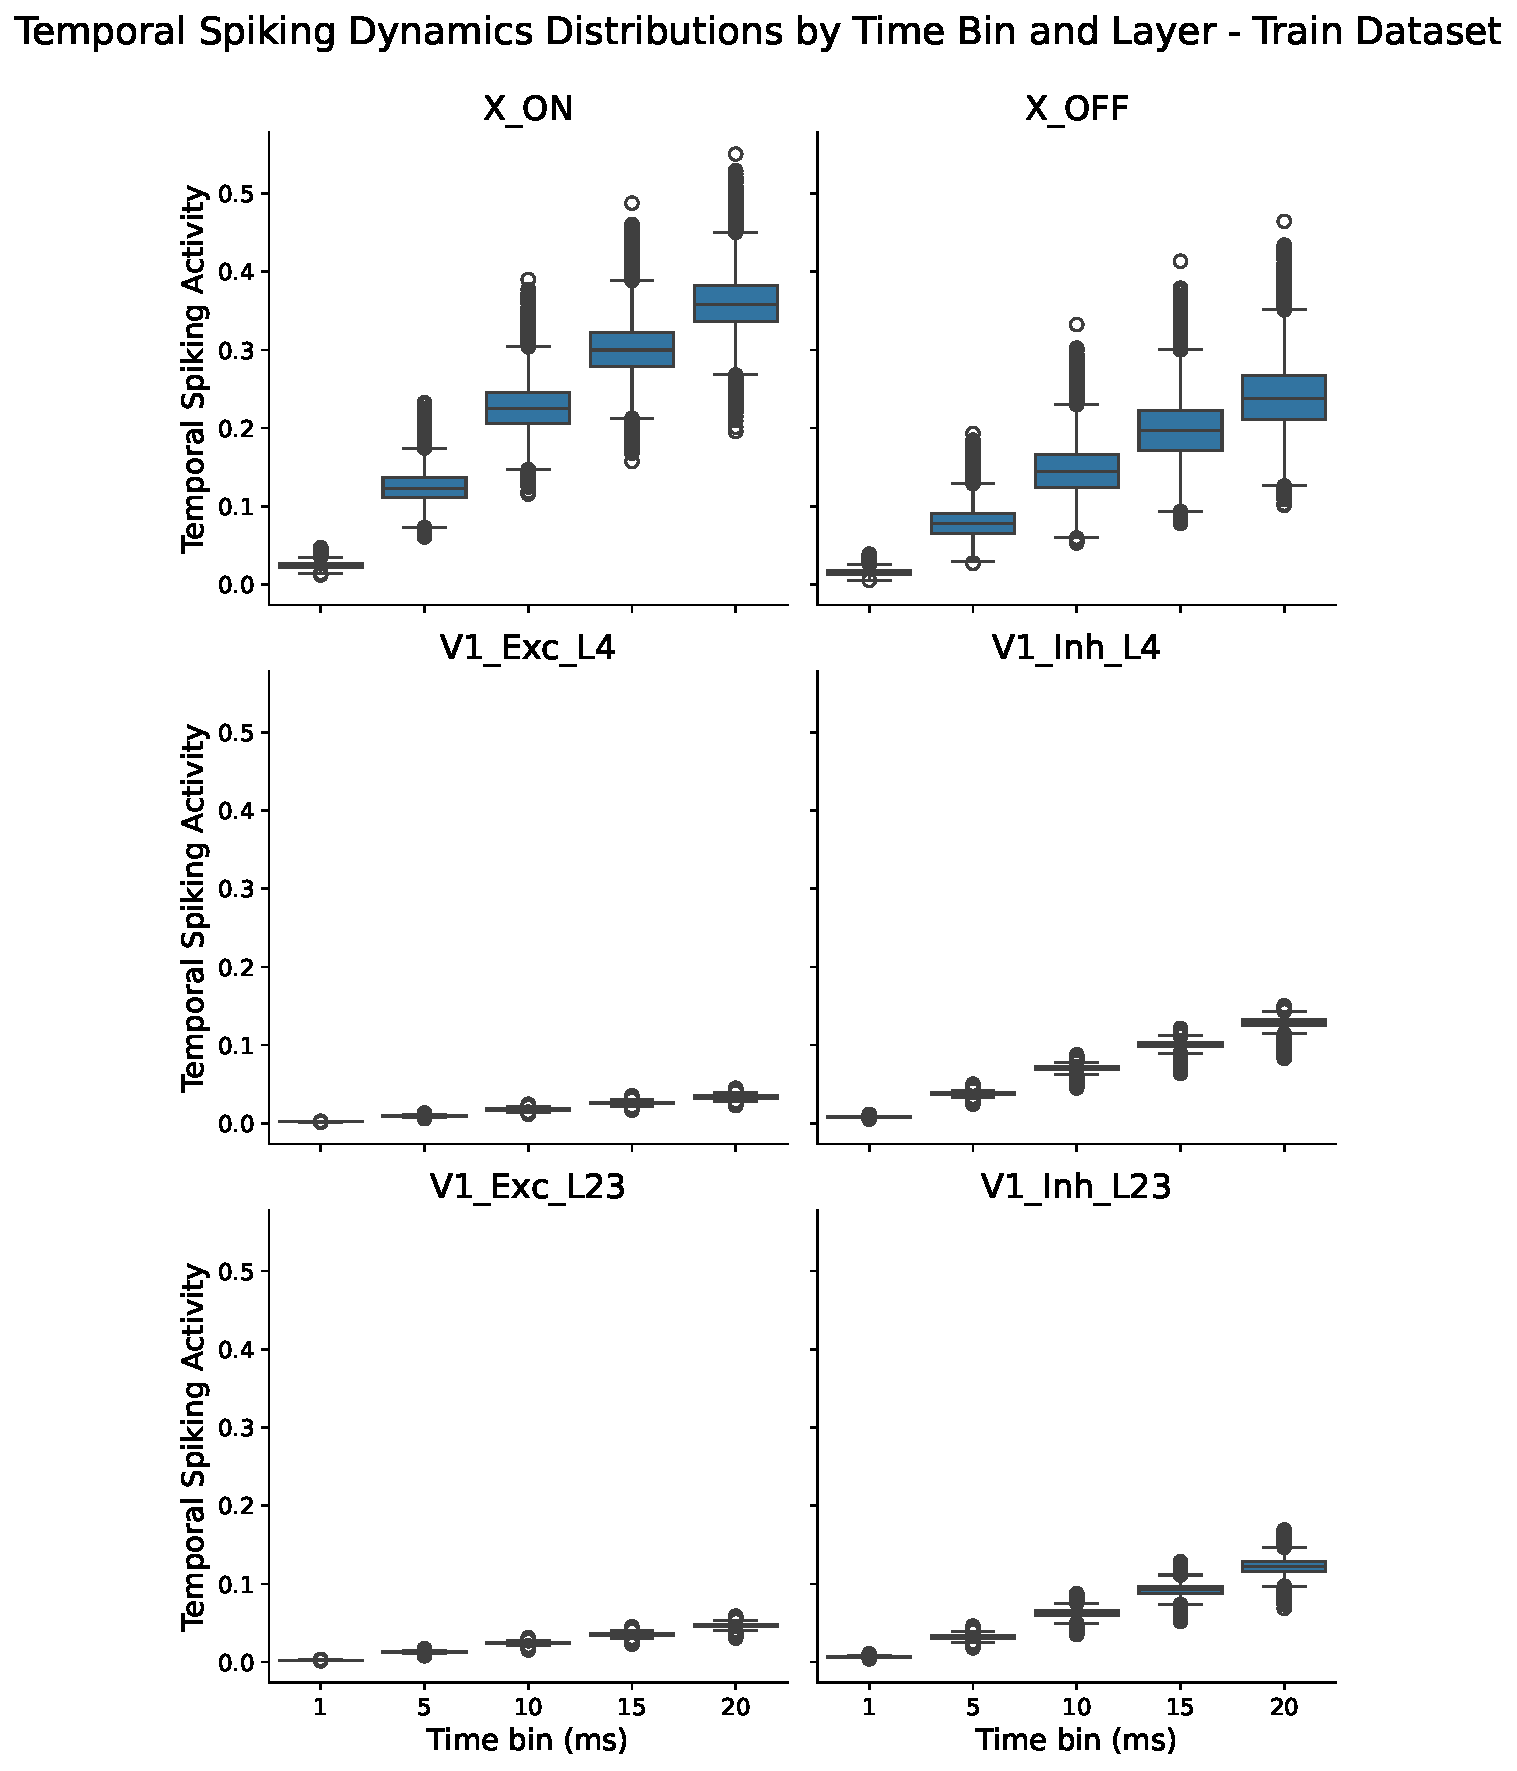
\includegraphics[width=0.92\linewidth]{img/plots/synchrony_boxplot_time_bins_train.pdf}
    \caption{Distribution of mean population synchrony across different time bin sizes for all neuronal populations in the train dataset. The boxplot represents the distribution of mean synchrony values calculated across all experiments}
    \label{fig:boxplot_synchrony_time_train}
\end{figure}


\begin{figure}
    \centering
    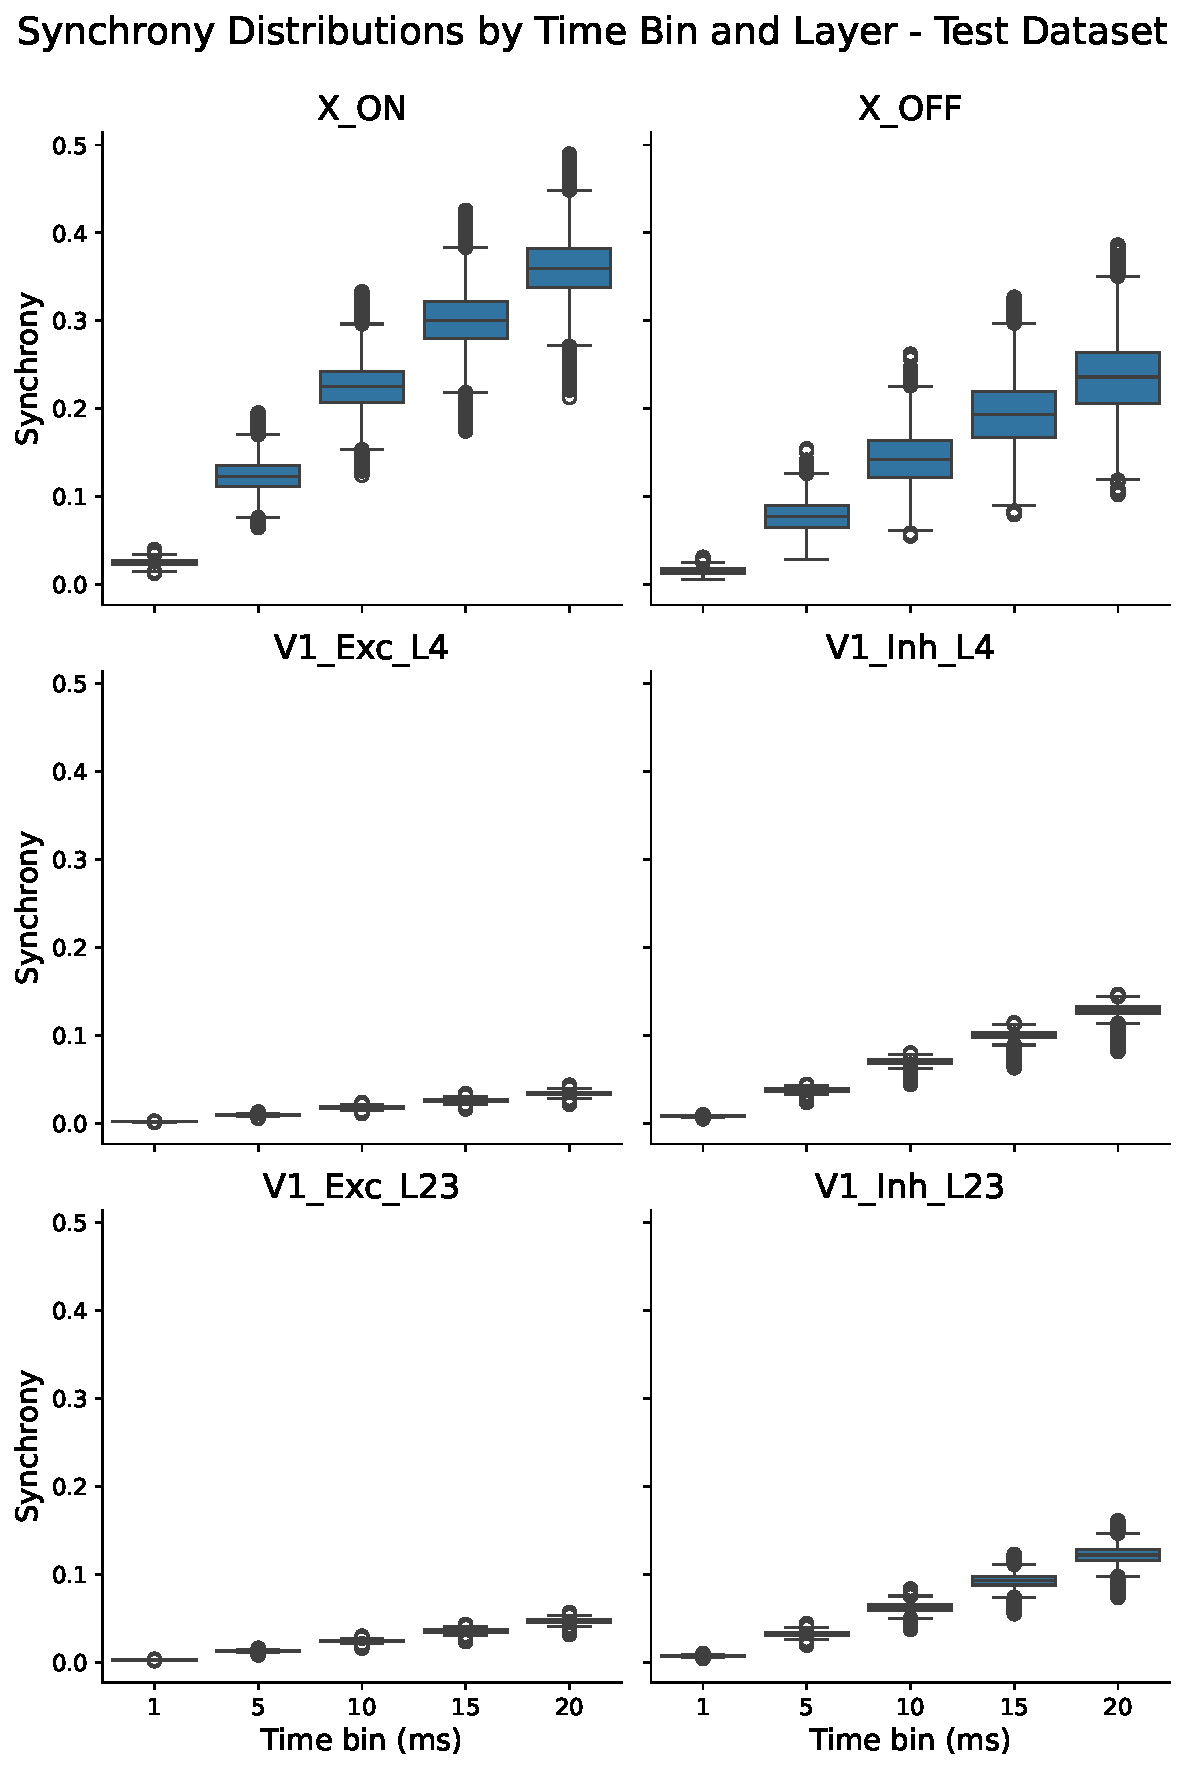
\includegraphics[width=0.92\linewidth]{img/plots/synchrony_boxplot_time_bins_test.pdf}
    \caption{Distribution of mean population synchrony across different time bin sizes for all neuronal populations in the test dataset. The boxplot represents the distribution of mean synchrony values calculated across all experiments}
    \label{fig:boxplot_synchrony_time_test}
\end{figure}

\begin{table}
    \centering\footnotesize\sf
    \begin{tabular}{lrr}
    \toprule
    time step & mean & variance \\
    \midrule
    1 & 0.0101 & 0.0001 \\
    5 & 0.0494 & 0.0018 \\
    10 & 0.0912 & 0.0057 \\
    15 & 0.1256 & 0.0098 \\
    20 & 0.1551 & 0.0134 \\
    \addlinespace % a nice non-intrusive separator of data groups (or final table sums)
    \bottomrule
    \end{tabular}
    \caption{\textbf{Summary of synchrony statistics across time bin sizes in the train dataset:} This table reports the mean and variance of population synchrony across all layers for each time bin size.}
    \label{tab:synchrony_time_bins_summary_train}
\end{table}

\begin{table}
    \centering\footnotesize\sf
    \begin{tabular}{lrr}
    \toprule
    time step & mean & variance \\
    \midrule
    1 & 0.0101 & 0.0001 \\
    5 & 0.0491 & 0.0017 \\
    10 & 0.0908 & 0.0057 \\
    15 & 0.1250 & 0.0097 \\
    20 & 0.1545 & 0.0133 \\
    \addlinespace % a nice non-intrusive separator of data groups (or final table sums)
    \bottomrule
    \end{tabular}
    \caption{\textbf{Summary of synchrony statistics across time bin sizes in the test dataset:} This table reports the mean and variance of population synchrony across all layers for each time bin size.}
    \label{tab:synchrony_time_bins_summary_test}
\end{table}

Synchrony increases with larger time bins, reflecting a higher likelihood of coincident spiking. This effect is most pronounced in LGN layers, especially X\_ON, while V1 excitatory layers show a milder change. These findings suggest that while synchrony is affected by bin size, the overall temporal dynamics are preserved.

We conclude that a bin size of 20~ms strikes a practical balance between maintaining temporal fidelity, minimizing data noise, and ensuring computational efficiency.


\subsection{Model Subset Selection Analysis}
\label{subsec:subset_selection_analysis}

In this section, we analyze the impact of selecting a subset of neurons from the original SNN model. As discussed in Section~\ref{subsubsec:subset_selection}, we selected only 10\% of the neurons due to memory constraints and the computational demands of model training. Our primary interest lies in assessing how this subset selection affects the temporal properties of the dataset, which are central to our research.

All experiments in this section are conducted on the dataset with a 20~ms time bin size (as used in our model) and focus on the training dataset unless stated otherwise. As shown previously in Section~\ref{subsubsec:time_bins_merging}, the results from the training and test datasets are largely consistent.

\subsubsection{Total Spike Counts Across Time Bins}
\label{subsubsec:total_spike_counts_subset}
We begin by analyzing the distribution of spike counts in the time bins for the full dataset and for the subset datasets. Table~\ref{tab:subset_spike_count_distribution} summarizes the mean spike count ratios across all model subsets compared to the full dataset.

\begin{table}
    \centering\footnotesize\sf
    \begin{tabular}{rrrr}
        \toprule
        Spike Count & Full Dataset Ratio & Subsets Mean Ratio & Subsets Standard Deviation \\
        \midrule
        0 & 0.9105 & 0.9102 & 0.0004 \\
        1 & 0.0710 & 0.0712 & 0.0003 \\
        2 & 0.0147 & 0.0148 & 0.0001 \\
        3 & 0.0032 & 0.0032 & 0.0000 \\
        4 & 0.0005 & 0.0005 & 0.0000 \\
        5 & 0.0001 & 0.0001 & 0.0000 \\
        \bottomrule
    \end{tabular}
    \caption{\textbf{Comparison of spike count distributions between full and subset datasets:} This table presents the mean spike count ratios and standard deviations across all model subsets, relative to the full dataset.}
    \label{tab:subset_spike_count_distribution}
\end{table}

The table shows that the differences in spike count distributions between the full and subset datasets are minimal, with low standard deviations. This suggests that randomly selecting a subset of neurons does not significantly impact the overall spike count distribution.

\subsubsection{Spike Count Distribution Across Time}
\label{subsubsec:spike_time_distribution_subset}

Next, we compare the temporal spike count distributions of the subset datasets with that of the full dataset. Figure~\ref{fig:temporal_distribution_subset_vs_full_train} shows the mean temporal behavior across layers for both the full dataset and the average of all subsets. The shaded area represents the standard deviation across subsets.
\begin{figure}
    \centering
    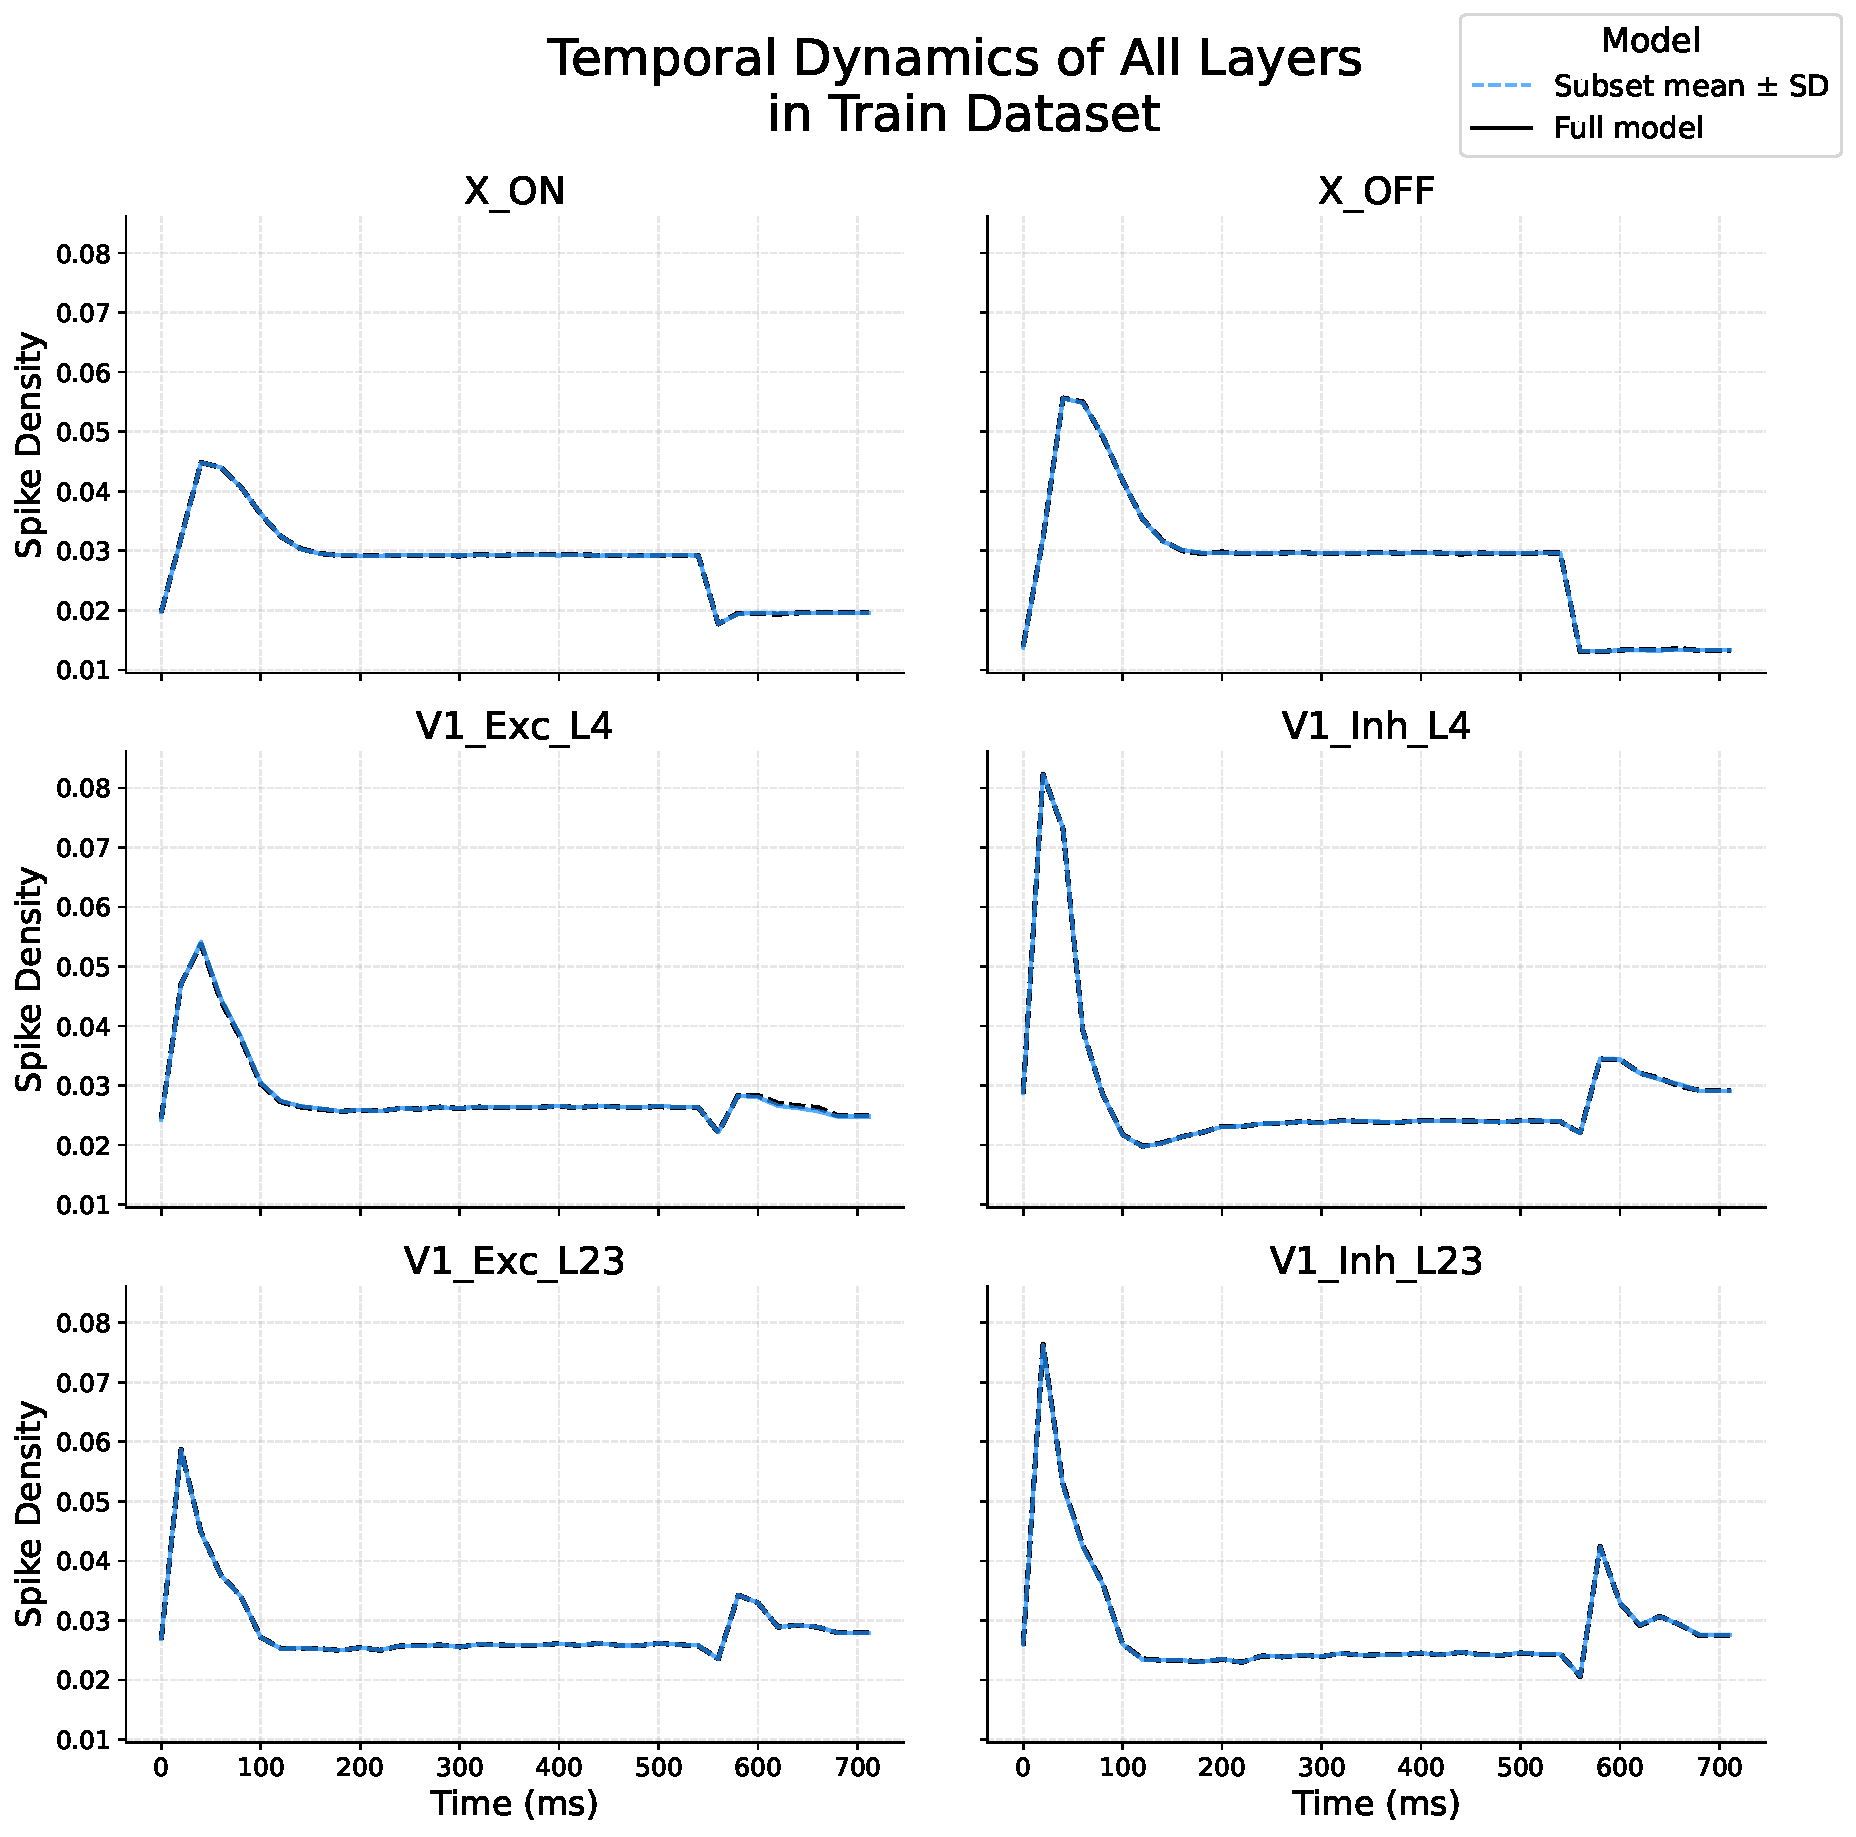
\includegraphics[width=\linewidth]{img/plots/temporal_distribution_subset_vs_full_train.pdf}
    \caption{Comparison of mean temporal activity across layers for the full dataset and the average of all subsets. The shaded area indicates the standard deviation across subsets, which is very small and therefore barely visible in the plot.}
    \label{fig:temporal_distribution_subset_vs_full_train}
\end{figure}

The plot demonstrates that the mean temporal patterns of the subsets closely match those of the full dataset. The small standard deviation further confirms that the temporal properties are preserved despite the neuron subset selection.


\subsubsection{Synchrony of Neuronal Populations in Subsets}
\label{subsubsec:neuron_synchrony_subset}
Finally, we assess the effect of subset selection on neuronal synchrony. Since we are using only a portion of the neurons from the full model, it is possible that groups of neurons that typically spike together may be disrupted, potentially affecting synchrony.

Figure~\ref{fig:boxplot_synchrony_subset} displays a boxplot and jitter plot comparing the synchrony values of the full dataset and all subsets.

\begin{figure}
    \centering
    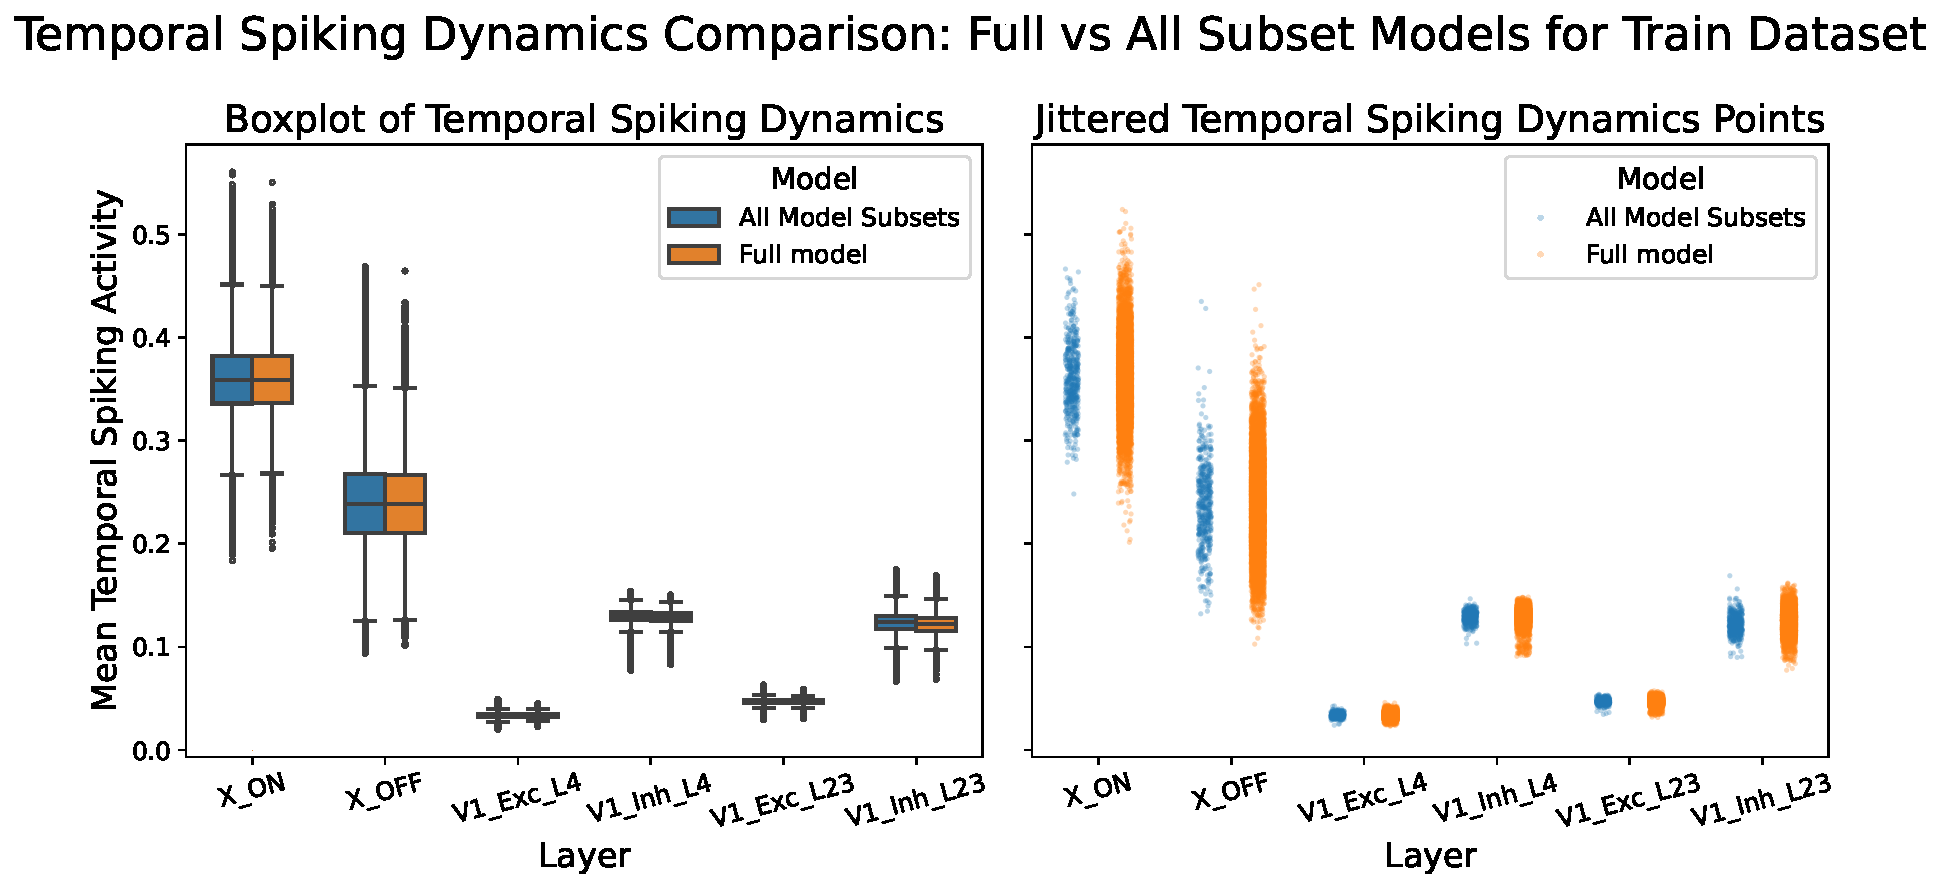
\includegraphics[width=\linewidth]{img/plots/synchrony_comparison_subset_full_train.pdf}
    \caption{Boxplot and jitter plot comparing population synchrony values between the full dataset and all subsets. Each data point represents the mean synchrony of one experiment.}
    \label{fig:boxplot_synchrony_subset}
\end{figure}

As shown, the synchrony distributions are largely similar, particularly in the excitatory layers. This aligns with earlier findings that synchrony variance was low across time bins. Although the jitter plot suggests a slightly narrower spread in the LGN layers for the subsets, the boxplots do not indicate a significant difference.

Based on these observations, we conclude that random selection of 10\% of neurons from the full SNN model does not substantially affect the dataset's statistical or temporal properties. Nevertheless, slight changes in synchrony, particularly in LGN layers, should be taken into account when interpreting model performance results.

\section{Model Evaluation}
\label{sec:model_evaluation}
In this section we focus on the evaluation of the model performance, we compare different model variants and evaluate the influence of each model additional module on the overall results. First, we focus on summary of the results and comparison of all the models based on the high level metrics. Followingly, we focus on the separate inspection of each model perfomance. At the end we focuse on the caveats of our models and try to pin point the aspects of the model that might be the cause of the prediction flaws.

If not stated differently we work with the aggregated values across 20 randomly selected neuronal populations of 10\% size of the original dataset as profoundly described in the Section~\ref{subsubsec:subset_selection}. We have selected 20 randomly chosen subsets to ideally capture the behavior of the model the best without bias caused by the model subset selection.

Throughout this section if not stated differently we will use the uniform naming of the model types that mainly build on the namings defined in the Section~
\ref{sec:model_description}. However, we also compare some model variants with slightly different setup, because of that we need to invent new naming for the differentiation of these throughout the analysis. The naming is the following. We use two simple variant models (Section~\ref{subsec:base_model_architecture}) one with tanh activation function that we note as \emph{simple (tanh)} and the second variant with leakytanh activation function (Section~\ref{subsubsec:leakytanh}) that we note as \emph{simple (leakytanh)}. Then we use only one varian of both \emph{dnn joint} (Section~\ref{subsubsec:dnn_neuron}) and \emph{dnn separate} (Section~\ref{subsubsec:dnn_separate}) for these we keep the naming as it was before. The we use 2 rnn separate (Section~\ref{subsubsec:rnn_neuron_module}) models with different TBPTT time steps that we call \emph{rnn (5 steps)} and \emph{rnn (10 steps)} for either 5 or 10 TBPTT time steps used during the model training. Last model we compare is the model using synaptic depression (Section~\ref{subsubsec:synaptic_depression}) applied only on LGN connections and with 5 TBPTT time steps, this model we label as \emph{syn adapt lgn (5 steps)}. The label part "adapt" comes from the "adaptation", the naming convention for the synaptic depression module used in our model implementation, we kept this naming to facilitate the experimental processing of the data. 

During the evaluation of the model variants on 20 subsets we have used the general setup profoundly described in the Section~\ref{sec:experimental_setup} and additionally for each model variant the hyperparameter setup described in Table~\ref{tab:evaluation_setup}. These hyperparameters has been chosen mainly by the grid search of different experimental setups for each model and partly base on our empirical knowledge and experience throughout the model development. The grid search and selection of the hyperparameters will be deeply describe in the up-coming sections of the chapter.

\begin{table}
    \centering\footnotesize\sf
    \begin{tabular}{lrrrrrrrr}
        \toprule
        Model Variant & Epochs & lr & n-ls & n-nl & n-res & s-ls & s-nl & n-tbptt \\
        \midrule
        simple (tanh) & 10 & 0.000008 & - & - & - & - & - & - \\
        simple (leakytanh) & 10 & 0.000075 & - & - & - & - & - & - \\
        dnn joint & 10 & 0.000010 & 10 & 5 & True & - & - & - \\
        dnn separate & 10 & 0.000010 & 10 & 5 & True & - & - & - \\
        rnn (steps 5) & 40 & 0.000030 & 10 & 3 & True & - & - & 5 \\
        rnn (steps 10) & 40 & 0.000030 & 10 & 3 & True & - & - & 10 \\
        syn adapt lgn (steps 5) & 40 & 0.000030 & 10 & 3 & True & 10 & 2 & 5 \\
        \bottomrule
        \end{tabular}
    \caption{\textbf{Setup of the models in evaluation:} This table presents the setup of each model used in the evaluation results processing. The setup has been mainly selected by the grid search and partially by empirical selection. The columns depicts namely: "Model Variant" - variant of the model, "Epochs" - number of training epochs, "lr" - learning rate, "n-ls" - layer size of the module of neuron, "n-nl" - number of layers of the neuron module, "n-res" - flag whether the neuron module use residual connection, "s-ls" - layer size of the synaptic depression module, "s-nl" - number of layers of synaptic depression module, "n-tbptt" - number of TBPTT time steps. In case the value is not stated (symbol "-"), it is not relevant for the model.}
    \label{tab:evaluation_setup}
\end{table}

\subsection{Overall Model Types Comparison}
\label{subsec:overall_model_types_comparison}
In this section we focus on overall comparison of all model variants based on the global metrics.

First, we look at the pearson correlation coefficients and normalized cross correlations (Section~\ref{subsec:pearson_cc} and Section~\ref{subsec:normalized_cross_correlation}) comparison of each model performance. The Table~\ref{tab:model_evaluation_overview_comparison} depicts the result overview of every model variant in evaluation and Figure~\ref{fig:model_types_correlation_comparison} shows boxplot comparison of normalized cross correlation and pearson correlation coefficient values across all model subsets.

\begin{table}
    \centering\footnotesize\sf
    \begin{tabular}{lrrrrrrrr}
        \toprule
        Model Variant & N-CC (mean) & P-CC (mean) & N-CC (std) & P-CC (std) \\
        \midrule
        rnn (10 steps) & 0.9212 & 0.7500 & 0.0084 & 0.0082 \\
        rnn (5 steps) & 0.9176 & 0.7471 & 0.0103 & 0.0089 \\
        syn adapt lgn (5 steps) & 0.8935 & 0.7275 & 0.0043 & 0.0042 \\
        dnn joint & 0.8803 & 0.7168 & 0.0021 & 0.0034 \\
        simple (leakytanh) & 0.8778 & 0.7147 & 0.0014 & 0.0032 \\
        dnn separate & 0.8430 & 0.6864 & 0.0940 & 0.0766 \\
        simple (tanh) & 0.2767 & 0.2252 & 0.0400 & 0.0321 \\
        \bottomrule
    \end{tabular}
        
    \caption{\textbf{Summary of Model Performance Metrics:} This table show summary of all model variant normalized cross correlation and pearson correlation coefficients mean and standard deviations across all model subset variants. The results are sorted by the mean normalized cross correlation. The columns depicts namely: "Model Variant" - variant of the model, "N-CC (mean)" - mean of the normalized cross correlation, "P-CC (mean)" - mean of the pearson correlation coefficient, "N-CC (std)" - standard deviation of the normalized cross correlation and "P-CC (std)" - standard deviation of the pearson correlation coefficient.}
    \label{tab:model_evaluation_overview_comparison}
\end{table}

\begin{figure}
    \centering
    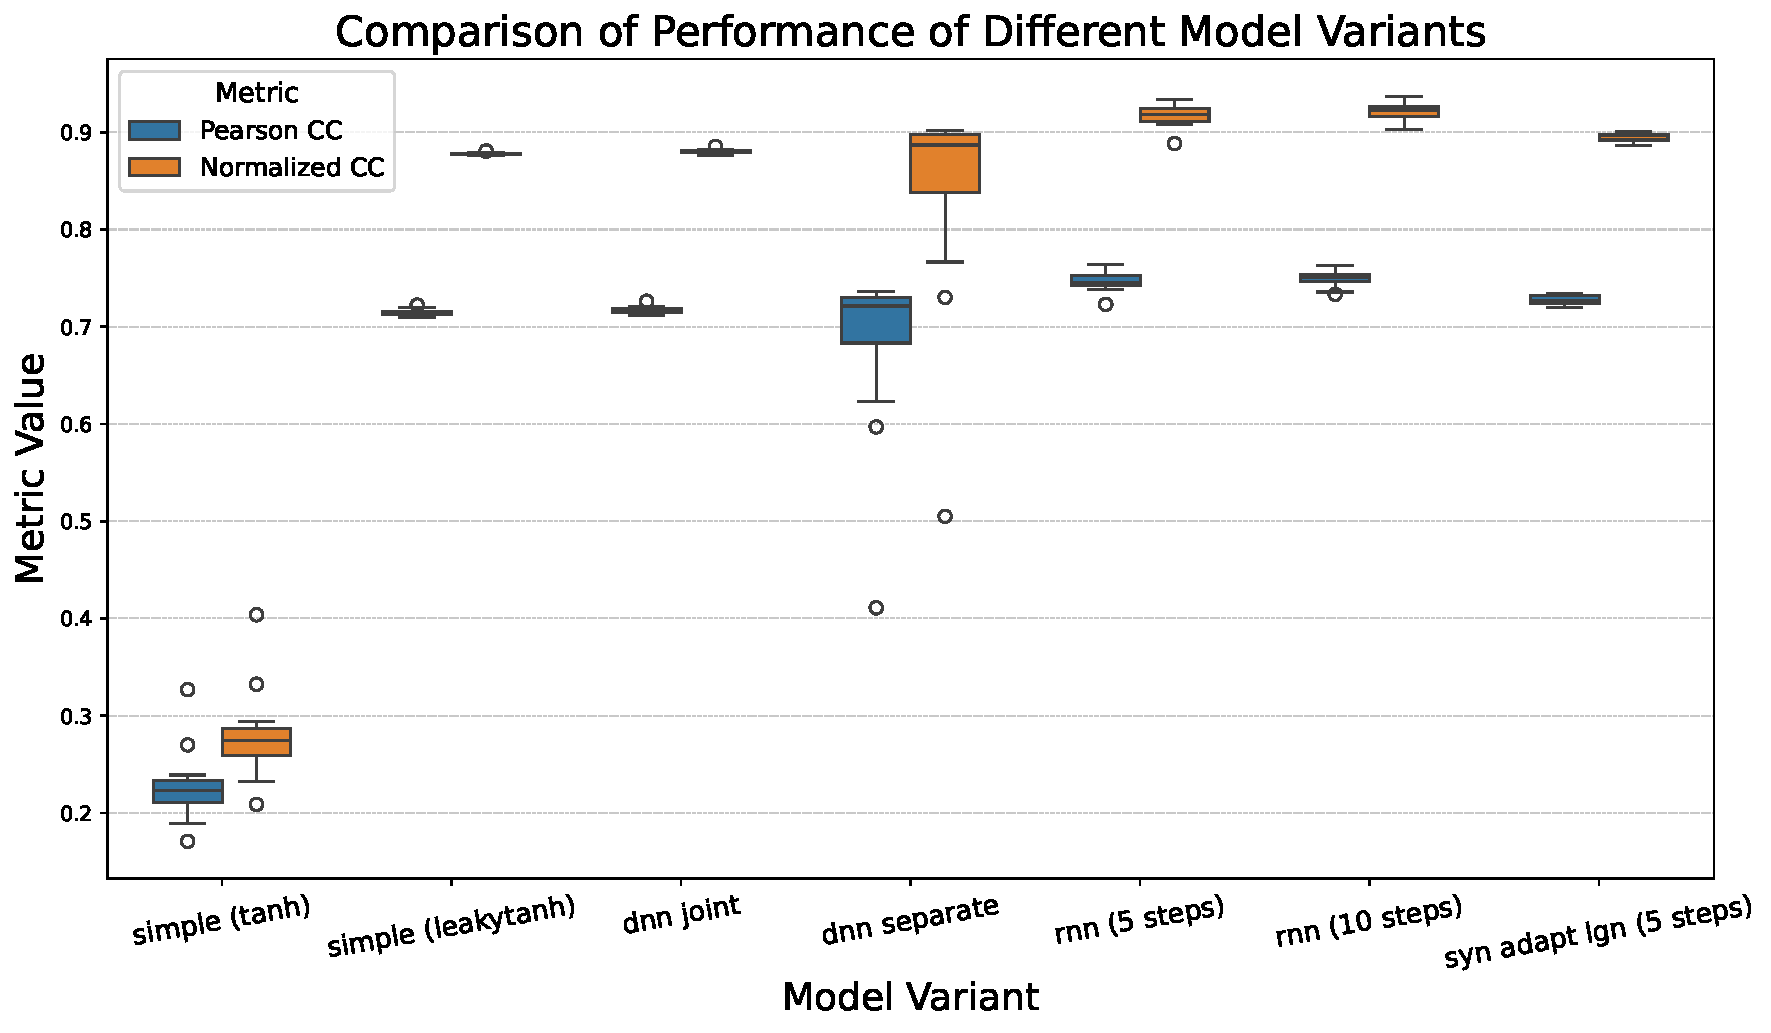
\includegraphics[width=\linewidth]{img/plots/model_types_correlation_comparison.pdf}
    \caption{Boxplot comparing mean Pearson correlation coefficients and normalized correlation coefficients of all model predictions between different model types across all model subsets.}
    \label{fig:model_types_correlation_comparison}
\end{figure}

Overall from the results we can clearly see that the pearson CC and Normalized CC behave fairly similar, only difference is the offset that is expected based on the definition of normalized CC that should be basically pearson CC normalized to smaller range. Building on that we assume from now on that these 2 metrics behave similarly on our data and we will use mainly normalized CC in the rest of our analyses if not stated differently.

From the results we can clearly see that there is one model outstander, the simple (tanh) that clearly performs the worst out of all tested models. On the other hand we can see that using the leakytanh activation function specially designed for the task performs surprisingly well even in the simple model and the model simple leakytanh is even comparable to dnn joint and dnn separate results. This may reflect the fact the the feed-forward dnn neuron modules represent some fairly simple function that we can approximate using some custom activation function like the leakytanh. However, we see that using rnn neuronal module improves our results which may indicate the importance of introducing the memory to our neurons and application of TBPTT training algorithm. 

Another possible explanation of the fact that simple model and feed-forward models performed fairly well is that they might capture the mean neuronal spiking pattern (as already mentioned in Section~\ref{subsec:deep_learning_approach}) and since the predicted neuronal responses are fairly sparse the high CC values might be caused due to the sparseness. On the other hand better results of TBPTT models might dawn of the temporal activity patterns in the predictions and thus sign of the model improvement.

Another interesting outstander is dnn separate model. This model performs strangely variable in comparison to other model variants. However, we do not really see the clear reason for this behavior. In fact this model should introduce the separation of the excitatory and inhibitory processing in the dnn modules and we expected that it would improve the predictions. Furthermore, while developing the model it showed fairly similar behavior to dnn joint model. For the rnn neuronal modules we have selected only the separate variants since the additional modules should sequentially add more biological plausibility and it really does not sense in our case to omit the layer separation. Also during our empirical tests this model performed fairly similar even sometimes better than the joint variants. We thus suggest that the strange variance might be cause by the not really representative number of results that contains only results for 20 model subset variants and that might be better captured by additional experimental runs on more model subsets. Additionally our testing dataset consists only of 20 trials that might not be enough to compute representative normalized CC values. For the future research it would be definitely worth it to run these experiments on the larger number of subset variants and with larger testing dataset including experiments and trials.

Overall of the models the best performing one seems to be rnn (10 steps) that shows reasonably variability across subset variants and performs best in terms of mean normalized CC. We might also suggest that adding more time steps to TBPTT calculation improves the results. However, experiments on larger number of time steps is not suitable for our experiments for time and memory consumption reasons and our restrained capability to access these.

The last interesting notice from the results is that it seems that the model syn adapt lgn (5 steps) performs worse than the models without synaptic depression module at all. We are not sure about the reason for this phenomenon but it might well be cause by the non-profound grid search for synaptic depression models as well with the necessity for usage of more TBPTT time steps and training epochs. These things unfortunately could not be tested due the computational demands of the synaptic depression models.

As the last part of the overview across all models we look at the correlation of the \emph{synchrony curves} for each model layer predictions. As it was already stated in Section~\ref{subsubsec:neuron_synchrony_binning} the synchrony of the time bin is a portion of the neurons in the layer that spike simultaneously at the given time step. The synchrony curve is then just temporal sequence of synchrony values across all time bins in the experiment. In the Figure~\ref{fig:boxplot_models_overall_synchrony_pearson_comparison} there is a boxplot comparing pearson CC of the model predictions (marked as overall CC) and of the synchrony curves (marked as synchrony CC) for all studied models. Note that there is a model simple (tanh) missing, because there has been technical difficulties during the evaluation and we were not able to replicate the results repeatedly for this model due to the time constraints. However, since we have already seen that this model does perform significantly worse than any other and our focus is mainly on the model of the highest level of biological relevance we claim that inclusion of only simple (leakytanh) give us enough insight into the simple model variant.

\begin{figure}
    \centering
    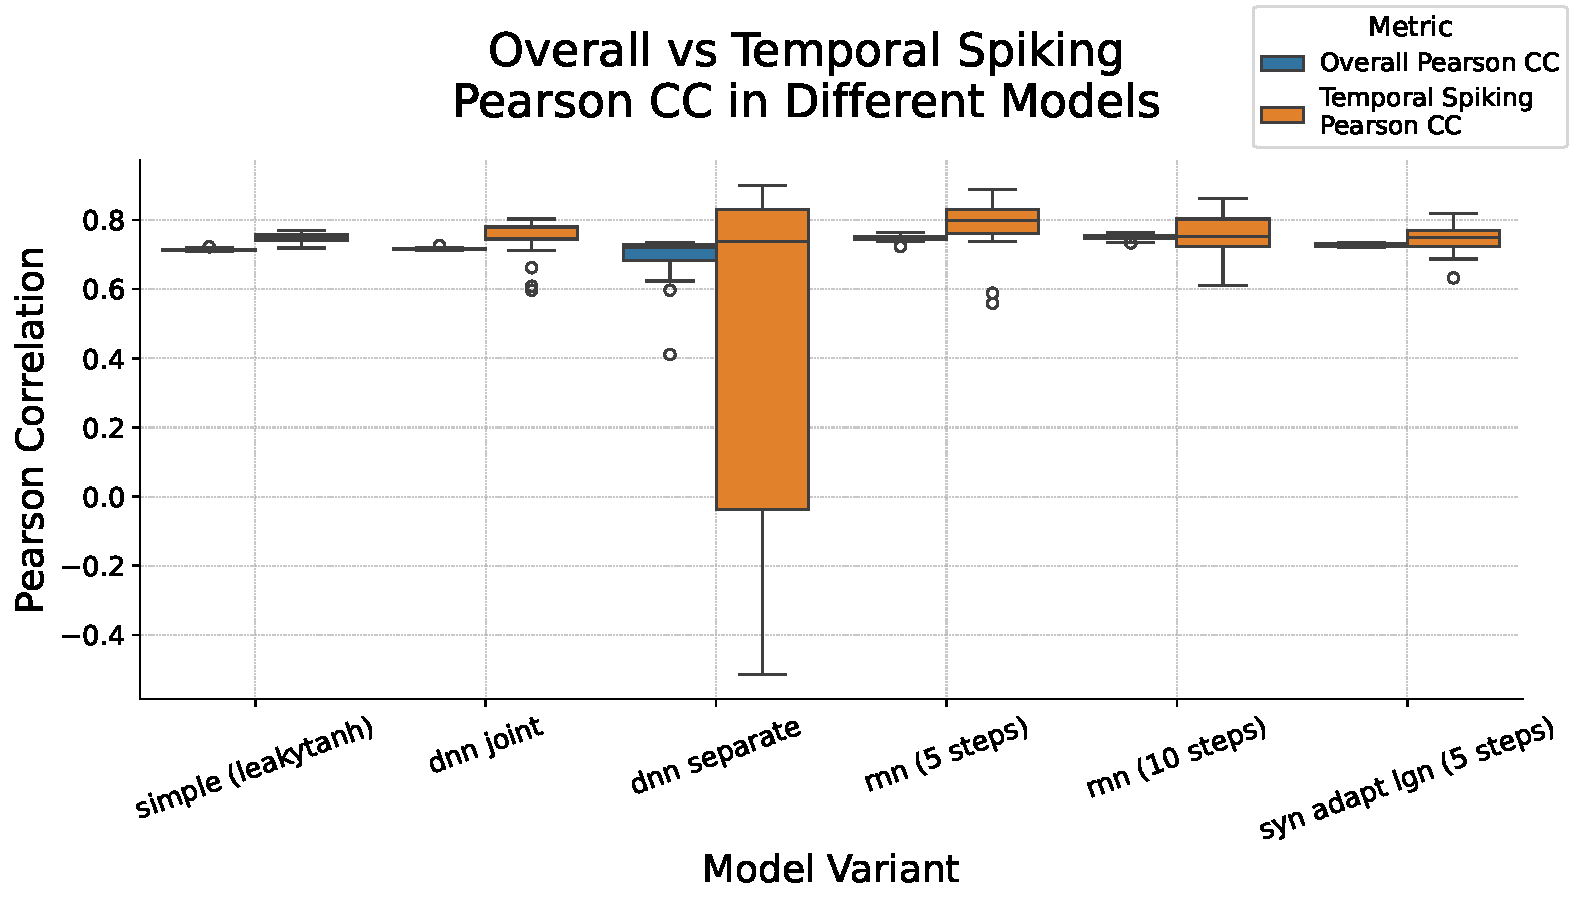
\includegraphics[width=\linewidth]{img/plots/boxplot_model_comparison_synchrony_overall_pearson.pdf}
    \caption{This figure shows comparison of distribution of pearson CC between model predictions and of model prediction synchrony curves across all layers and all model subset variants for each model type in respect targets.}
    \label{fig:boxplot_models_overall_synchrony_pearson_comparison}
\end{figure}

As we can see from the boxplot the variance of the synchrony CC is in all model types predictions higher than for overall CC. Another interesting fact is that models using TBPTT training algorithm are more variable in terms of the synchrony CC in comparison to other model except of the dnn separate that behaves strangely also in other metrics as already stated. This fact might be a sign of better captured dynamics of the model. In other words the fact that the temporal activity of the predictions vary more might be a sign that the model is trying to capture the temporal activity not just the mean of it through time. Additionally, it seems that synchrony CC and overall CC does not vary much in terms of mean and comparison between the models. One interesting fact is that in this metric the rnn (5 steps) behaves slightly better than rnn (10 steps) we do not really see the reason why this happened but since we see that there are more outliers of the model rnn (5 steps) synchrony CC, we might assume that this might be an effect of the small number of model variants that we have tested and in more robust experiment the results might differ.

As we have seen in the results previously the dnn separate model synchrony CC behaves strangely especially in its wide variance. This indicates some problematic model variants that is empowered by the occurrence of the low performing variants also in overall CC. Our hypothesis is that this is cause either by the selection of the subset variant that behaves badly only in dnn separate variance, or complexity of the input that is separated to excitatory and inhibitory and might be to complex for the small feed-forward network maybe because of the lack of some form of the memory. This statement supports the results of separate variants of rnn neuronal modules that behave the best across all tested variants. Last possible explanation that comes to our mind is the technical problem during the evaluation of some subset of the dnn separate models that we did not encounter and led to generally worse results in some subset variants.

\subsection{Prediction-Target Temporal Behavior of Model Variants}
\label{subsec:prediction_target_comparison_variants}
In this section we focus mainly on comparison of the temporal behavior of the model predictions separately. We will inspect how each model synchrony curves look like and compare them with the expected target synchrony curves. Note that we will not focus on the model simple (tanh) as there has been a technical difficulties during the evaluation part and we were not able to retrieve the model predictions and thus compute the synchrony curves. As already mentioned we do not expect this to be serious problem for our analysis as we already have in our analysis simple model variant included and the model with tanh activation behave generally the worst, so, we do not expect to obtain much insight from this model synchrony curves.

The idea behind the inspection of the synchrony curves is that these might unveil the temporal behavior of our model predictions that is the key aspect of the model that we want to capture correctly as this will be step forward in comparison to generally used approaches of NN models in system identification problem as mentioned in Section~\ref{subsec:deep_learning_approach}.

\subsubsection{Simple Model}
\label{{subsubsec:simpl_leakytanh_eval}}

First, we depict in the Figure~\ref{fig:synchrony_curve_simple_leaky_tanh} the synchrony curve of the simple (leakytanh) model predictions. 

\begin{figure}
    \centering
    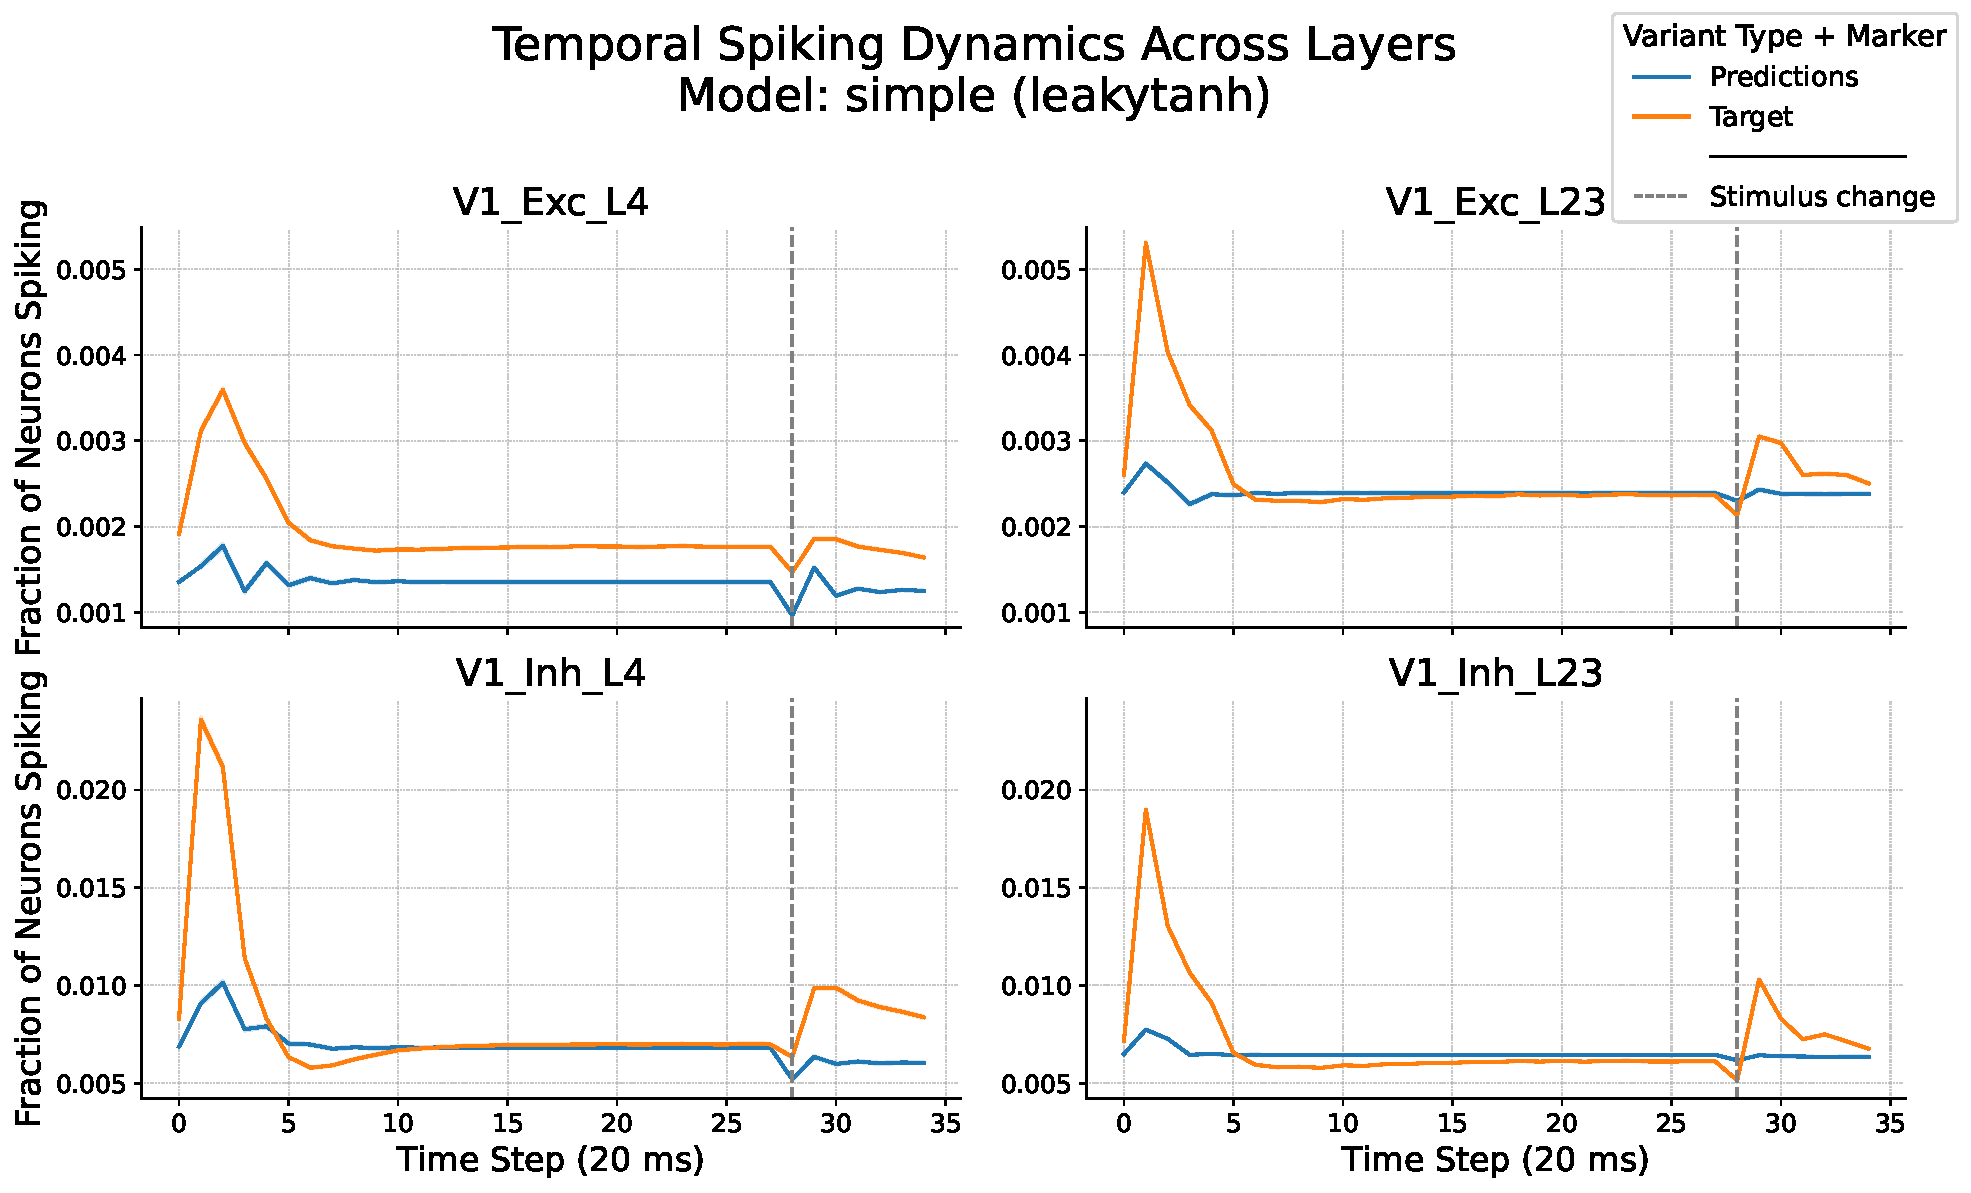
\includegraphics[width=\linewidth]{img/plots/separate_model_synchrony_curve_simple_evaluation_new.pdf}
    \caption{This figure depicts mean synchrony curve of simple (leakytanh) model predictions and its comparison to mean target synchrony curve both across all trials and all model subset variants including error bars. The dashed line marks the time step where the natural stimuli and blank stimuli changes.}
    \label{fig:synchrony_curve_simple_leaky_tanh}
\end{figure}

As we have already stated before it seems that the model mainly focuses on the prediction of the mean spiking rate across all time steps. We assume this by the flatness of the synchrony curve across the time that is the sign of not very dynamic activity. This leads to fairly reasonable results in the later stages of the stimuli part of the experiment but does not really capture the initial high spiking activity of the system in the early stage of the natural stimulus presentation. However this model surprisingly captures well the dynamics of the stimulus change when natural stimulus is replaced by the blank image. This as we will seen in the following models is captured fairly well also in comparison to other models. Lastly, as we can see that the model performs well mainly in the prediction of the mean spiking activity we might hypothesise that this is cause by the specially designed leakytanh activation function that focuses on the predictions in the reasonable interval of values and significantly enforce the model to predict values similar to mean neuronal responses. This influence of the leakytanh activation can be easily strenghten by the comparison to tanh variant that performed badly in terms of CC and eventhough we do not have the predictions of the neuronal responses for this model we assume that these will be much worse than currently tested simple (leakytanh) variant.

\subsubsection{Feed-Forward Neuronal Modules Variants}
\label{{subsubsec:dnn_eval}}
Now, we focus on the synchrony curves of models dnn joint in Figure~\ref{fig:synchrony_curve_dnn_joint} and dnn separate model in Figure~\ref{fig:synchrony_curve_dnn_separate}.
\begin{figure}
    \centering
    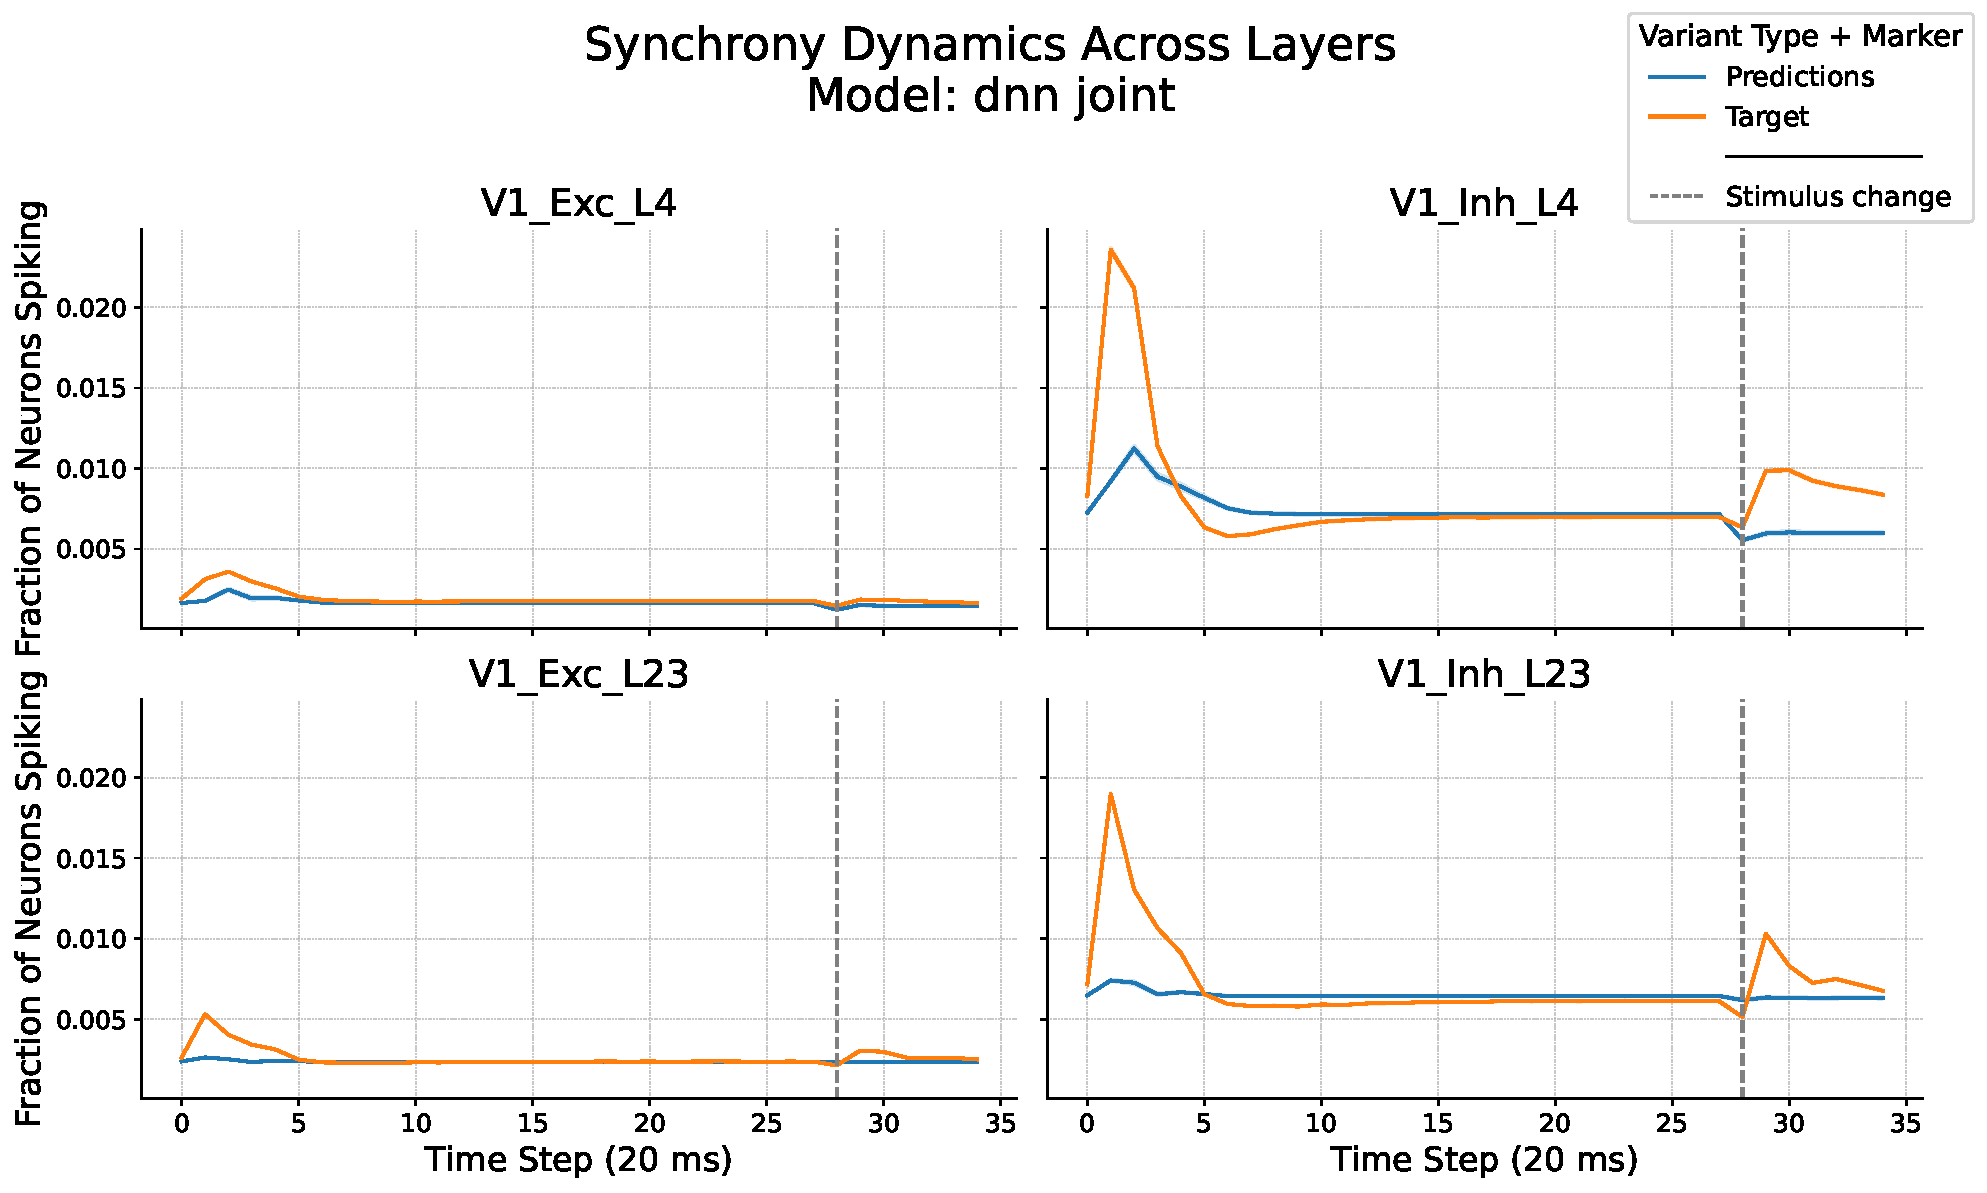
\includegraphics[width=\linewidth]{img/plots/separate_model_synchrony_curve_dnn_joint_evaluation.pdf}
    \caption{This figure depicts mean synchrony curve of dnn joint model predictions and its comparison to mean target synchrony curve both across all trials and all model subset variants including error bars. The dashed line marks the time step where the natural stimuli and blank stimuli changes.}
    \label{fig:synchrony_curve_dnn_joint}
\end{figure}

\begin{figure}
    \centering
    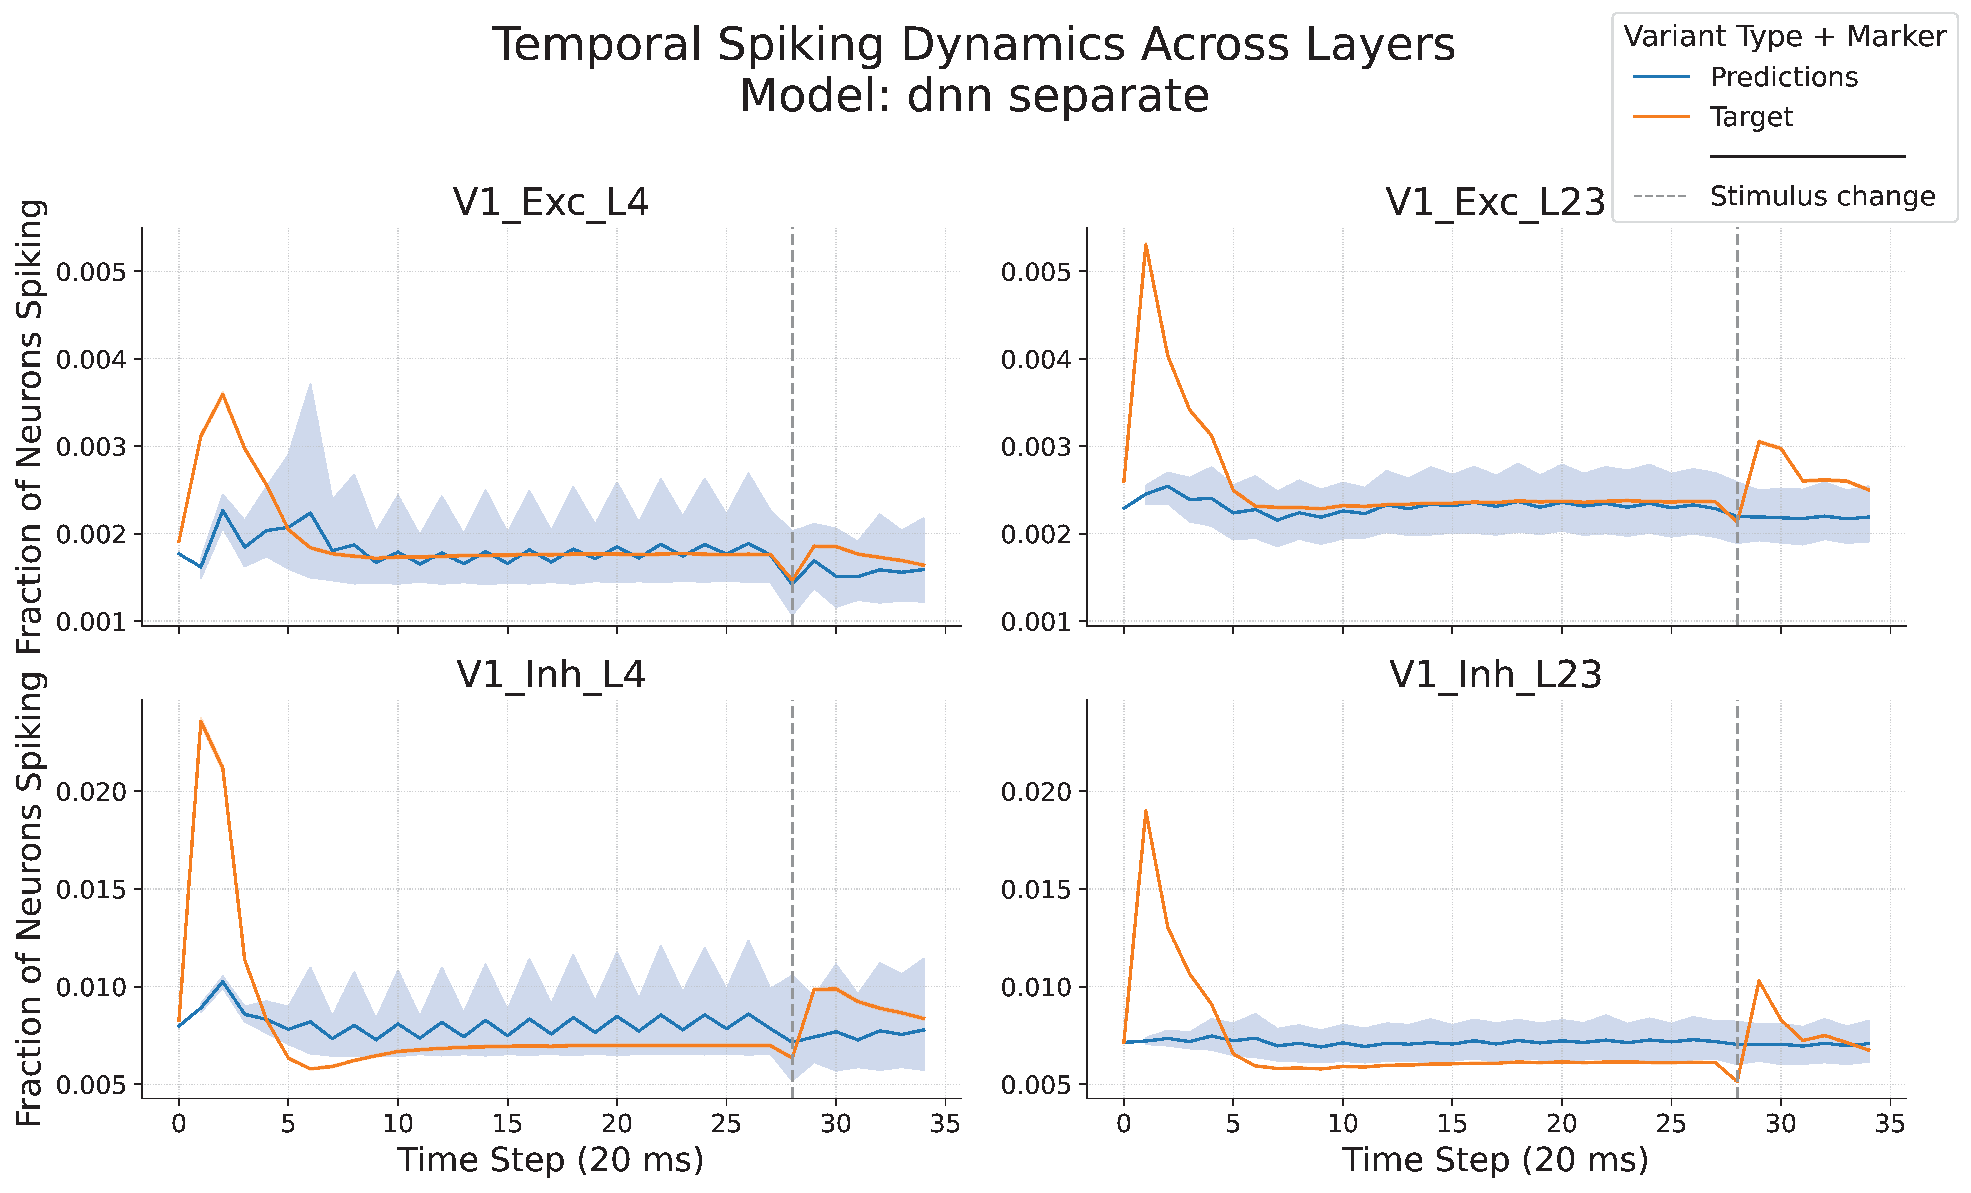
\includegraphics[width=\linewidth]{img/plots/separate_model_synchrony_curve_dnn_separate_evaluation.pdf}
    \caption{This figure depicts mean synchrony curve of dnn separate model predictions and its comparison to mean target synchrony curve both across all trials and all model subset variants including error bars. The dashed line marks the time step where the natural stimuli and blank stimuli changes.}
    \label{fig:synchrony_curve_dnn_separate}
\end{figure}

As we have already stated the model dnn separate behaves strangely noisy that can be also seen mainly in the error bars of its synchrony. As we have already discussed the causes of this phenomenon we will not focus on this model anymore. 

In terms of the dnn joint model we do not really see significant difference in comparison to simple (leakytanh). There is a sign of the better initial activity as a response to early natural stimuli stages. Overall, these might be a sign that feed-forward neuron modules improved the temporal behavior a bit but as we can see the model still mainly captures the mean spiking behavior. Based on these fact we conclude that the as we used simple feed-forward NN we can capture only slightly more complex activation function than is leakytanh that leads to slightly better temporal behavior. However, since these modules do not have any form of "memory" and information about the past stimuli they are not really sufficient in the capturing of the temporal behavior. 

\subsubsection{RNN Neuronal Modules Variants}
\label{{subsubsec:rnn_eval}}
The findings of the already tested variants naturally leads us to the usage of RNN model variants that use TBPTT time training algorithm that allows the model better see the temporal behavior of the network during the training and thus may lead to better predictions of the temporal behavior. Although the already tested variants have recurrent connections that capture the biological realism and that allows the temporal self-modulation we do not really allow the training algorithm to compute gradients over time since we reset the hidden states after each time step by the target neuronal responses. This is often called \emph{teacher-forced} training (\citet{NIPS2016_16026d60}). The network then theoretically can capture the temporal dynamics but since we do not use any hidden time steps we constraint our model from backpropagation through time training algorithm and be introducing the temporal behavior during training. In the following models this is however included.

As we can see from the Figure~\ref{fig:synchrony_curve_rnn_5} and Figure~\ref{fig:synchrony_curve_rnn_10} that depicts the synchrony curves of the rnn separate model using TBPTT training algorithm for either 5 respectively 10 time steps the overall temporal behavior improved without doubt. We can see that there is a massive improvement in the prediction of the early stages of the natural stimuli that nicely captures the overall dynamics. The only flaws of the predicted dynamics that still persist are the neuronal responses to blank stimuli that in our model predictions does not really differ from later responses on natural stimuli but in target responses the spiking activity to blank stimuli also called as spontaneous neuronal activity (briefly mentioned in Section~\ref{subsec:stimulus_sequence}) is higher than later natural stimuli stages indicating the suppressed neuronal activity to the long term presented stimulus.

\begin{figure}
    \centering
    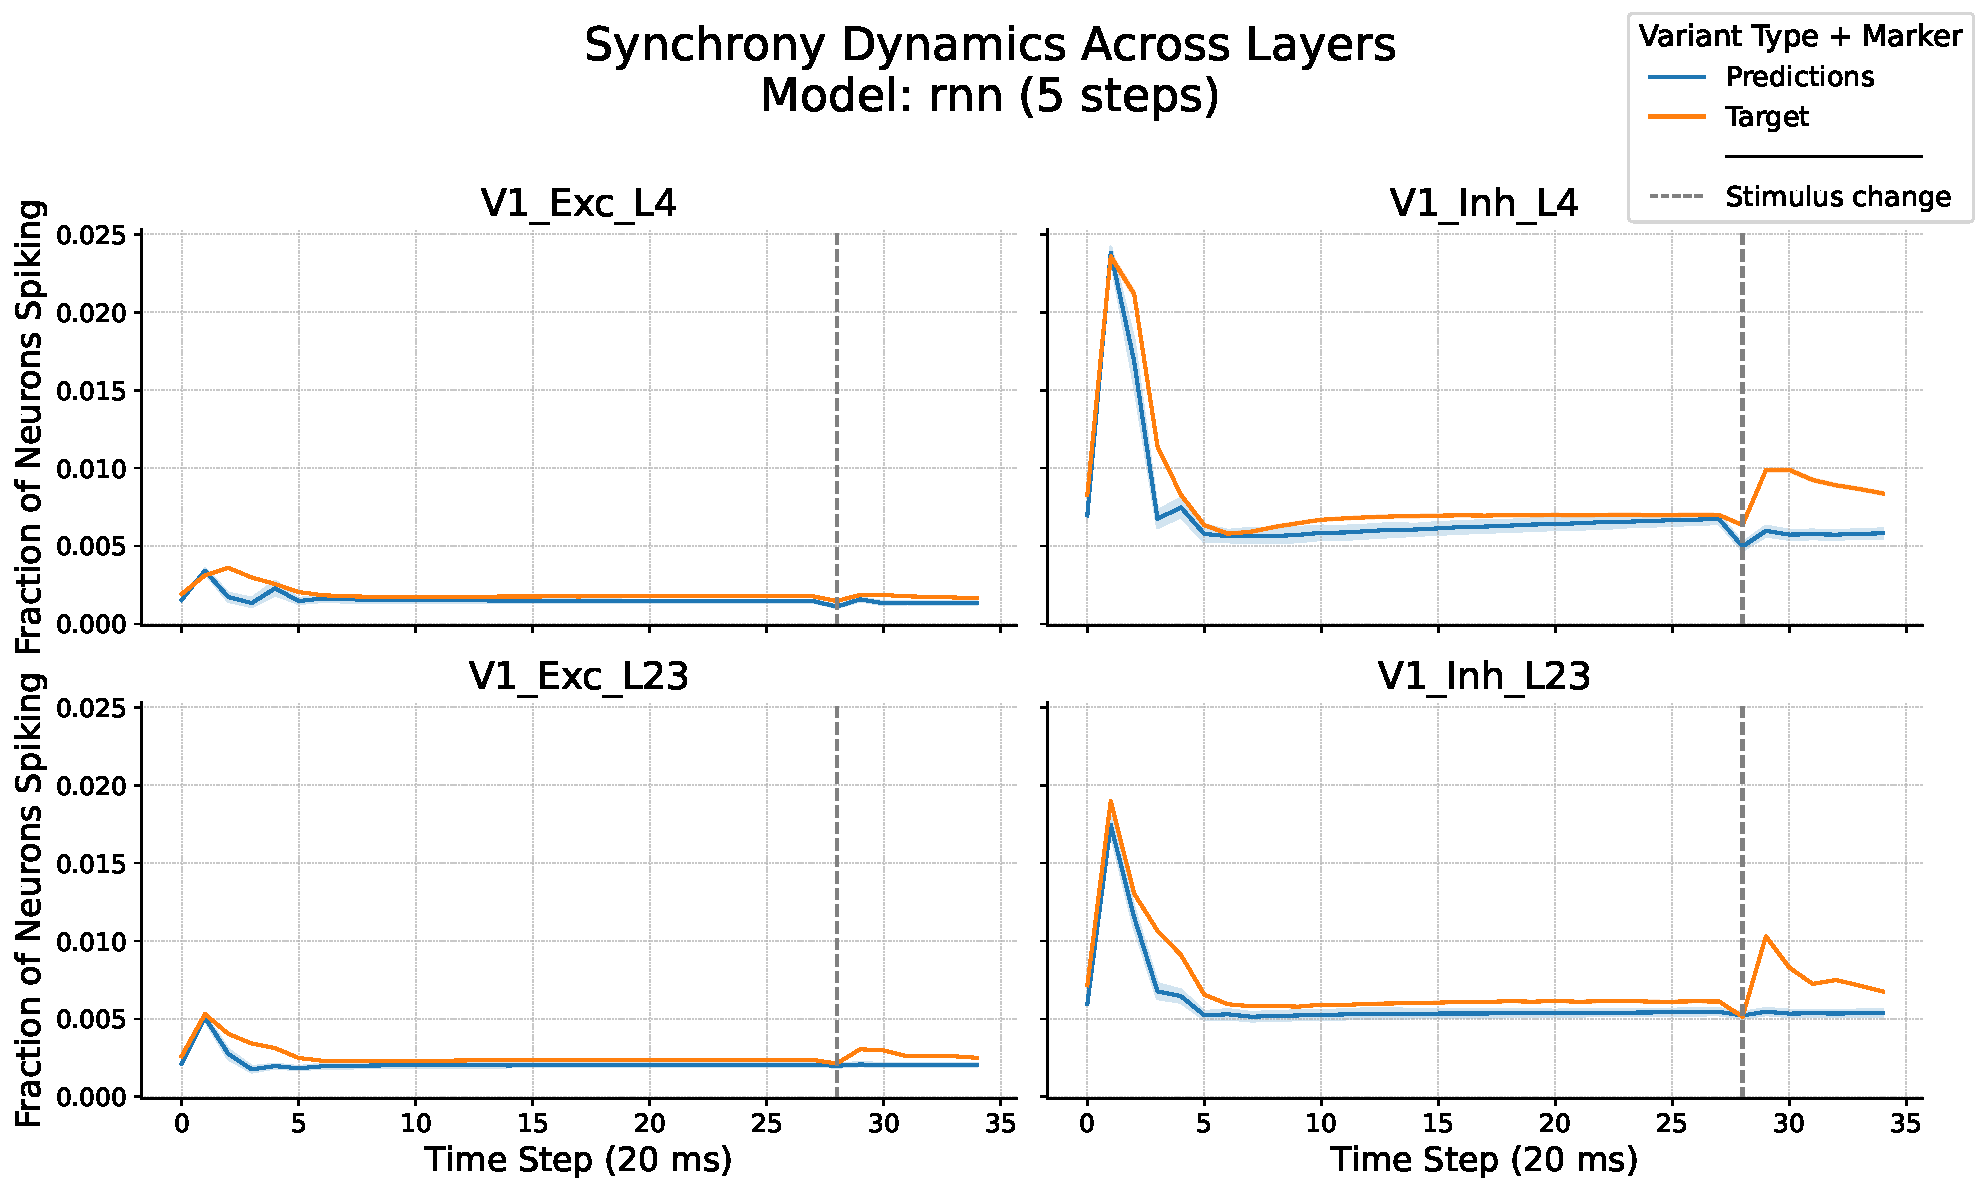
\includegraphics[width=\linewidth]{img/plots/separate_model_synchrony_curve_rnn_separate_5_evaluation.pdf}
    \caption{This figure depicts mean synchrony curve of rnn (time 5) model predictions and its comparison to mean target synchrony curve both across all trials and all model subset variants including error bars. The dashed line marks the time step where the natural stimuli and blank stimuli changes.}
    \label{fig:synchrony_curve_rnn_5}
\end{figure}

\begin{figure}
    \centering
    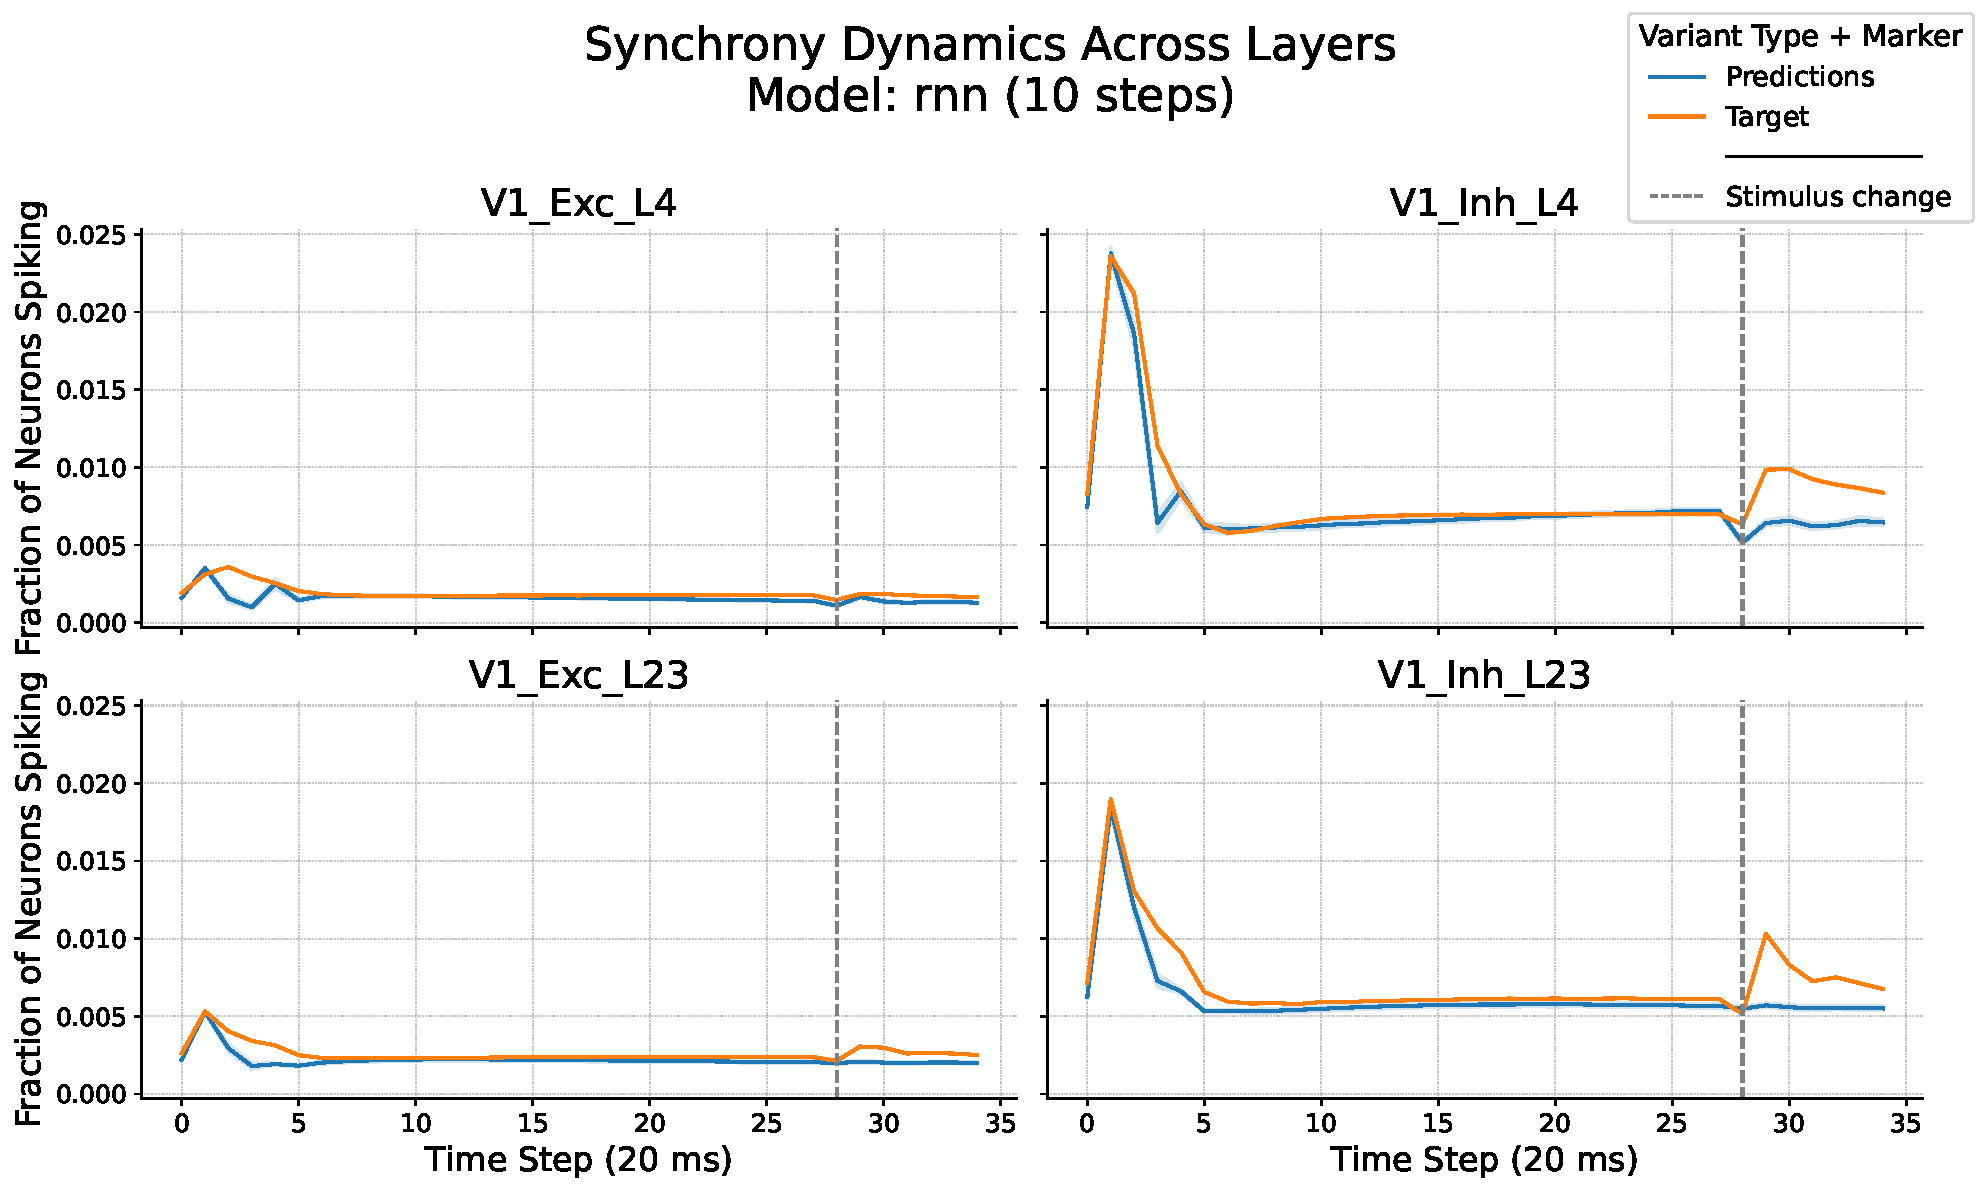
\includegraphics[width=\linewidth]{img/plots/separate_model_synchrony_curve_rnn_separate_10_evaluation.pdf}
    \caption{This figure depicts mean synchrony curve of rnn (time 10) model predictions and its comparison to mean target synchrony curve both across all trials and all model subset variants including error bars. The dashed line marks the time step where the natural stimuli and blank stimuli changes.}
    \label{fig:synchrony_curve_rnn_10}
\end{figure}

While comparing the models using either 5 or 10 TBPTT time steps we conclude that higher number of time steps improve the model performance as from the synchrony curves it seems that the dynamics is better in the predictions of the model rnn (10 steps) also in terms of noisiness across the subset variants. This claim is empower by the findings that the rnn (10 steps) performed in fact the best of tested model variants in terms of both normalized and pearson CC.

Looking on the synchrony curve we can now briefly reflect again on the synchrony pearson CC displayed in Figure~\ref{fig:boxplot_models_overall_synchrony_pearson_comparison} where we see that the synchrony CC is strangely more variable in the TBPTT models in comparison to the rest of the models. As we look at the synchrony curves we assume that this fact may be indeed caused by the higher and better dynamics of the TBPTT models. Furthermore, the seemingly comparable CC mainly in terms of synchrony CC is probably caused by the preference of non TBPTT models to capture the mean responses in comparison to more dynamic TBPTT models. The better capture of the quite stable later natural stimulus stage in the non TBPTT models probably leads to high values of the CC. On the other hand since the TBPTT models are more dynamic then nicely capture the response dynamics but is not that precise in non-dynamic behavior.

The fact that rnn neuron model variants capture the dynamics better is a good sign towards the development of deep neural network model that is biologically explainable and that captures the dynamics reasonably well (as mentioned profoundly in Section~\ref{subsec:deep_learning_approach} and Section~\ref{subsec:spiking_neural_nets}).

\subsubsection{Synpatic Depression Model}
\label{{subsubsec:syn_adap_lgn_5}}
In the last part of the analysis of synchrony curves we focus on the usage of the synaptic depression module. As mentioned in the previous section there are still flaws in the temporal dynamics of the spontaneous neuronal responses during the blank stage. This naturally leads to inclusion of the synaptic depression modules different for each pair of the layers. This should include the separation of the dynamical adaptation to the neuronal activity from the different neuronal populations and thus to improvement of the temporal behavior.

We have performed the experiments including neuronal depression only on the model variant using 5 TBPTT time steps and only including the neuronal depression module on the LGN connections as these are the ones that in the biological network are most influenced by this phenomenon. The synchrony curve of the model predictions is depicted in the Figure~\ref{fig:synchrony_curve_syn_adapt_lgn_5}. 

\begin{figure}
    \centering
    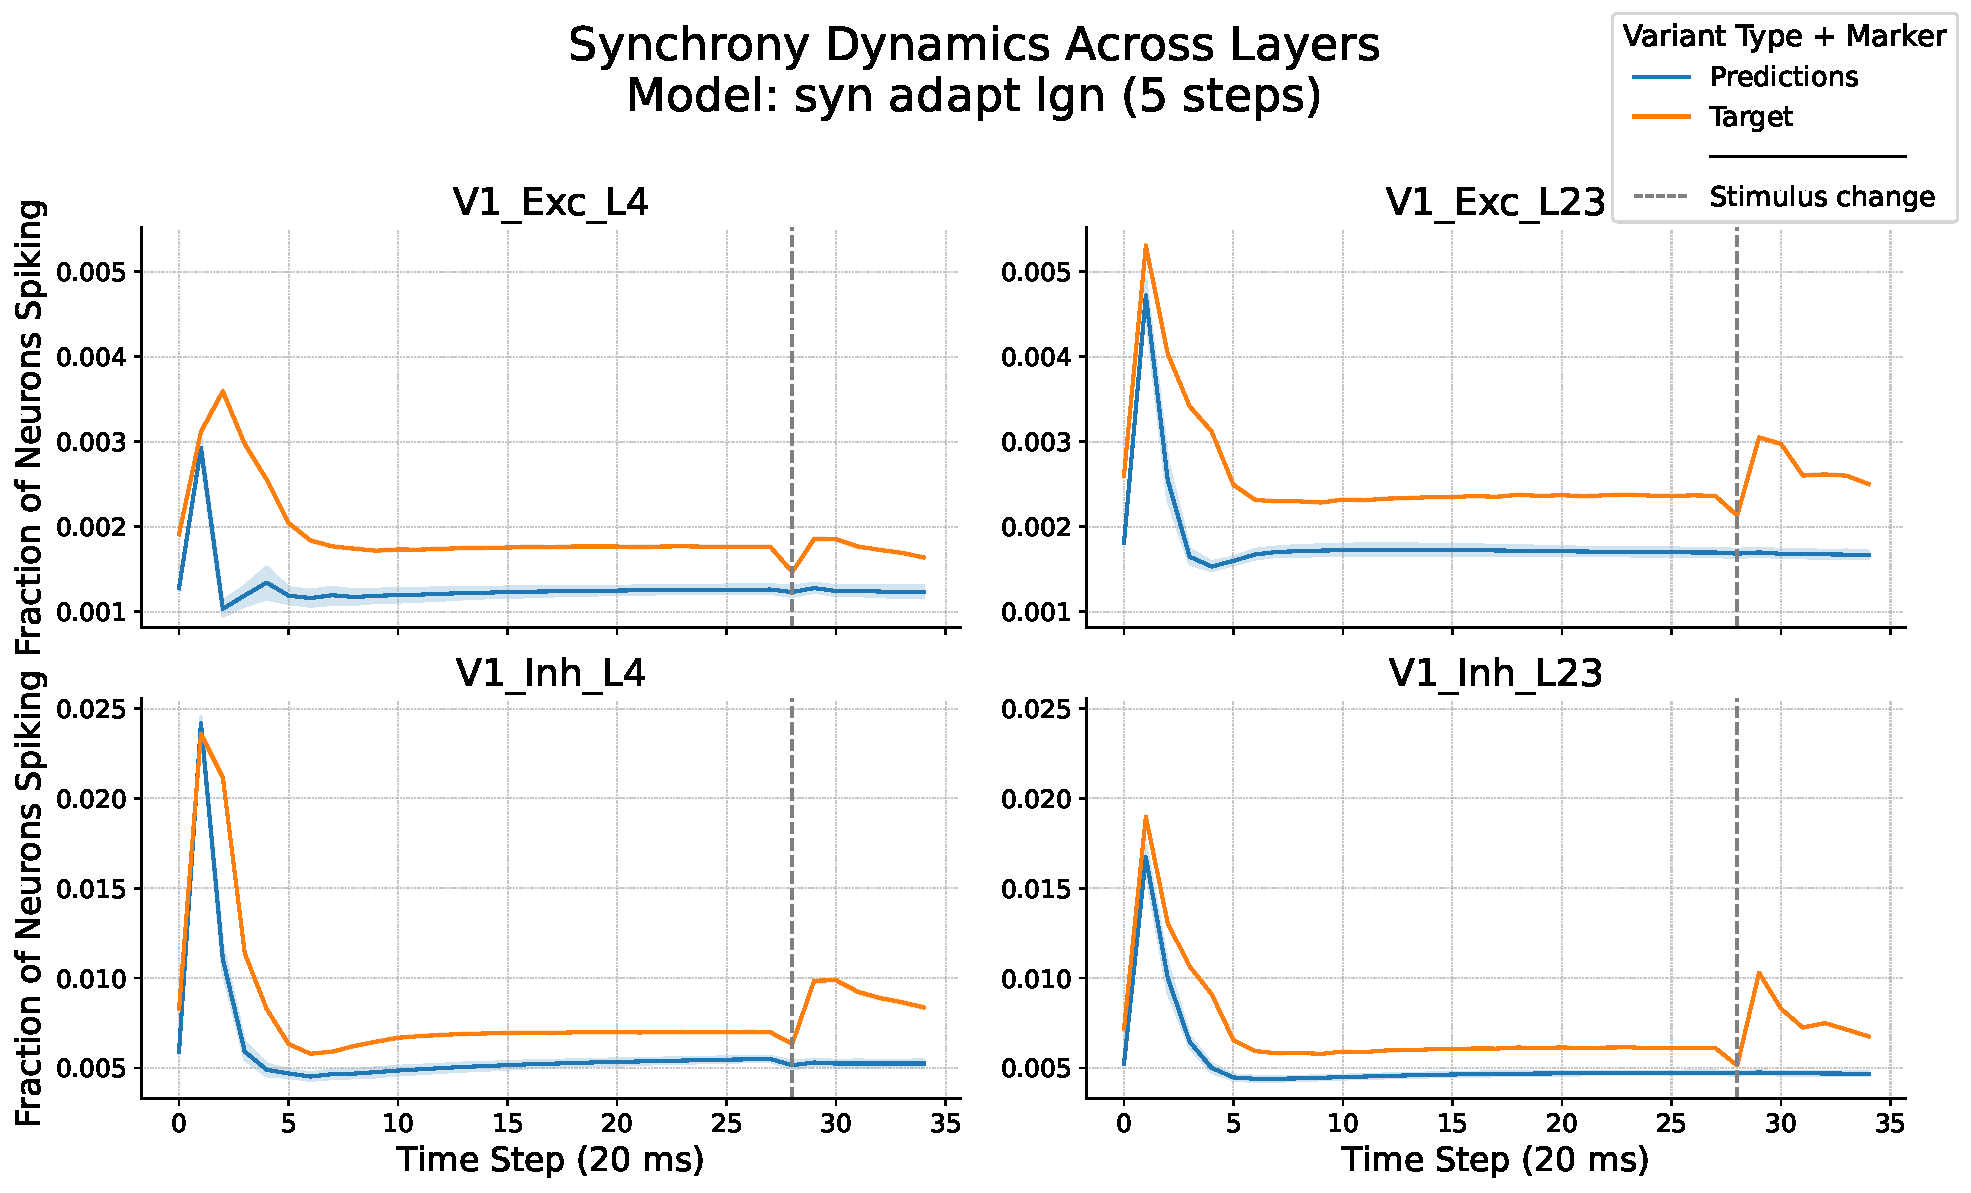
\includegraphics[width=\linewidth]{img/plots/separate_model_synchrony_curve_syn_only_lgn_5_evaluation.pdf}
    \caption{This figure depicts mean synchrony curve of syn adapt lgn (time 5) model predictions and its comparison to mean target synchrony curve both across all trials and all model subset variants including error bars. The dashed line marks the time step where the natural stimuli and blank stimuli changes.}
    \label{fig:synchrony_curve_syn_adapt_lgn_5}
\end{figure}

The mentioned simplification has been done due several technical difficulties that we have encountered. The difficulties are mainly related to the largely rising necessity for the high memory GPU machines since each RNN synaptic depression module largely increase the memory consumption with increasing TBPTT time steps. Additionally, inclusion of these significantly prolongs the computational time of the model training. As a result of these problems we also have not been able to perform profound grid search for selection of the ideal hyperparameter and we have been forced to select the hyperparameters without that deep knowledge that we had for other model variants. These difficulties might lead to not really representative results of the model performance and might explain several non-clarities regarding this model performance.

As we can see from the synchrony curve the temporal behavior is definitely better that in terms of non TBPTT model, however, worse than in terms of rnn models without synaptic depression module. Interestingly, the model predictions seemingly worsen across all time interval. We can see significantly worsen performance in terms on dynamics at the change from natural stimuli to blank stimuli and also in terms of mean responses (the later natural stimuli stages). Furthermore, the performance neither improve in spontaneous responses (blank stage). 

These findings are surprising as we have expected the improved performance of the model while including more of the biological realism. Only explanation of this that comes to our mind is the non-ideal selection of the hyperparameters. Additionally, the problem might be related to small number of TBPTT time steps and lack of variable training dataset that might cover the dynamics of the network better.

\subsection{Model Performance Statistical Comparison}
\label{subsec:model_performance_statistical_comparison}

To empower our claims about the various model performance we have decided to conduct pairwise one-sided Mann-Whitney U test (\citet{mann_whithey_1947}) to test whether the distribution of normalized CC from one model are greater or equal to the normalized CC of the other model. We have selected this test because we do not know from which distribution our sampled normalized CC come from, so, we cannot really use some stronger more powerful parametric test. This test tests hypothesis that the two sampled groups are taken from the same distribution. Since we are using the one-sided variant we test the hypothesis that one sample is sampled from the distribution that is greater or equal to the other population. We have visualized the p-values of each tested pair in the heatmap depicted in the Figure~\ref{fig:model_types_p_values_heatmap}. In this heatmap the model in the row symbolizes the model that performs better in terms of the normalized CC in comparison to model in the row.

\begin{figure}
    \centering
    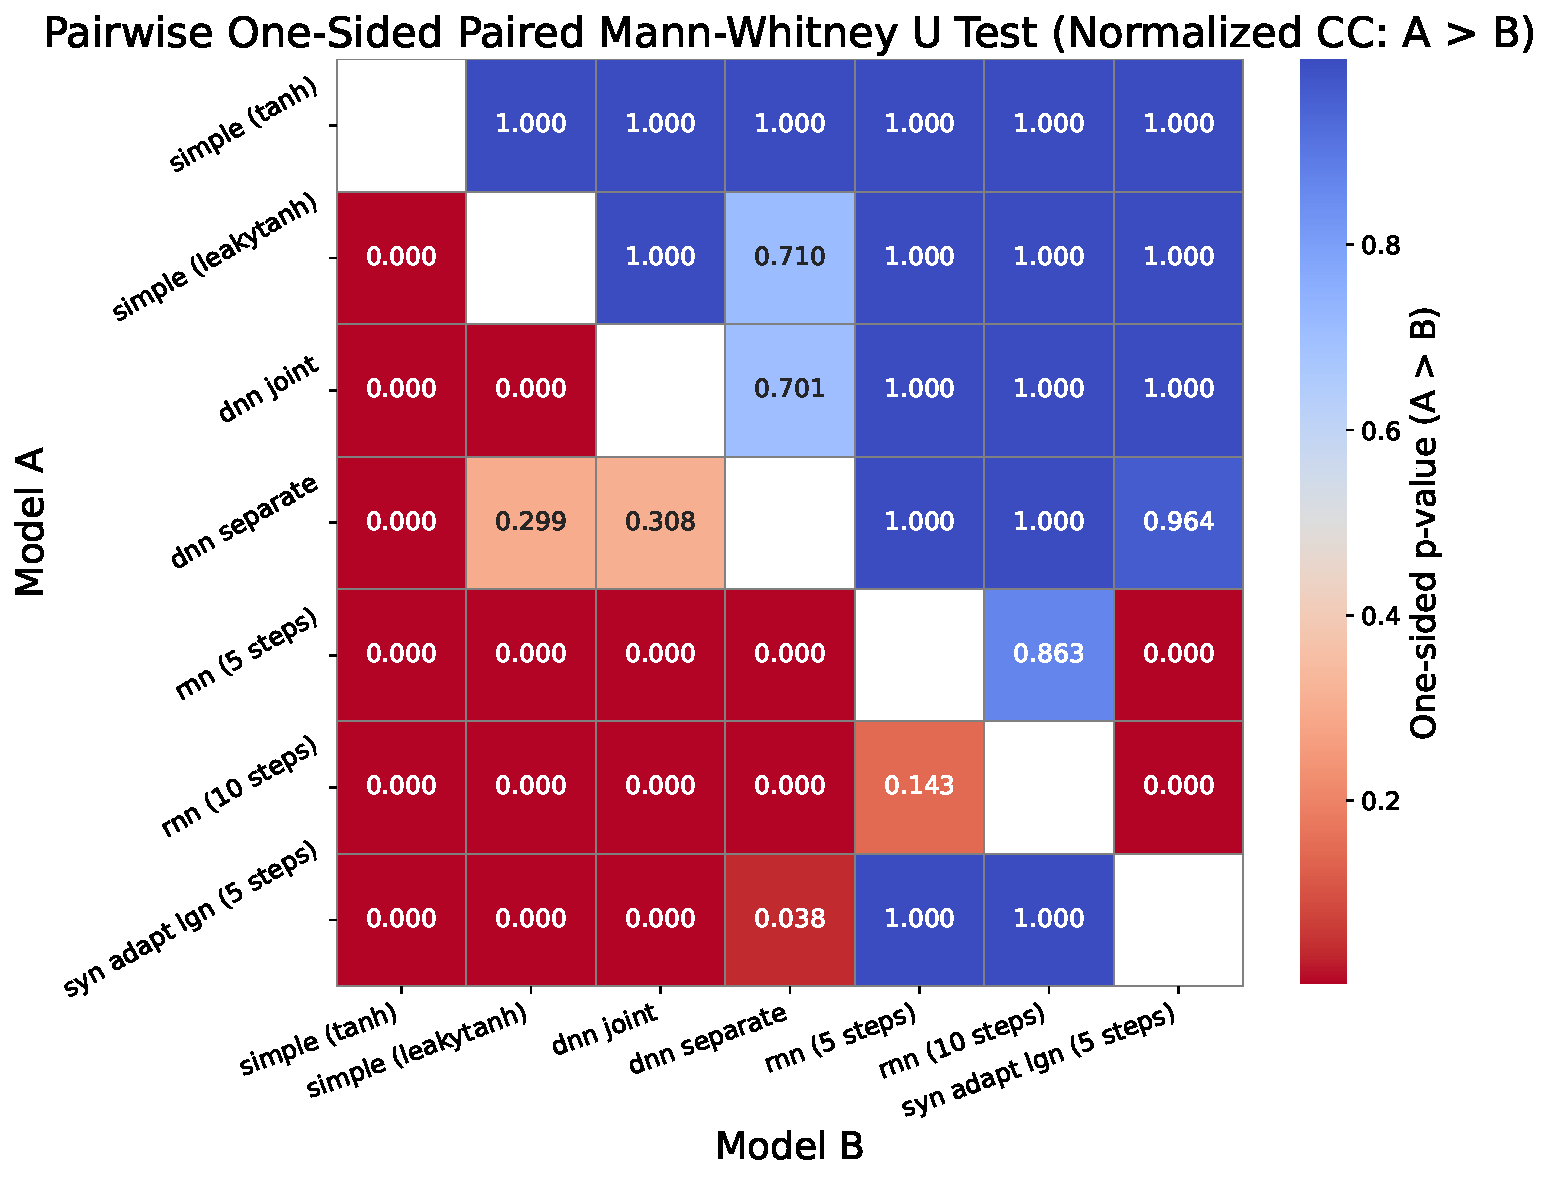
\includegraphics[width=\linewidth]{img/plots/model_types_p_value_heatmap_cc_norm.pdf}
    \caption{Heatmap that shows the p-value of pairwise one-sided Mann-Whitney U test. The test has been performed on the values of normalized cross correlation of each subset of each model variant. The test should say whether one of the model has significantly higher normalized cross correlation values. In each tile the row value marked as "Model A" represents the model that is tested to perform better and column value marked as "Model B" represents the model that is tested to perform worse. Assuming significance level $\alpha=0.05$ the value smaller than $\alpha$ decline the null hypothesis that the normalized cross correlation distribution is the same or worse for "Model A".}
    \label{fig:model_types_p_values_heatmap}
\end{figure}

The tests mainly confirms our claims that we have concluded from the box plots and the mean and standard deviation. If we assume the significance level $\alpha=0.05$ then we decline the hypotheses that simple (tanh) performs better than arbitrary other model variant. While looking at the other variants it mostly seems that the more complex models perform better with two exceptions. The dnn separate model that behaved strangely mainly in terms of the large variance that we already mentioned and the syn adapt lgn (5 steps) that interestingly seems to perform worse than the rnn model variants without the synaptic depression modules. This fact may be caused by the several constraints already mentioned before connected to constrained computational resources and thus not that profound analysis of the hyperparameters. Additionally, we have not tested the synaptic depression variant that applies the synaptic depression module to all connections since its computational complexity.

Overall, based on the high level metrics of person CC and normalized CC we assume that majority of our additional modules improved our model performance and that additional biological constraints might lead to improved modeling of the neural responses. The only two exceptions that seemingly contradicts this statement are dnn separate model and syn adapt lgn (step 5) model. These facts we mainly assign to our limited ability to test the model performances deeply and thus our results might not cover all model properties comprehensively as already stated before.

\section{Performance Gaps and Opportunities for Improvement}
\label{sec:performace_gaps_and_opportunities_for_improvement}
Until now, we have compared the different model approaches. With exception of the synaptic depression module we have concluded that increase biological realism improve the model performance. However, we have still seen some flaws in the model predictions especially in the temporal behavior of the spontaneous neuronal responses. In this section we will focus on several aspects of the model and we will try to figure out possible source of the model performance issues.
\subsection{Free vs Teacher-Forced Prediction Analysis}
\label{{subsec:free_vs_teacher_forced_predictions}}
First, we will focus on the comparison of the model performance while applying teacher-forced evaluation, the one that resets hidden states after each time step prediction with the appropriate target values, and the free prediction, the classical RNN prediction of the sequence of neuronal responses. We will focus mainly on the best performing model variants using TBPTT and that seems to be the right approach towards the better model performance as well as towards the biological relevance. 

Although, we first look at the boxplots of the synchrony CC of both teacher-forced and free predictions across all tested models without simple (tanh) per layer that is depicted in the Figure~\ref{fig:boxplot_models_pearson_synchrony_different_layers}.

\begin{figure}
    \centering
    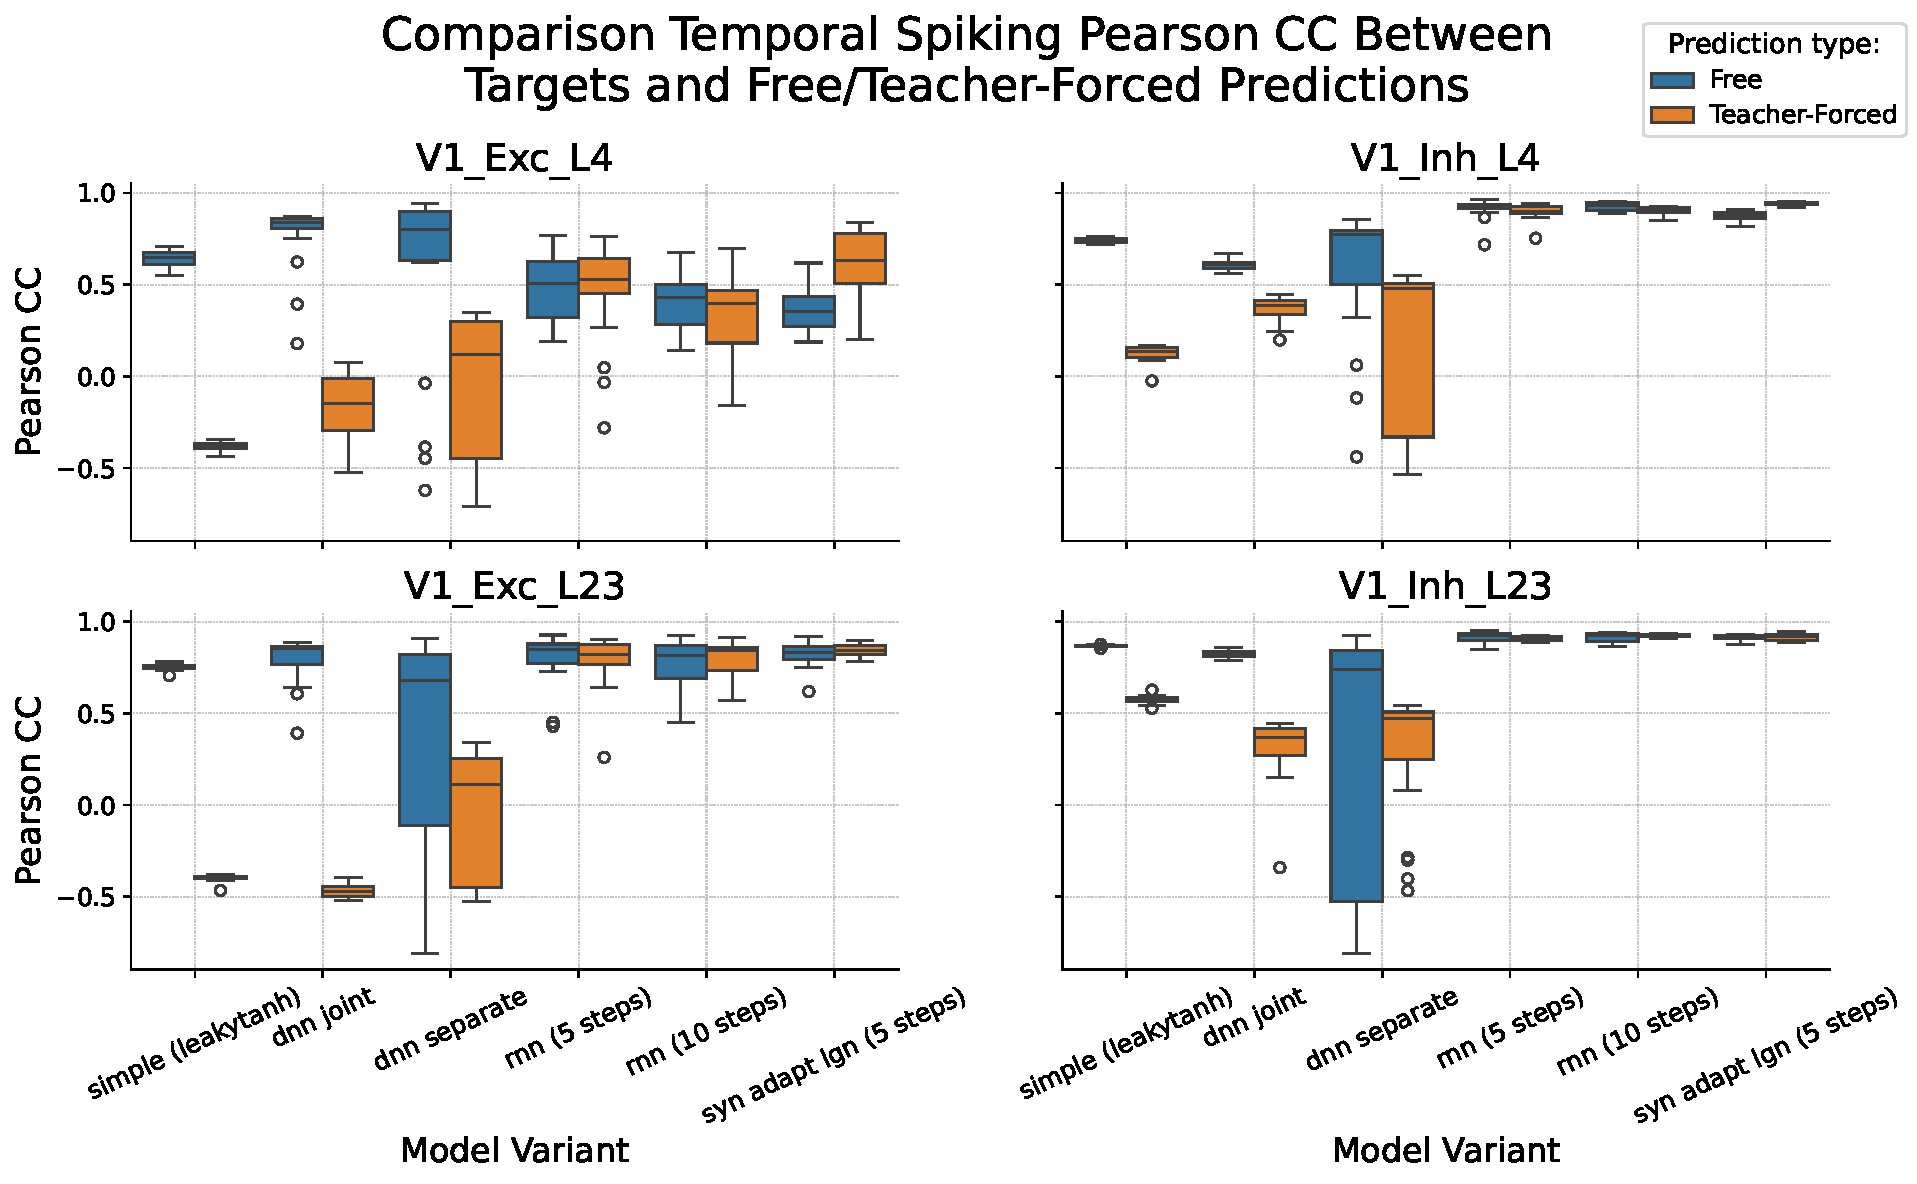
\includegraphics[width=\linewidth]{img/plots/boxplot_model_comparison_synchrony_pearson_layers.pdf}
    \caption{This figure shows comparison of distribution of pearson CC between model prediction and target synchrony curves separately for each layer.}
    \label{fig:boxplot_models_pearson_synchrony_different_layers}
\end{figure}

As we have seen many times the model dnn separate behaves strangely. Interestingly though the CC performance differ quite a lot across layer types. Overall, the CC of the TBPTT models seems to be the best across all layers. The more problematic layers seems to be the excitatory ones for these models also in comparison to the non TBPTT models. We hypothesize that this fact may be a cause of the relatively sparse activity of the excitatory layers as we have seen in the synchrony curves. The neurons in these layers generally do not spike that much and the fact the non TBPTT models capture the mean dynamics pretty well may also lead to better performance of these variants in the excitatory layers. On the other hand, we can see that in the more active inhibitory layers the TBPTT model variants performs the best. 

Interestingly, the teacher-forced predictions seems to be comparable and sometimes better in the TBPTT models. This is not that surprising since we expect that our models should capture the temporal dynamics reasonably well and thus reset of the hidden states should not cause significant difference in the model predictions since we expect our models would predict those reasonably well, so, the reset of state may just a bit tweak our model towards better predictions since the input hidden state is more appropriate for the next sequence step. 

As we can see the model performance improved the most while using teacher-forced variant in the synaptic depression model. This might be a sign that this model does not really learn the dynamics correctly and maybe additionally time steps in TBPTT or longer training might improve our model performance. 

Lastly, interesting fact is that non TBPTT performed worse while using teacher-forced variant. One might expect that since the models does not really seen the temporal sequence during the training that hidden state reset might improve the model temporal performance since this approach mimics the training stages. Our claim on this is that since the models capture mainly the mean responses the reset of states mainly in the initial stages of the experiment sequence where there is a hight spiking activity distracts the model predictions from the correct mean predictions and as a result worsen the overall model score.

\subsubsection{Teacher-Forced Synchrony Curves on TBPTT Model Variants}
\label{subsubsec:teacher_forced_synchrony_curves_tbptt}
From now on, let us focus only on TBPTT model variants. First we plot the synchrony curves for all the models for both free and teacher-forced predictions in comparison to targets. This is depicted in the Figure~\ref{fig:free_vs_teacher_forced_synchrony}.

\begin{figure}
    \centering
    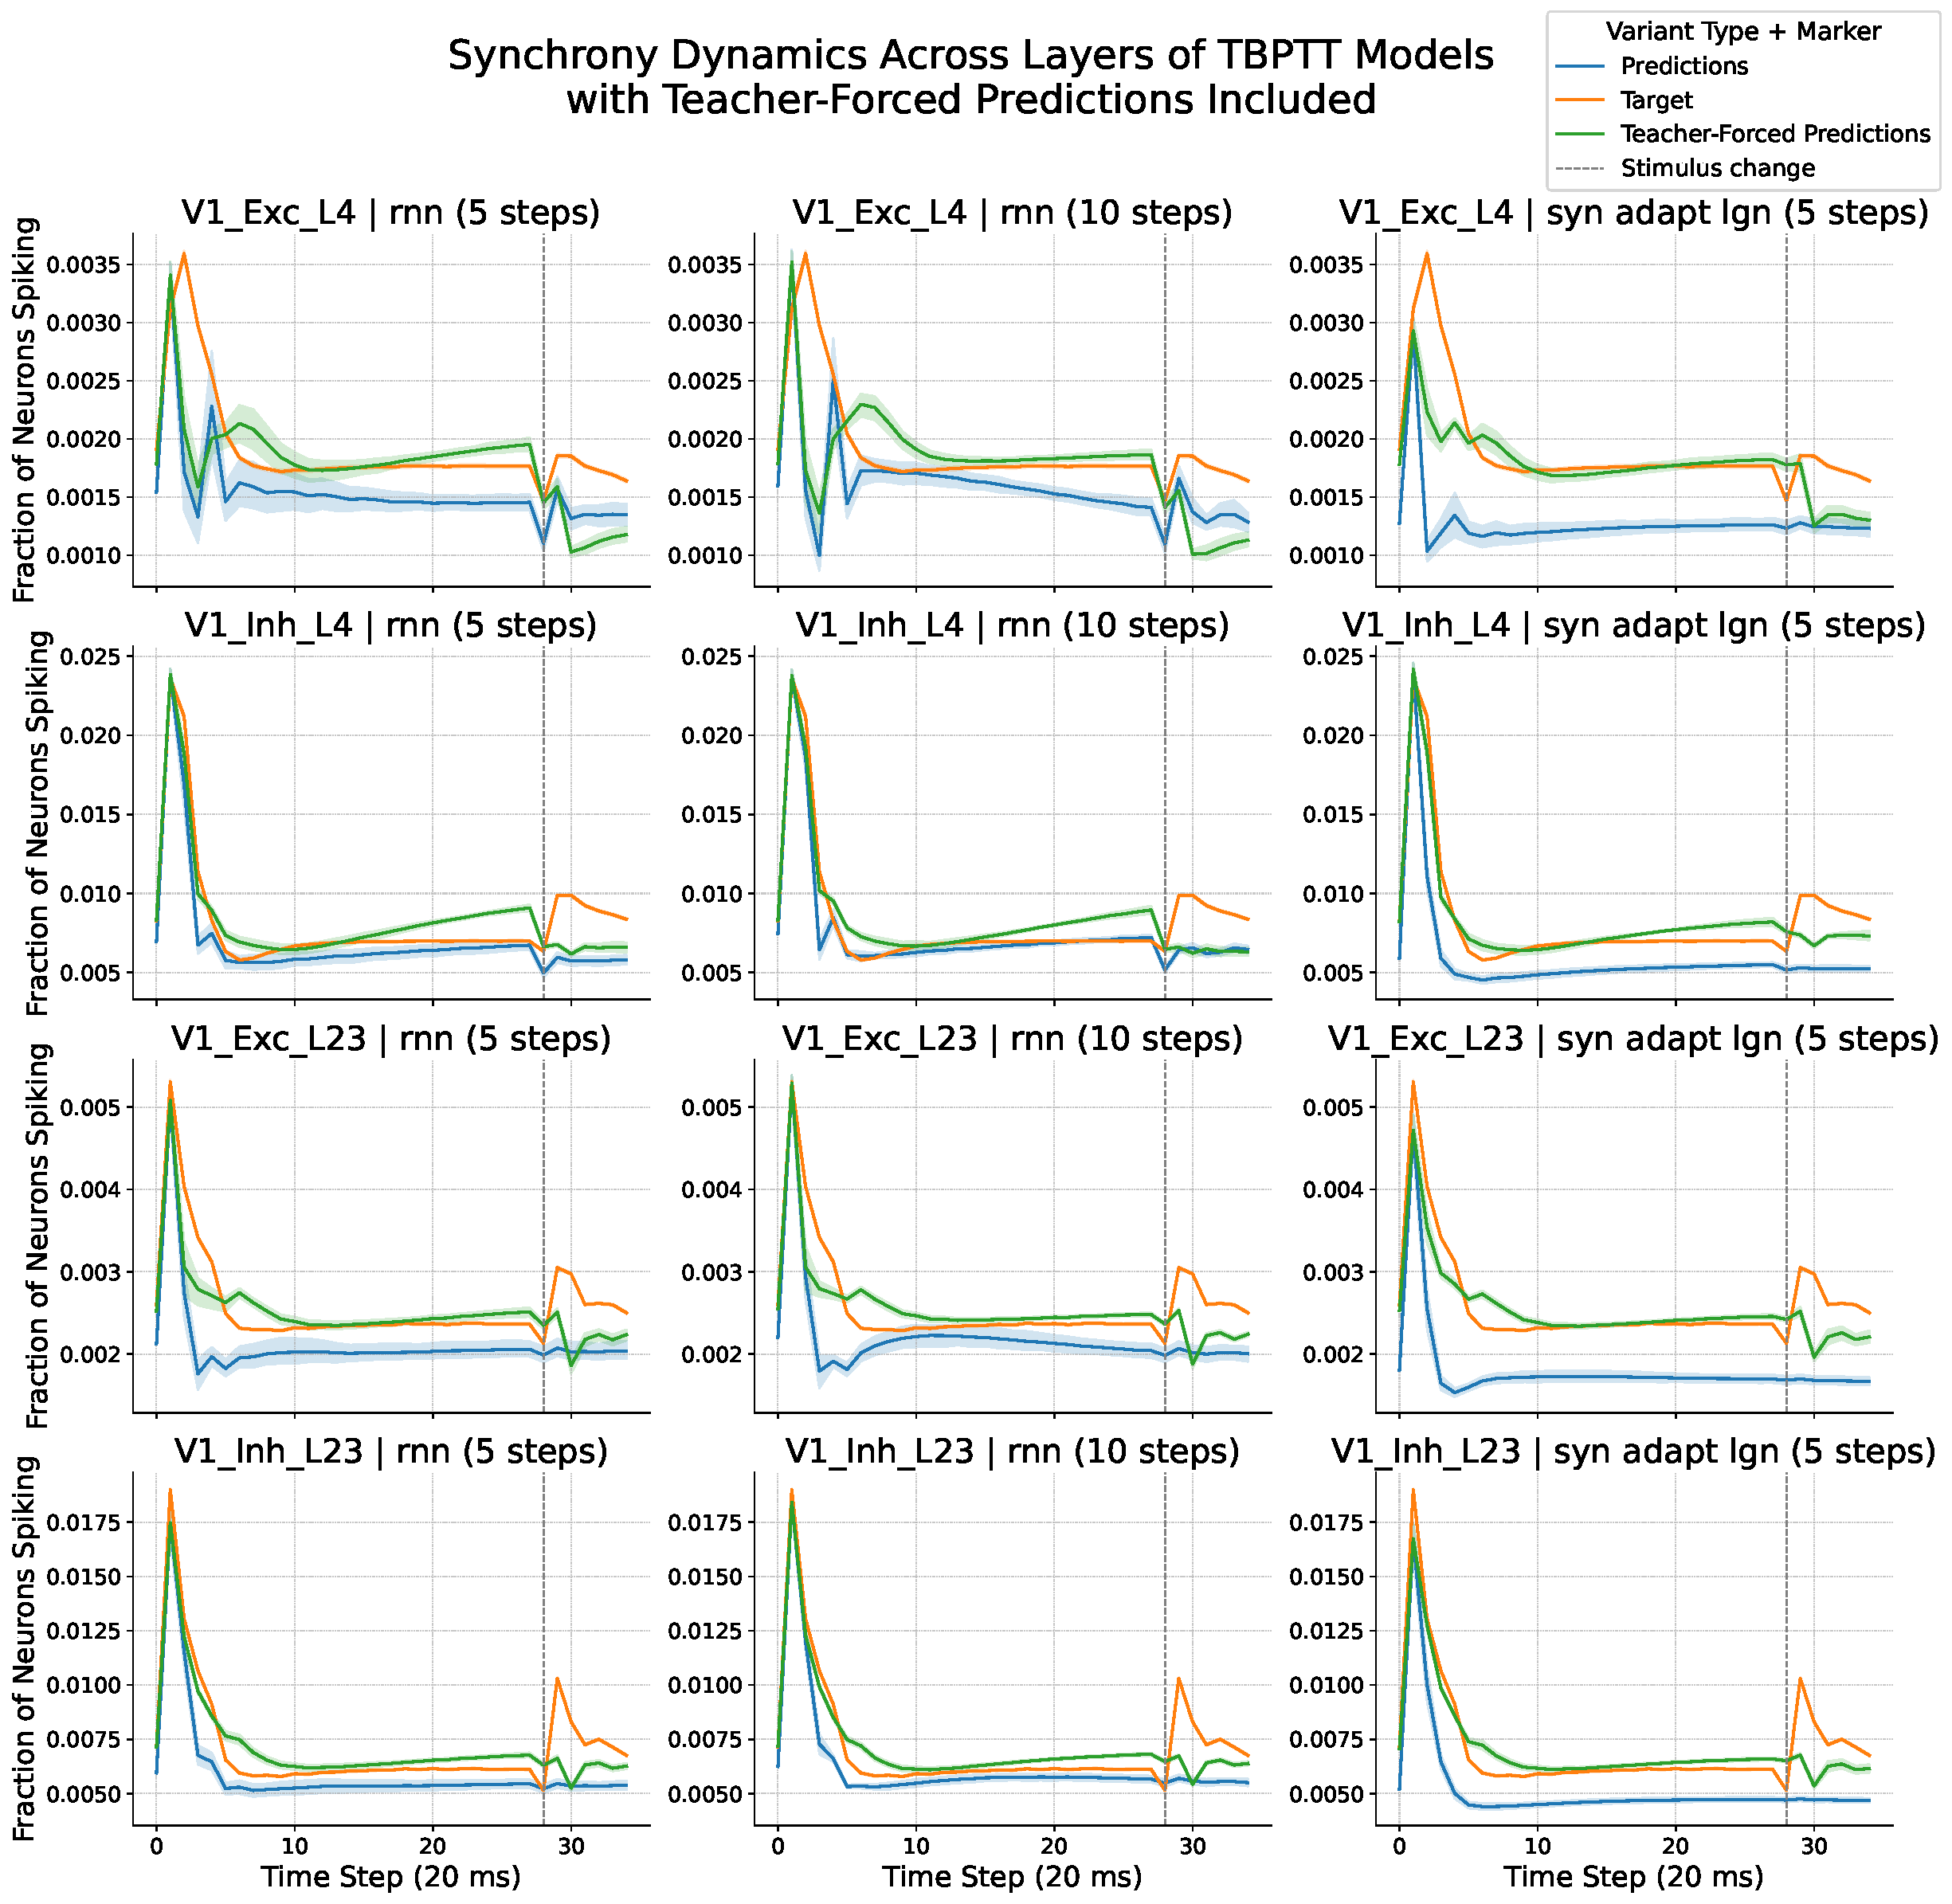
\includegraphics[width=\linewidth]{img/plots/tbptt_models_forced_included_model_synchrony_curve.pdf}
    \caption{This figure depicts mean synchrony curve of all model variants using TBPTT training algorithm. It depicts their predictions, teacher-forced predictions and its comparison to mean target synchrony curve both across all trials and all model subset variants including error bars. The dashed line marks the time step where the natural stimuli and blank stimuli changes.}
    \label{fig:free_vs_teacher_forced_synchrony}
\end{figure}

From the plot of the synchronies we can see that the prediction dynamics slightly improve in the initial natural stimuli stages and in the change of the stimuli from natural to blank. Interestingly thought, it seems that it is neither successful in capturing of the higher spontaneous neuronal responses in the blank stages. However, we see increase dynamic in these stages that might be a promising sign. Interestingly, the teacher-forced predictions seems to deviate in the later natural stimuli activity from the target sequence in the layer IV responses of the rnn model variants. 

Finally, there is an interesting behavior of the teacher-forced stimuli in the synaptic depression model that seems to have the best overall temporal behavior of the predictions across all the models that is also confirmed by the boxplot of the synchrony CC in the Figure~\ref{fig:boxplot_models_pearson_synchrony_different_layers}. This might be sign of not ideal training procedure in the synaptic depression model and that the model failed to properly predict the following stages of the sequence. It is also the sign though that while the predictions improve the model might outperform all of the tested models. The fact that we would expect since we enhance the biological plausibility of the model.

\subsubsection{Drift Between Synchrony Curves of Teacher-Forced and Free Predictions}
\label{subsubsec:drift_teacher_free_synchrony}

In the last part of this section we focus on the difference between the teacher-forced and free prediction synchrony curves also called as \emph{drift}. This is depicted for each layer separately in the Figure~\ref{fig:teacher_forced_free_drift}. This metric can unveil influence of the state reset in the different time steps and potentially show the distraction of our model throught time.

\begin{figure}
    \centering
    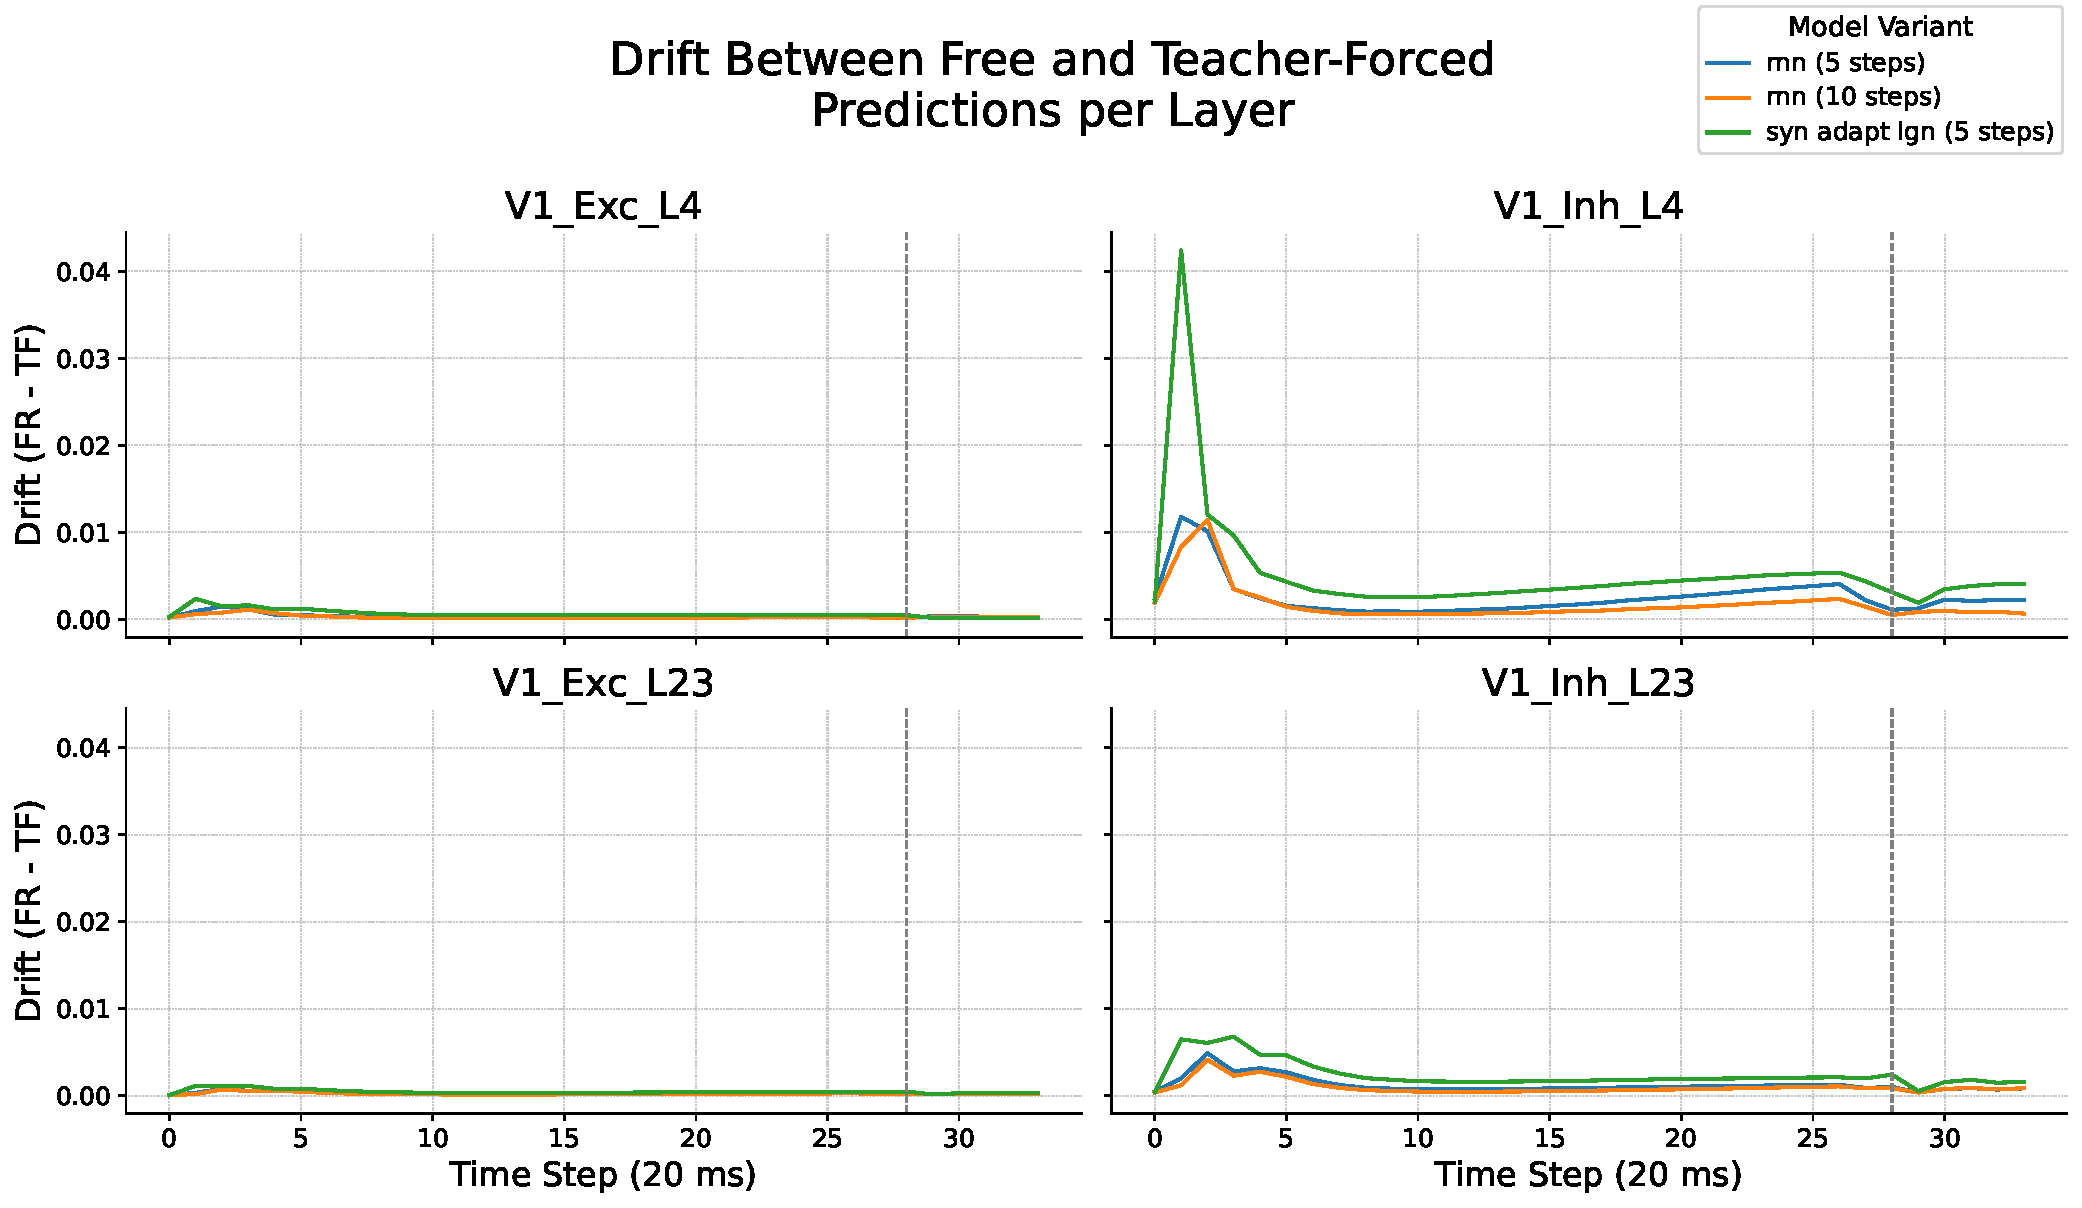
\includegraphics[width=\linewidth]{img/plots/temporal_drift_forced_free.pdf}
    \caption{This figure depicts plot of temporal dependency of the difference between teacher-forced and normal prediction (free) synchrony curves across the experiment duration per all experiments each layer separately. We call this metric as "drift". In the figure we compare models using TBPTT training algorithm.}
    \label{fig:teacher_forced_free_drift}
\end{figure}

As we can see the highest drift is across all tested model variants during the initial natural stimulus stage, the most active stage in terms of neuronal activity. As we can see there is a clearly highest drift throughout the time in the synaptic depression model. That supports our hypothesis about the non-ideal training of this model variant. The positive aspect that we can read from these results is that the model predictions does not really worsen in the later stages of the sequence indicating that the model can predict the temporal sequence pretty well. Its predictions mainly differ in the highly dynamical neuronal stages of the experiment that we might also consider as the most challenging one.

Overall, it seems to us that mainly the synaptic depression model seems to have higher potential in prediction of the temporal activity while looking at the teacher-forced predictions and that it might be worth it focus on the fideling out of the training procedure of this model type.

\subsection{Hyperparameter Grid Search}

\begin{table}
    \centering\footnotesize\sf
    \begin{tabular}{ccc}
    \toprule
    lr & N-CC & P-CC \\
    \midrule
    0.000008 & 0.350904 & 0.285114 \\
    0.000005 & 0.350027 & 0.284416 \\
    0.000010 & 0.270970 & 0.220144 \\
    0.000025 & 0.187077 & 0.151972 \\
    0.000050 & 0.114566 & 0.093056 \\
    0.000500 & 0.097858 & 0.079533 \\
    0.000075 & 0.077174 & 0.062676 \\
    0.000100 & 0.037527 & 0.030460 \\
    \bottomrule
    \end{tabular}
    \caption{\textbf{Grid Search Summary for simple (tanh) Model.} This table depicts grid search results summary conducted on the simple (tanh) model. It has been done using only one model subset variant across all grid search in this thesis. The labels of each table symbolize: "lr" - learning rate, "N-CC" - normalized cross correlation, "P-CC" - pearson correlation coefficient.}
    \label{tab:grid_simple_tanh}
\end{table}

\begin{table}
    \centering\footnotesize\sf
    \begin{tabular}{ccc}
    \toprule
    lr & N-CC & P-CC \\
    \midrule
    0.000100 & 0.878693 & 0.714005 \\
    0.000075 & 0.877059 & 0.712670 \\
    0.000050 & 0.872625 & 0.709055 \\
    0.000500 & 0.794590 & 0.645656 \\
    0.000025 & 0.294032 & 0.238913 \\
    0.000010 & 0.010441 & 0.008462 \\
    0.000005 & 0.001354 & 0.001069 \\
    0.000008 & 0.000050 & 0.000018 \\
    \bottomrule
    \end{tabular}
    \caption{\textbf{Grid Search Summary for simple (leakytanh) Model.} This table depicts grid search results summary conducted on the simple (leakytanh) model. It has been done using only one model subset variant across all grid search in this thesis. The labels of each table symbolize: "lr" - learning rate, "N-CC" - normalized cross correlation, "P-CC" - pearson correlation coefficient.}
    \label{tab:grid_simple_leakytanh}
\end{table}

\begin{table}
    \centering\footnotesize\sf
    \begin{tabular}{cccccc}
    \toprule
    lr & n-ls & n-nl & n-res & N-CC & P-CC \\
    \midrule
    0.000010 & 10 & 3 & True & 0.880114 & 0.715163 \\
    0.000010 & 10 & 7 & True & 0.879289 & 0.714492 \\
    0.000008 & 10 & 3 & True & 0.878549 & 0.713885 \\
    0.000008 & 10 & 7 & True & 0.878224 & 0.713618 \\
    0.000008 & 10 & 5 & True & 0.877150 & 0.712746 \\
    0.000010 & 5 & 5 & True & 0.876449 & 0.712174 \\
    0.000010 & 5 & 7 & True & 0.871925 & 0.708491 \\
    0.000010 & 10 & 5 & True & 0.871830 & 0.708410 \\
    0.000008 & 5 & 5 & True & 0.866316 & 0.703933 \\
    0.000010 & 5 & 3 & True & 0.860474 & 0.699177 \\
    0.000008 & 5 & 7 & True & 0.857937 & 0.697110 \\
    0.000010 & 5 & 5 & False & 0.854195 & 0.694092 \\
    0.000010 & 10 & 3 & False & 0.825813 & 0.670711 \\
    0.000008 & 10 & 3 & False & 0.813353 & 0.660599 \\
    0.000010 & 10 & 5 & False & 0.798817 & 0.648800 \\
    0.000010 & 5 & 3 & False & 0.766755 & 0.623028 \\
    0.000008 & 5 & 7 & False & 0.759580 & 0.617220 \\
    0.000008 & 10 & 7 & False & 0.751363 & 0.610289 \\
    0.000008 & 5 & 5 & False & 0.723905 & 0.587979 \\
    0.000010 & 10 & 7 & False & 0.722965 & 0.587225 \\
    0.000008 & 10 & 5 & False & 0.626814 & 0.509143 \\
    0.000008 & 5 & 3 & True & 0.295512 & 0.240123 \\
    0.000008 & 5 & 3 & False & 0.008394 & 0.006809 \\
    0.000010 & 5 & 7 & False & -0.259292 & -0.210666 \\
    \bottomrule
    \end{tabular}
    \caption{\textbf{Grid Search Summary for dnn joint Model.} This table depicts grid search results summary conducted on the dnn joint model. It has been done using only one model subset variant across all grid search in this thesis. The labels of each table symbolize: "lr" - learning rate, "n-ls" - layer size of the module of neuron, "n-nl" - number of layers of the neuron module, "n-res" - flag whether the neuron module use residual connection, "N-CC" - normalized cross correlation, "P-CC" - pearson correlation coefficient.}
    \label{tab:grid_dnn_joint}
\end{table}


\begin{table}
    \centering\footnotesize\sf
    \begin{tabular}{cccc}
    \toprule
    lr & n-tbptt & N-CC & P-CC \\
    \midrule
    0.000030 & 10 & 0.933978 & 0.758967 \\
    0.000030 & 5 & 0.932902 & 0.758091 \\
    0.000050 & 10 & 0.932787 & 0.757994 \\
    0.000010 & 5 & 0.914351 & 0.743027 \\
    0.000030 & 20 & 0.913769 & 0.742504 \\
    0.000010 & 10 & 0.911943 & 0.741078 \\
    0.000050 & 40 & 0.911054 & 0.740291 \\
    0.000050 & 5 & 0.885195 & 0.719318 \\
    0.000010 & 20 & 0.873075 & 0.709455 \\
    0.000050 & 20 & 0.829914 & 0.674317 \\
    0.000030 & 40 & 0.689550 & 0.560315 \\
    0.000010 & 40 & 0.281750 & 0.228879 \\
    \bottomrule
    \end{tabular}
    \caption{\textbf{Grid Search Summary for rnn separate Model.} This table depicts grid search results summary conducted on the rnn separate model. It has been done using only one model subset variant across all grid search in this thesis. The labels of each table symbolize: "lr" - learning rate, "n-tbptt" - number of TBPTT time steps, "N-CC" - normalized cross correlation, "P-CC" - pearson correlation coefficient.}
    \label{tab:grid_rnn_separate}
\end{table}

\begin{table}
    \centering\footnotesize\sf
    \begin{tabular}{cccc}
    \toprule
    lr & n-tbptt & N-CC & P-CC \\
    \midrule
    0.000030 & 5 & 0.904516 & 0.734752 \\
    0.000050 & 10 & 0.858861 & 0.697665 \\
    0.000010 & 5 & 0.826371 & 0.671237 \\
    0.000010 & 10 & 0.728944 & 0.592099 \\
    0.000050 & 5 & 0.678222 & 0.550937 \\
    0.000030 & 10 & -0.016808 & -0.013631 \\
    \bottomrule
    \end{tabular}
    \caption{\textbf{Grid Search Summary for synaptic adaptation Model.} This table depicts grid search results summary conducted on the synaptic adaptation model. It has been done using only one model subset variant across all grid search in this thesis. The labels of each table symbolize: "lr" - learning rate, "n-tbptt" - number of TBPTT time steps, "N-CC" - normalized cross correlation, "P-CC" - pearson correlation coefficient.}
    \label{tab:grid_synaptic_adaptation}
\end{table}


\subsection{Dependency of Train Dataset Size on Model Performance}

\begin{figure}
    \centering
    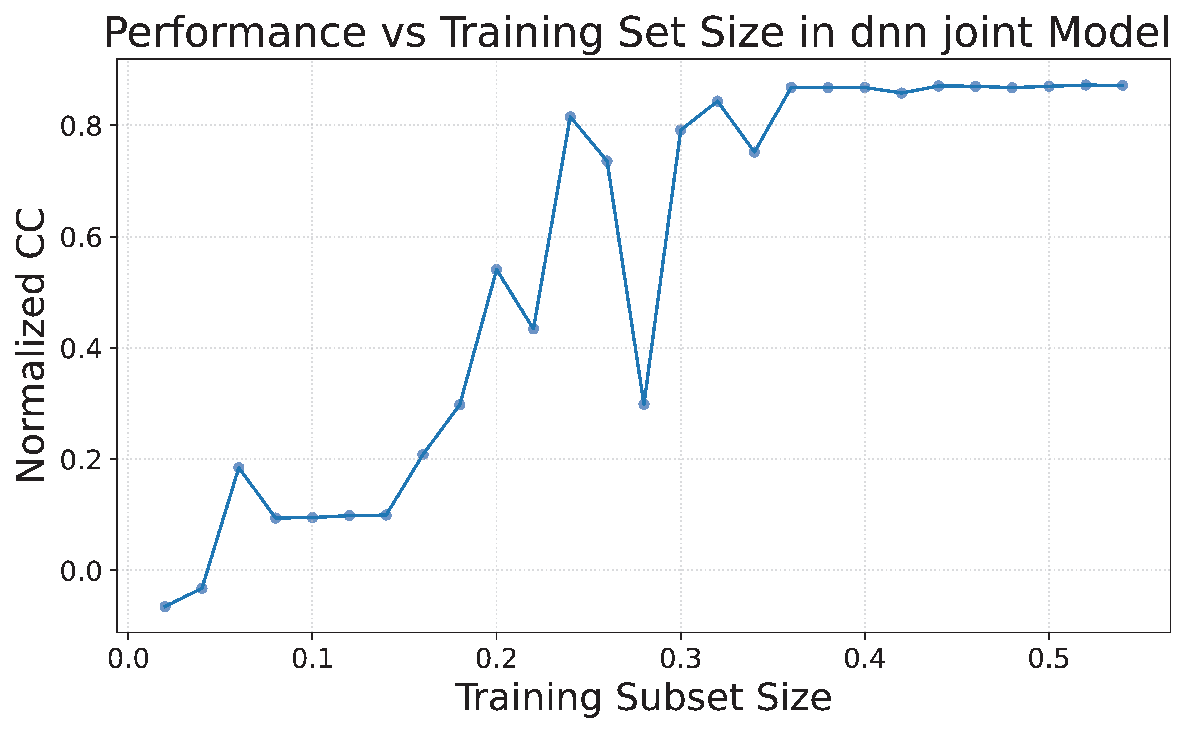
\includegraphics[width=0.8\linewidth]{img/plots/train_size_performance_dependency.pdf}
    \caption{This figure depicts dependency of normalized CC on training set size while training dnn joint model with hyperparameters used in model evaluation (Table~\ref{tab:evaluation_setup}). The figure depicts the variants of subset sizes only until subset size 0.54 of the original training dataset due the not enough computational resources for comprehensive analysis on all subset size variants. However, it seems that the performance already stabilized and we do not expect massive changes in behavior for the larger subsets of original training dataset.}
    \label{fig:train_size_cc_norm_dependency}
\end{figure}

\chapwithtoc{Conclusion}

This thesis focused on developing a recurrent neural network (RNN) that mimics the spiking activity of a spiking neural network (SNN) modeling the cat's primary visual cortex (V1), as proposed by \citet{antolik2024comprehensive}, while incorporating known biological constraints of the system. The overarching goal was to construct an explainable model of V1 using deep neural network techniques. Throughout the thesis, we arrived at several key findings.

We first implemented a base RNN model whose architecture directly maps each neuron in the SNN to a corresponding neuron in the RNN, reflecting a simplified version of the biological V1's layered structure. Due to computational constraints, we limited the model to randomly selected subsets of neurons from each population and reduced the temporal resolution from 1~ms to 20~ms. We further introduced several biologically inspired modules to improve both model interpretability and performance. These included shared neural network modules per neuron, acting as trainable, complex replacements for standard activation functions, and synaptic depression modules that modify neuronal inputs in a manner analogous to biological synaptic depression.

Our results demonstrate that the addition of biologically motivated modules improves model performance both in terms of general predictive metrics (such as normalized cross-correlation) and in capturing the temporal dynamics of neuronal responses, as reflected by temporal behavior curves across neuronal populations. The best-performing model variants showed promising fidelity in reproducing the temporal behavior of the SNN, supporting the notion that integrating anatomical constraints into deep neural network architectures holds significant promise for modeling neural activity.

This hybrid modeling approach, which draws from the strengths of both deep learning and biologically grounded methods, may provide a scalable and interpretable framework for neural system modeling. Deep neural networks offer strong performance across various tasks and benefit from continuous improvements in scalability and training efficiency. By embedding biological constraints into their structure, we gain insights into neural function and mitigate the common criticism of DNNs as "black box" models.

Importantly, this research contributes to the growing field of biologically inspired artificial intelligence. It demonstrates a practical method for combining the computational power of deep learning with the structural interpretability of biological modeling, laying the groundwork for future interdisciplinary applications in computational neuroscience, machine learning, and brain-computer interface development.

However, several limitations emerged. Most notably, the models struggled to accurately predict spontaneous neuronal activity during blank stimulus phases, pointing to incomplete modeling of temporal behavior. In particular, the most biologically complex variant, the model incorporating synaptic depression, performed worse than expected. We attribute this to limited computational resources and the high complexity of the model. Furthermore, although this study benefited from full knowledge of the target model (the SNN), real-world scenarios often lack such ground truth data. Despite this advantage, reproducing the SNN's responses remains a challenging task, underscoring the inherent complexity of modeling the primary visual cortex.

\subsection*{Future Work}
In the end, we would like to outline the possible future research directions. 

First, there is substantial room for improvement in hyperparameter tuning, particularly for the synaptic depression model. More fine-grained hyperparameter selection, extended training durations, and access to enhanced computational resources may resolve the shortcomings observed in our current implementation.

Once these optimizations are in place, the model should be tested on real biological datasets. This would involve withholding some neuronal responses during training and evaluating the model's ability to predict these unseen targets—closely mimicking conditions typical in neuroscience, where only limited neuronal recordings are available.

Upon successful performance under these conditions, the model should be fine-tuned using biological recordings, especially from macaque V1 tracking experiments, which were initially intended to be part of this thesis. Due to the complexity of the task, this component was deferred. However, strong performance on real biological data could mark a significant advancement in our capacity to model neural systems and improve our understanding of the visual cortex.

Ultimately, we envision integrating this framework with the comprehensive SNN model of V1 by \citet{antolik2024comprehensive}, thus enabling deeper and more interpretable analyses of the visual system.

Conclusively, this work represents a foundational step toward merging computational power with biological fidelity, bringing us closer to truly interpretable models of brain function.


\ifEN
\chapwithtoc{Bibliography}
\else
\chapwithtoc{Seznam použité literatury}
\fi

\printbibliography[heading=none]


\appendix
\chapter{Model Implementation and Evaluation Tools}
A significant portion of the work for this thesis was dedicated to preprocessing the dataset from the source SNN model, developing the RNN model, and creating an evaluation framework. All source code related to these functionalities is included in the thesis attachment, accompanied by documentation providing comprehensive descriptions of each tool.

Throughout the project, development was managed using a GitHub version control repository, where the most up-to-date version of the thesis source code remains available. The attachment provided with this thesis is a snapshot of our working branch \verb|model_restruct|. Due to file type restrictions and large file size, a small example dataset was removed from the attachment. For access to an example dataset, the latest project version, or to review the development history, please refer to the project's GitHub repository:\footnote{\url{https://github.com/dbeinhauer/mcs-source}}.

It should be noted that a small portion of the codebase was contributed by another student, Richard Kraus, who worked on enhancing the model architecture by applying spatial constraints. This contribution is primarily encapsulated in the source file \verb|nn_model/connection_learning.py|. However, this functionality was not incorporated into the implementation discussed throughout this thesis and remains an optional plugin for potential future model extensions. Additionally, Richard Kraus made several minor contributions to other parts of the codebase, aimed at improving memory and computational efficiency, as well as aiding in the installation process on the MetaCentrum\footnote{\url{https://metavo.metacentrum.cz/}} computational cluster. All contributions can be tracked in the GitHub repository.

The dataset utilized throughout this thesis and the evaluation results are stored on the Wintermute cluster of the CSNG MFF CUNI group, with storage details further specified in the attached documentation.



% if your attachments are complicated, describe them in a separate appendix
%\include{attachments}

\openright
\end{document}
